\documentclass[12pt,a4paper]{article}

% FONTS
\usepackage{microtype}
\usepackage{graphicx}  % to include figures (can also use other packages)
\usepackage{color}

% LAYOUT
\textheight=230mm
\textwidth=160mm
\oddsidemargin=7mm
\evensidemargin=-10mm
\topmargin=-10mm
\headsep=20mm
\columnsep=5mm
\addtolength{\belowcaptionskip}{0.5em}

\renewcommand{\textfraction}{0.01}
\renewcommand{\floatpagefraction}{0.99}
\renewcommand{\topfraction}{0.9}
\renewcommand{\bottomfraction}{0.9}


\setlength{\hoffset}{-2cm}
\setlength{\voffset}{-2cm}
% Page defaults ...
\topmargin=0.5cm
\oddsidemargin=2.5cm
\textwidth=16cm
\textheight=22cm
% Allow the page size to vary a bit ...
\raggedbottom
% To avoid Latex to be too fussy with line breaking ...
\sloppy

% MATH
\usepackage{amsmath} % Adds a large collection of math symbols
\usepackage{amssymb}
\usepackage{amsfonts}
\usepackage{upgreek} % Adds in support for greek letters in roman typeset

\usepackage{siunitx}
% Unit typesetting
\sisetup{
  detect-weight = true, 
  separate-uncertainty=true,
  uncertainty-separator = {\,},
  list-units = single
}

\usepackage{ifthen} % for conditional statements
\usepackage{xspace} % To avoid problems with missing or double spaces after predefined symbols
\newboolean{uprightparticles}
\setboolean{uprightparticles}{false} %True for upright particle symbols
%%% $Id: lhcb-symbols-def.tex 90362 2016-04-07 13:38:32Z pkoppenb $
%%% ======================================================================
%%% Purpose: Standard LHCb aliases
%%% Author: Originally Ulrik Egede, adapted by Tomasz Skwarnicki for templates,
%%% rewritten by Chris Parkes
%%% Maintainer : Ulrik Egede (2010 - 2012)
%%% Maintainer : Rolf Oldeman (2012 - 2014)
%%% =======================================================================

%%% To use this file outside the normal LHCb document environment, the
%%% following should be added in a preamble (before \begin{document}
%%%
%%%\usepackage{ifthen} 
%%%\newboolean{uprightparticles}
%%%\setboolean{uprightparticles}{false} %Set true for upright particle symbols
\usepackage{xspace} 
\usepackage{upgreek}

%%%%%%%%%%%%%%%%%%%%%%%%%%%%%%%%%%%%%%%%%%%%%%%%%%%%%%%%%%%%
%%%
%%% The following is to ensure that the template automatically can process
%%% this file.
%%%
%%% Add comments with at least three %%% preceding.
%%% Add new sections with one % preceding
%%% Add new subsections with two %% preceding
%%%%%%%%%%%%%%%%%%%%%%%%%%%%%%%%%%%%%%%%%%%%%%%%%%%%%%%%%%%%

%%%%%%%%%%%%%
% Experiments
%%%%%%%%%%%%%
\def\lhcb {\mbox{LHCb}\xspace}
\def\atlas  {\mbox{ATLAS}\xspace}
\def\cms    {\mbox{CMS}\xspace}
\def\alice  {\mbox{ALICE}\xspace}
\def\babar  {\mbox{BaBar}\xspace}
\def\belle  {\mbox{Belle}\xspace}
\def\cleo   {\mbox{CLEO}\xspace}
\def\cdf    {\mbox{CDF}\xspace}
\def\dzero  {\mbox{D0}\xspace}
\def\aleph  {\mbox{ALEPH}\xspace}
\def\delphi {\mbox{DELPHI}\xspace}
\def\opal   {\mbox{OPAL}\xspace}
\def\lthree {\mbox{L3}\xspace}
\def\sld    {\mbox{SLD}\xspace}
%%%\def\argus  {\mbox{ARGUS}\xspace}
%%%\def\uaone  {\mbox{UA1}\xspace}
%%%\def\uatwo  {\mbox{UA2}\xspace}
%%%\def\ux85 {\mbox{UX85}\xspace}
\def\cern {\mbox{CERN}\xspace}
\def\lhc    {\mbox{LHC}\xspace}
\def\lep    {\mbox{LEP}\xspace}
\def\tevatron {Tevatron\xspace}

%% LHCb sub-detectors and sub-systems

%%%\def\pu     {PU\xspace}
\def\velo   {VELO\xspace}
\def\rich   {RICH\xspace}
\def\richone {RICH1\xspace}
\def\richtwo {RICH2\xspace}
\def\ttracker {TT\xspace}
\def\intr   {IT\xspace}
\def\st     {ST\xspace}
\def\ot     {OT\xspace}
%%%\def\Tone   {T1\xspace}
%%%\def\Ttwo   {T2\xspace}
%%%\def\Tthree {T3\xspace}
%%%\def\Mone   {M1\xspace}
%%%\def\Mtwo   {M2\xspace}
%%%\def\Mthree {M3\xspace}
%%%\def\Mfour  {M4\xspace}
%%%\def\Mfive  {M5\xspace}
\def\spd    {SPD\xspace}
\def\presh  {PS\xspace}
\def\ecal   {ECAL\xspace}
\def\hcal   {HCAL\xspace}
%%%\def\bcm    {BCM\xspace}
\def\MagUp {\mbox{\em Mag\kern -0.05em Up}\xspace}
\def\MagDown {\mbox{\em MagDown}\xspace}

\def\ode    {ODE\xspace}
\def\daq    {DAQ\xspace}
\def\tfc    {TFC\xspace}
\def\ecs    {ECS\xspace}
\def\lone   {L0\xspace}
\def\hlt    {HLT\xspace}
\def\hltone {HLT1\xspace}
\def\hlttwo {HLT2\xspace}

%%% Upright (not slanted) Particles

\ifthenelse{\boolean{uprightparticles}}%
{\def\Palpha      {\ensuremath{\upalpha}\xspace}
 \def\Pbeta       {\ensuremath{\upbeta}\xspace}
 \def\Pgamma      {\ensuremath{\upgamma}\xspace}                 
 \def\Pdelta      {\ensuremath{\updelta}\xspace}                 
 \def\Pepsilon    {\ensuremath{\upepsilon}\xspace}                 
 \def\Pvarepsilon {\ensuremath{\upvarepsilon}\xspace}                 
 \def\Pzeta       {\ensuremath{\upzeta}\xspace}                 
 \def\Peta        {\ensuremath{\upeta}\xspace}                 
 \def\Ptheta      {\ensuremath{\uptheta}\xspace}                 
 \def\Pvartheta   {\ensuremath{\upvartheta}\xspace}                 
 \def\Piota       {\ensuremath{\upiota}\xspace}                 
 \def\Pkappa      {\ensuremath{\upkappa}\xspace}                 
 \def\Plambda     {\ensuremath{\uplambda}\xspace}                 
 \def\Pmu         {\ensuremath{\upmu}\xspace}                 
 \def\Pnu         {\ensuremath{\upnu}\xspace}                 
 \def\Pxi         {\ensuremath{\upxi}\xspace}                 
 \def\Ppi         {\ensuremath{\uppi}\xspace}                 
 \def\Pvarpi      {\ensuremath{\upvarpi}\xspace}                 
 \def\Prho        {\ensuremath{\uprho}\xspace}                 
 \def\Pvarrho     {\ensuremath{\upvarrho}\xspace}                 
 \def\Ptau        {\ensuremath{\uptau}\xspace}                 
 \def\Pupsilon    {\ensuremath{\upupsilon}\xspace}                 
 \def\Pphi        {\ensuremath{\upphi}\xspace}                 
 \def\Pvarphi     {\ensuremath{\upvarphi}\xspace}                 
 \def\Pchi        {\ensuremath{\upchi}\xspace}                 
 \def\Ppsi        {\ensuremath{\uppsi}\xspace}                 
 \def\Pomega      {\ensuremath{\upomega}\xspace}                 

 \def\PDelta      {\ensuremath{\Delta}\xspace}                 
 \def\PXi      {\ensuremath{\Xi}\xspace}                 
 \def\PLambda      {\ensuremath{\Lambda}\xspace}                 
 \def\PSigma      {\ensuremath{\Sigma}\xspace}                 
 \def\POmega      {\ensuremath{\Omega}\xspace}                 
 \def\PUpsilon      {\ensuremath{\Upsilon}\xspace}                 
 
 %\mathchardef\Deltares="7101
 %\mathchardef\Xi="7104
 %\mathchardef\Lambda="7103
 %\mathchardef\Sigma="7106
 %\mathchardef\Omega="710A


 \def\PA      {\ensuremath{\mathrm{A}}\xspace}                 
 \def\PB      {\ensuremath{\mathrm{B}}\xspace}                 
 \def\PC      {\ensuremath{\mathrm{C}}\xspace}                 
 \def\PD      {\ensuremath{\mathrm{D}}\xspace}                 
 \def\PE      {\ensuremath{\mathrm{E}}\xspace}                 
 \def\PF      {\ensuremath{\mathrm{F}}\xspace}                 
 \def\PG      {\ensuremath{\mathrm{G}}\xspace}                 
 \def\PH      {\ensuremath{\mathrm{H}}\xspace}                 
 \def\PI      {\ensuremath{\mathrm{I}}\xspace}                 
 \def\PJ      {\ensuremath{\mathrm{J}}\xspace}                 
 \def\PK      {\ensuremath{\mathrm{K}}\xspace}                 
 \def\PL      {\ensuremath{\mathrm{L}}\xspace}                 
 \def\PM      {\ensuremath{\mathrm{M}}\xspace}                 
 \def\PN      {\ensuremath{\mathrm{N}}\xspace}                 
 \def\PO      {\ensuremath{\mathrm{O}}\xspace}                 
 \def\PP      {\ensuremath{\mathrm{P}}\xspace}                 
 \def\PQ      {\ensuremath{\mathrm{Q}}\xspace}                 
 \def\PR      {\ensuremath{\mathrm{R}}\xspace}                 
 \def\PS      {\ensuremath{\mathrm{S}}\xspace}                 
 \def\PT      {\ensuremath{\mathrm{T}}\xspace}                 
 \def\PU      {\ensuremath{\mathrm{U}}\xspace}                 
 \def\PV      {\ensuremath{\mathrm{V}}\xspace}                 
 \def\PW      {\ensuremath{\mathrm{W}}\xspace}                 
 \def\PX      {\ensuremath{\mathrm{X}}\xspace}                 
 \def\PY      {\ensuremath{\mathrm{Y}}\xspace}                 
 \def\PZ      {\ensuremath{\mathrm{Z}}\xspace}                 
 \def\Pa      {\ensuremath{\mathrm{a}}\xspace}                 
 \def\Pb      {\ensuremath{\mathrm{b}}\xspace}                 
 \def\Pc      {\ensuremath{\mathrm{c}}\xspace}                 
 \def\Pd      {\ensuremath{\mathrm{d}}\xspace}                 
 \def\Pe      {\ensuremath{\mathrm{e}}\xspace}                 
 \def\Pf      {\ensuremath{\mathrm{f}}\xspace}                 
 \def\Pg      {\ensuremath{\mathrm{g}}\xspace}                 
 \def\Ph      {\ensuremath{\mathrm{h}}\xspace}                 
 \def\Pi      {\ensuremath{\mathrm{i}}\xspace}                 
 \def\Pj      {\ensuremath{\mathrm{j}}\xspace}                 
 \def\Pk      {\ensuremath{\mathrm{k}}\xspace}                 
 \def\Pl      {\ensuremath{\mathrm{l}}\xspace}                 
 \def\Pm      {\ensuremath{\mathrm{m}}\xspace}                 
 \def\Pn      {\ensuremath{\mathrm{n}}\xspace}                 
 \def\Po      {\ensuremath{\mathrm{o}}\xspace}                 
 \def\Pp      {\ensuremath{\mathrm{p}}\xspace}                 
 \def\Pq      {\ensuremath{\mathrm{q}}\xspace}                 
 \def\Pr      {\ensuremath{\mathrm{r}}\xspace}                 
 \def\Ps      {\ensuremath{\mathrm{s}}\xspace}                 
 \def\Pt      {\ensuremath{\mathrm{t}}\xspace}                 
 \def\Pu      {\ensuremath{\mathrm{u}}\xspace}                 
 \def\Pv      {\ensuremath{\mathrm{v}}\xspace}                 
 \def\Pw      {\ensuremath{\mathrm{w}}\xspace}                 
 \def\Px      {\ensuremath{\mathrm{x}}\xspace}                 
 \def\Py      {\ensuremath{\mathrm{y}}\xspace}                 
 \def\Pz      {\ensuremath{\mathrm{z}}\xspace}                 
}
{\def\Palpha      {\ensuremath{\alpha}\xspace}
 \def\Pbeta       {\ensuremath{\beta}\xspace}
 \def\Pgamma      {\ensuremath{\gamma}\xspace}                 
 \def\Pdelta      {\ensuremath{\delta}\xspace}                 
 \def\Pepsilon    {\ensuremath{\epsilon}\xspace}                 
 \def\Pvarepsilon {\ensuremath{\varepsilon}\xspace}                 
 \def\Pzeta       {\ensuremath{\zeta}\xspace}                 
 \def\Peta        {\ensuremath{\eta}\xspace}                 
 \def\Ptheta      {\ensuremath{\theta}\xspace}                 
 \def\Pvartheta   {\ensuremath{\vartheta}\xspace}                 
 \def\Piota       {\ensuremath{\iota}\xspace}                 
 \def\Pkappa      {\ensuremath{\kappa}\xspace}                 
 \def\Plambda     {\ensuremath{\lambda}\xspace}                 
 \def\Pmu         {\ensuremath{\mu}\xspace}                 
 \def\Pnu         {\ensuremath{\nu}\xspace}                 
 \def\Pxi         {\ensuremath{\xi}\xspace}                 
 \def\Ppi         {\ensuremath{\pi}\xspace}                 
 \def\Pvarpi      {\ensuremath{\varpi}\xspace}                 
 \def\Prho        {\ensuremath{\rho}\xspace}                 
 \def\Pvarrho     {\ensuremath{\varrho}\xspace}                 
 \def\Ptau        {\ensuremath{\tau}\xspace}                 
 \def\Pupsilon    {\ensuremath{\upsilon}\xspace}                 
 \def\Pphi        {\ensuremath{\phi}\xspace}                 
 \def\Pvarphi     {\ensuremath{\varphi}\xspace}                 
 \def\Pchi        {\ensuremath{\chi}\xspace}                 
 \def\Ppsi        {\ensuremath{\psi}\xspace}                 
 \def\Pomega      {\ensuremath{\omega}\xspace}                 
 \mathchardef\PDelta="7101
 \mathchardef\PXi="7104
 \mathchardef\PLambda="7103
 \mathchardef\PSigma="7106
 \mathchardef\POmega="710A
 \mathchardef\PUpsilon="7107
 \def\PA      {\ensuremath{A}\xspace}                 
 \def\PB      {\ensuremath{B}\xspace}                 
 \def\PC      {\ensuremath{C}\xspace}                 
 \def\PD      {\ensuremath{D}\xspace}                 
 \def\PE      {\ensuremath{E}\xspace}                 
 \def\PF      {\ensuremath{F}\xspace}                 
 \def\PG      {\ensuremath{G}\xspace}                 
 \def\PH      {\ensuremath{H}\xspace}                 
 \def\PI      {\ensuremath{I}\xspace}                 
 \def\PJ      {\ensuremath{J}\xspace}                 
 \def\PK      {\ensuremath{K}\xspace}                 
 \def\PL      {\ensuremath{L}\xspace}                 
 \def\PM      {\ensuremath{M}\xspace}                 
 \def\PN      {\ensuremath{N}\xspace}                 
 \def\PO      {\ensuremath{O}\xspace}                 
 \def\PP      {\ensuremath{P}\xspace}                 
 \def\PQ      {\ensuremath{Q}\xspace}                 
 \def\PR      {\ensuremath{R}\xspace}                 
 \def\PS      {\ensuremath{S}\xspace}                 
 \def\PT      {\ensuremath{T}\xspace}                 
 \def\PU      {\ensuremath{U}\xspace}                 
 \def\PV      {\ensuremath{V}\xspace}                 
 \def\PW      {\ensuremath{W}\xspace}                 
 \def\PX      {\ensuremath{X}\xspace}                 
 \def\PY      {\ensuremath{Y}\xspace}                 
 \def\PZ      {\ensuremath{Z}\xspace}                 
 \def\Pa      {\ensuremath{a}\xspace}                 
 \def\Pb      {\ensuremath{b}\xspace}                 
 \def\Pc      {\ensuremath{c}\xspace}                 
 \def\Pd      {\ensuremath{d}\xspace}                 
 \def\Pe      {\ensuremath{e}\xspace}                 
 \def\Pf      {\ensuremath{f}\xspace}                 
 \def\Pg      {\ensuremath{g}\xspace}                 
 \def\Ph      {\ensuremath{h}\xspace}                 
 \def\Pi      {\ensuremath{i}\xspace}                 
 \def\Pj      {\ensuremath{j}\xspace}                 
 \def\Pk      {\ensuremath{k}\xspace}                 
 \def\Pl      {\ensuremath{l}\xspace}                 
 \def\Pm      {\ensuremath{m}\xspace}                 
 \def\Pn      {\ensuremath{n}\xspace}                 
 \def\Po      {\ensuremath{o}\xspace}                 
 \def\Pp      {\ensuremath{p}\xspace}                 
 \def\Pq      {\ensuremath{q}\xspace}                 
 \def\Pr      {\ensuremath{r}\xspace}                 
 \def\Ps      {\ensuremath{s}\xspace}                 
 \def\Pt      {\ensuremath{t}\xspace}                 
 \def\Pu      {\ensuremath{u}\xspace}                 
 \def\Pv      {\ensuremath{v}\xspace}                 
 \def\Pw      {\ensuremath{w}\xspace}                 
 \def\Px      {\ensuremath{x}\xspace}                 
 \def\Py      {\ensuremath{y}\xspace}                 
 \def\Pz      {\ensuremath{z}\xspace}                 
}

%%%%%%%%%%%%%%%%%%%%%%%%%%%%%%%%%%%%%%%%%%%%%%%
% Particles
\makeatletter
\ifcase \@ptsize \relax% 10pt
  \newcommand{\miniscule}{\@setfontsize\miniscule{4}{5}}% \tiny: 5/6
\or% 11pt
  \newcommand{\miniscule}{\@setfontsize\miniscule{5}{6}}% \tiny: 6/7
\or% 12pt
  \newcommand{\miniscule}{\@setfontsize\miniscule{5}{6}}% \tiny: 6/7
\fi
\makeatother


\DeclareRobustCommand{\optbar}[1]{\shortstack{{\miniscule (\rule[.5ex]{1.25em}{.18mm})}
  \\ [-.7ex] $#1$}}


%% Leptons

\let\emi\en
\def\electron   {{\ensuremath{\Pe}}\xspace}
\def\en         {{\ensuremath{\Pe^-}}\xspace}   % electron negative (\em is taken)
\def\ep         {{\ensuremath{\Pe^+}}\xspace}
\def\epm        {{\ensuremath{\Pe^\pm}}\xspace} 
\def\epem       {{\ensuremath{\Pe^+\Pe^-}}\xspace}
%%%\def\ee         {\ensuremath{\Pe^-\Pe^-}\xspace}

\def\muon       {{\ensuremath{\Pmu}}\xspace}
\def\mup        {{\ensuremath{\Pmu^+}}\xspace}
\def\mun        {{\ensuremath{\Pmu^-}}\xspace} % muon negative (\mum is taken)
\def\mumu       {{\ensuremath{\Pmu^+\Pmu^-}}\xspace}

\def\tauon      {{\ensuremath{\Ptau}}\xspace}
\def\taup       {{\ensuremath{\Ptau^+}}\xspace}
\def\taum       {{\ensuremath{\Ptau^-}}\xspace}
\def\tautau     {{\ensuremath{\Ptau^+\Ptau^-}}\xspace}

\def\lepton     {{\ensuremath{\ell}}\xspace}
\def\ellm       {{\ensuremath{\ell^-}}\xspace}
\def\ellp       {{\ensuremath{\ell^+}}\xspace}
\def\ellell     {\ensuremath{\ell^+ \ell^-}\xspace}

\def\neu        {{\ensuremath{\Pnu}}\xspace}
\def\neub       {{\ensuremath{\overline{\Pnu}}}\xspace}
%%%\def\nuenueb    {\ensuremath{\neu\neub}\xspace}
\def\neue       {{\ensuremath{\neu_e}}\xspace}
\def\neueb      {{\ensuremath{\neub_e}}\xspace}
%%%\def\neueneueb  {\ensuremath{\neue\neueb}\xspace}
\def\neum       {{\ensuremath{\neu_\mu}}\xspace}
\def\neumb      {{\ensuremath{\neub_\mu}}\xspace}
%%%\def\neumneumb  {\ensuremath{\neum\neumb}\xspace}
\def\neut       {{\ensuremath{\neu_\tau}}\xspace}
\def\neutb      {{\ensuremath{\neub_\tau}}\xspace}
%%%\def\neutneutb  {\ensuremath{\neut\neutb}\xspace}
\def\neul       {{\ensuremath{\neu_\ell}}\xspace}
\def\neulb      {{\ensuremath{\neub_\ell}}\xspace}
%%%\def\neulneulb  {\ensuremath{\neul\neulb}\xspace}

%% Gauge bosons and scalars

\def\g      {{\ensuremath{\Pgamma}}\xspace}
\def\H      {{\ensuremath{\PH^0}}\xspace}
\def\Hp     {{\ensuremath{\PH^+}}\xspace}
\def\Hm     {{\ensuremath{\PH^-}}\xspace}
\def\Hpm    {{\ensuremath{\PH^\pm}}\xspace}
\def\W      {{\ensuremath{\PW}}\xspace}
\def\Wp     {{\ensuremath{\PW^+}}\xspace}
\def\Wm     {{\ensuremath{\PW^-}}\xspace}
\def\Wpm    {{\ensuremath{\PW^\pm}}\xspace}
\def\Z      {{\ensuremath{\PZ}}\xspace}

%% Quarks

\def\quark     {{\ensuremath{\Pq}}\xspace}
\def\quarkbar  {{\ensuremath{\overline \quark}}\xspace}
\def\qqbar     {{\ensuremath{\quark\quarkbar}}\xspace}
\def\uquark    {{\ensuremath{\Pu}}\xspace}
\def\uquarkbar {{\ensuremath{\overline \uquark}}\xspace}
\def\uubar     {{\ensuremath{\uquark\uquarkbar}}\xspace}
\def\dquark    {{\ensuremath{\Pd}}\xspace}
\def\dquarkbar {{\ensuremath{\overline \dquark}}\xspace}
\def\ddbar     {{\ensuremath{\dquark\dquarkbar}}\xspace}
\def\squark    {{\ensuremath{\Ps}}\xspace}
\def\squarkbar {{\ensuremath{\overline \squark}}\xspace}
\def\ssbar     {{\ensuremath{\squark\squarkbar}}\xspace}
\def\cquark    {{\ensuremath{\Pc}}\xspace}
\def\cquarkbar {{\ensuremath{\overline \cquark}}\xspace}
\def\ccbar     {{\ensuremath{\cquark\cquarkbar}}\xspace}
\def\bquark    {{\ensuremath{\Pb}}\xspace}
\def\bquarkbar {{\ensuremath{\overline \bquark}}\xspace}
\def\bbbar     {{\ensuremath{\bquark\bquarkbar}}\xspace}
\def\tquark    {{\ensuremath{\Pt}}\xspace}
\def\tquarkbar {{\ensuremath{\overline \tquark}}\xspace}
\def\ttbar     {{\ensuremath{\tquark\tquarkbar}}\xspace}

%% Light mesons

\def\hadron {{\ensuremath{\Ph}}\xspace}
\def\pion   {{\ensuremath{\Ppi}}\xspace}
\def\piz    {{\ensuremath{\pion^0}}\xspace}
\def\pizs   {{\ensuremath{\pion^0\mbox\,\mathrm{s}}}\xspace}
\def\pip    {{\ensuremath{\pion^+}}\xspace}
\def\pim    {{\ensuremath{\pion^-}}\xspace}
\def\pipm   {{\ensuremath{\pion^\pm}}\xspace}
\def\pimp   {{\ensuremath{\pion^\mp}}\xspace}

\def\rhomeson {{\ensuremath{\Prho}}\xspace}
\def\rhoz     {{\ensuremath{\rhomeson^0}}\xspace}
\def\rhop     {{\ensuremath{\rhomeson^+}}\xspace}
\def\rhom     {{\ensuremath{\rhomeson^-}}\xspace}
\def\rhopm    {{\ensuremath{\rhomeson^\pm}}\xspace}
\def\rhomp    {{\ensuremath{\rhomeson^\mp}}\xspace}

\def\kaon    {{\ensuremath{\PK}}\xspace}
%%% do NOT use ensuremath here
  \def\Kbar    {{\kern 0.2em\overline{\kern -0.2em \PK}{}}\xspace}
\def\Kb      {{\ensuremath{\Kbar}}\xspace}
\def\KorKbar    {\kern 0.18em\optbar{\kern -0.18em K}{}\xspace}
\def\Kz      {{\ensuremath{\kaon^0}}\xspace}
\def\Kzb     {{\ensuremath{\Kbar{}^0}}\xspace}
\def\Kp      {{\ensuremath{\kaon^+}}\xspace}
\def\Km      {{\ensuremath{\kaon^-}}\xspace}
\def\Kpm     {{\ensuremath{\kaon^\pm}}\xspace}
\def\Kmp     {{\ensuremath{\kaon^\mp}}\xspace}
\def\KS      {{\ensuremath{\kaon^0_{\mathrm{ \scriptscriptstyle S}}}}\xspace}
\def\KL      {{\ensuremath{\kaon^0_{\mathrm{ \scriptscriptstyle L}}}}\xspace}
\def\Kstarz  {{\ensuremath{\kaon^{*0}}}\xspace}
\def\Kstarzb {{\ensuremath{\Kbar{}^{*0}}}\xspace}
\def\Kstar   {{\ensuremath{\kaon^*}}\xspace}
\def\Kstarb  {{\ensuremath{\Kbar{}^*}}\xspace}
\def\Kstarp  {{\ensuremath{\kaon^{*+}}}\xspace}
\def\Kstarm  {{\ensuremath{\kaon^{*-}}}\xspace}
\def\Kstarpm {{\ensuremath{\kaon^{*\pm}}}\xspace}
\def\Kstarmp {{\ensuremath{\kaon^{*\mp}}}\xspace}

\newcommand{\etaz}{\ensuremath{\Peta}\xspace}
\newcommand{\etapr}{\ensuremath{\Peta^{\prime}}\xspace}
\newcommand{\phiz}{\ensuremath{\Pphi}\xspace}
\newcommand{\omegaz}{\ensuremath{\Pomega}\xspace}

%% Heavy mesons

%%% do NOT use ensuremath here
  \def\Dbar    {{\kern 0.2em\overline{\kern -0.2em \PD}{}}\xspace}
\def\D       {{\ensuremath{\PD}}\xspace}
\def\Db      {{\ensuremath{\Dbar}}\xspace}
\def\DorDbar    {\kern 0.18em\optbar{\kern -0.18em D}{}\xspace}
\def\Dz      {{\ensuremath{\D^0}}\xspace}
\def\Dzb     {{\ensuremath{\Dbar{}^0}}\xspace}
\def\Dp      {{\ensuremath{\D^+}}\xspace}
\def\Dm      {{\ensuremath{\D^-}}\xspace}
\def\Dpm     {{\ensuremath{\D^\pm}}\xspace}
\def\Dmp     {{\ensuremath{\D^\mp}}\xspace}
\def\Dstar   {{\ensuremath{\D^*}}\xspace}
\def\Dstarb  {{\ensuremath{\Dbar{}^*}}\xspace}
\def\Dstarz  {{\ensuremath{\D^{*0}}}\xspace}
\def\Dstarzb {{\ensuremath{\Dbar{}^{*0}}}\xspace}
\def\Dstarp  {{\ensuremath{\D^{*+}}}\xspace}
\def\Dstarm  {{\ensuremath{\D^{*-}}}\xspace}
\def\Dstarpm {{\ensuremath{\D^{*\pm}}}\xspace}
\def\Dstarmp {{\ensuremath{\D^{*\mp}}}\xspace}
\def\Ds      {{\ensuremath{\D^+_\squark}}\xspace}
\def\Dsp     {{\ensuremath{\D^+_\squark}}\xspace}
\def\Dsm     {{\ensuremath{\D^-_\squark}}\xspace}
\def\Dspm    {{\ensuremath{\D^{\pm}_\squark}}\xspace}
\def\Dsmp    {{\ensuremath{\D^{\mp}_\squark}}\xspace}
\def\Dss     {{\ensuremath{\D^{*+}_\squark}}\xspace}
\def\Dssp    {{\ensuremath{\D^{*+}_\squark}}\xspace}
\def\Dssm    {{\ensuremath{\D^{*-}_\squark}}\xspace}
\def\Dsspm   {{\ensuremath{\D^{*\pm}_\squark}}\xspace}
\def\Dssmp   {{\ensuremath{\D^{*\mp}_\squark}}\xspace}

\def\B       {{\ensuremath{\PB}}\xspace}
%%% do NOT use ensuremath here
\def\Bbar    {{\ensuremath{\kern 0.18em\overline{\kern -0.18em \PB}{}}}\xspace}
\def\Bb      {{\ensuremath{\Bbar}}\xspace}
\def\BorBbar    {\kern 0.18em\optbar{\kern -0.18em B}{}\xspace}
\def\Bz      {{\ensuremath{\B^0}}\xspace}
\def\Bzb     {{\ensuremath{\Bbar{}^0}}\xspace}
\def\Bu      {{\ensuremath{\B^+}}\xspace}
\def\Bub     {{\ensuremath{\B^-}}\xspace}
\def\Bp      {{\ensuremath{\Bu}}\xspace}
\def\Bm      {{\ensuremath{\Bub}}\xspace}
\def\Bpm     {{\ensuremath{\B^\pm}}\xspace}
\def\Bmp     {{\ensuremath{\B^\mp}}\xspace}
\def\Bd      {{\ensuremath{\B^0}}\xspace}
\def\Bs      {{\ensuremath{\B^0_\squark}}\xspace}
\def\Bsb     {{\ensuremath{\Bbar{}^0_\squark}}\xspace}
\def\Bdb     {{\ensuremath{\Bbar{}^0}}\xspace}
\def\Bc      {{\ensuremath{\B_\cquark^+}}\xspace}
\def\Bcp     {{\ensuremath{\B_\cquark^+}}\xspace}
\def\Bcm     {{\ensuremath{\B_\cquark^-}}\xspace}
\def\Bcpm    {{\ensuremath{\B_\cquark^\pm}}\xspace}

%% Onia

\def\jpsi     {{\ensuremath{{\PJ\mskip -3mu/\mskip -2mu\Ppsi\mskip 2mu}}}\xspace}
\def\psitwos  {{\ensuremath{\Ppsi{(2S)}}}\xspace}
\def\psiprpr  {{\ensuremath{\Ppsi(3770)}}\xspace}
\def\etac     {{\ensuremath{\Peta_\cquark}}\xspace}
\def\chiczero {{\ensuremath{\Pchi_{\cquark 0}}}\xspace}
\def\chicone  {{\ensuremath{\Pchi_{\cquark 1}}}\xspace}
\def\chictwo  {{\ensuremath{\Pchi_{\cquark 2}}}\xspace}
  %\mathchardef\Upsilon="7107
  \def\Y#1S{\ensuremath{\PUpsilon{(#1S)}}\xspace}% no space before {...}!
\def\OneS  {{\Y1S}}
\def\TwoS  {{\Y2S}}
\def\ThreeS{{\Y3S}}
\def\FourS {{\Y4S}}
\def\FiveS {{\Y5S}}

\def\chic  {{\ensuremath{\Pchi_{c}}}\xspace}

%% Baryons

\def\proton      {{\ensuremath{\Pp}}\xspace}
\def\antiproton  {{\ensuremath{\overline \proton}}\xspace}
\def\neutron     {{\ensuremath{\Pn}}\xspace}
\def\antineutron {{\ensuremath{\overline \neutron}}\xspace}
\def\Deltares    {{\ensuremath{\PDelta}}\xspace}
\def\Deltaresbar {{\ensuremath{\overline \Deltares}}\xspace}
\def\Xires       {{\ensuremath{\PXi}}\xspace}
\def\Xiresbar    {{\ensuremath{\overline \Xires}}\xspace}
\def\Lz          {{\ensuremath{\PLambda}}\xspace}
\def\Lbar        {{\ensuremath{\kern 0.1em\overline{\kern -0.1em\PLambda}}}\xspace}
\def\LorLbar    {\kern 0.18em\optbar{\kern -0.18em \PLambda}{}\xspace}
\def\Lambdares   {{\ensuremath{\PLambda}}\xspace}
\def\Lambdaresbar{{\ensuremath{\Lbar}}\xspace}
\def\Sigmares    {{\ensuremath{\PSigma}}\xspace}
\def\Sigmaresbar {{\ensuremath{\overline \Sigmares}}\xspace}
\def\Omegares    {{\ensuremath{\POmega}}\xspace}
\def\Omegaresbar {{\ensuremath{\overline \POmega}}\xspace}

%%% do NOT use ensuremath here
 % \def\Deltabar{\kern 0.25em\overline{\kern -0.25em \Deltares}{}\xspace}
 % \def\Sigbar{\kern 0.2em\overline{\kern -0.2em \Sigma}{}\xspace}
 % \def\Xibar{\kern 0.2em\overline{\kern -0.2em \Xi}{}\xspace}
 % \def\Obar{\kern 0.2em\overline{\kern -0.2em \Omega}{}\xspace}
 % \def\Nbar{\kern 0.2em\overline{\kern -0.2em N}{}\xspace}
 % \def\Xb{\kern 0.2em\overline{\kern -0.2em X}{}\xspace}

\def\Lb      {{\ensuremath{\Lz^0_\bquark}}\xspace}
\def\Lbbar   {{\ensuremath{\Lbar{}^0_\bquark}}\xspace}
\def\Lc      {{\ensuremath{\Lz^+_\cquark}}\xspace}
\def\Lcbar   {{\ensuremath{\Lbar{}^-_\cquark}}\xspace}
\def\Xib     {{\ensuremath{\Xires_\bquark}}\xspace}
\def\Xibz    {{\ensuremath{\Xires^0_\bquark}}\xspace}
\def\Xibm    {{\ensuremath{\Xires^-_\bquark}}\xspace}
\def\Xibbar  {{\ensuremath{\Xiresbar{}_\bquark}}\xspace}
\def\Xibbarz {{\ensuremath{\Xiresbar{}_\bquark^0}}\xspace}
\def\Xibbarp {{\ensuremath{\Xiresbar{}_\bquark^+}}\xspace}
\def\Xic     {{\ensuremath{\Xires_\cquark}}\xspace}
\def\Xicz    {{\ensuremath{\Xires^0_\cquark}}\xspace}
\def\Xicp    {{\ensuremath{\Xires^+_\cquark}}\xspace}
\def\Xicbar  {{\ensuremath{\Xiresbar{}_\cquark}}\xspace}
\def\Xicbarz {{\ensuremath{\Xiresbar{}_\cquark^0}}\xspace}
\def\Xicbarm {{\ensuremath{\Xiresbar{}_\cquark^-}}\xspace}
\def\Omegac    {{\ensuremath{\Omegares^0_\cquark}}\xspace}
\def\Omegacbar {{\ensuremath{\Omegaresbar{}_\cquark^0}}\xspace}
\def\Omegab    {{\ensuremath{\Omegares^-_\bquark}}\xspace}
\def\Omegabbar {{\ensuremath{\Omegaresbar{}_\bquark^+}}\xspace}

%%%%%%%%%%%%%%%%%%
% Physics symbols
%%%%%%%%%%%%%%%%%

%% Decays
\def\BF         {{\ensuremath{\mathcal{B}}}\xspace}
\def\BRvis      {{\ensuremath{\BR_{\mathrm{{vis}}}}}}
\def\BR         {\BF}
\newcommand{\decay}[2]{\ensuremath{#1\!\to #2}\xspace}         % {\Pa}{\Pb \Pc}
\def\ra                 {\ensuremath{\rightarrow}\xspace}
\def\to                 {\ensuremath{\rightarrow}\xspace}

%% Lifetimes
\newcommand{\tauBs}{{\ensuremath{\tau_{\Bs}}}\xspace}
\newcommand{\tauBd}{{\ensuremath{\tau_{\Bd}}}\xspace}
\newcommand{\tauBz}{{\ensuremath{\tau_{\Bz}}}\xspace}
\newcommand{\tauBu}{{\ensuremath{\tau_{\Bp}}}\xspace}
\newcommand{\tauDp}{{\ensuremath{\tau_{\Dp}}}\xspace}
\newcommand{\tauDz}{{\ensuremath{\tau_{\Dz}}}\xspace}
\newcommand{\tauL}{{\ensuremath{\tau_{\mathrm{ L}}}}\xspace}
\newcommand{\tauH}{{\ensuremath{\tau_{\mathrm{ H}}}}\xspace}

%% Masses
\newcommand{\mBd}{{\ensuremath{m_{\Bd}}}\xspace}
\newcommand{\mBp}{{\ensuremath{m_{\Bp}}}\xspace}
\newcommand{\mBs}{{\ensuremath{m_{\Bs}}}\xspace}
\newcommand{\mBc}{{\ensuremath{m_{\Bc}}}\xspace}
\newcommand{\mLb}{{\ensuremath{m_{\Lb}}}\xspace}

%% EW theory, groups
\def\grpsuthree {{\ensuremath{\mathrm{SU}(3)}}\xspace}
\def\grpsutw    {{\ensuremath{\mathrm{SU}(2)}}\xspace}
\def\grpuone    {{\ensuremath{\mathrm{U}(1)}}\xspace}

\def\ssqtw   {{\ensuremath{\sin^{2}\!\theta_{\mathrm{W}}}}\xspace}
\def\csqtw   {{\ensuremath{\cos^{2}\!\theta_{\mathrm{W}}}}\xspace}
\def\stw     {{\ensuremath{\sin\theta_{\mathrm{W}}}}\xspace}
\def\ctw     {{\ensuremath{\cos\theta_{\mathrm{W}}}}\xspace}
\def\ssqtwef {{\ensuremath{{\sin}^{2}\theta_{\mathrm{W}}^{\mathrm{eff}}}}\xspace}
\def\csqtwef {{\ensuremath{{\cos}^{2}\theta_{\mathrm{W}}^{\mathrm{eff}}}}\xspace}
\def\stwef   {{\ensuremath{\sin\theta_{\mathrm{W}}^{\mathrm{eff}}}}\xspace}
\def\ctwef   {{\ensuremath{\cos\theta_{\mathrm{W}}^{\mathrm{eff}}}}\xspace}
\def\gv      {{\ensuremath{g_{\mbox{\tiny V}}}}\xspace}
\def\ga      {{\ensuremath{g_{\mbox{\tiny A}}}}\xspace}

\def\order   {{\ensuremath{\mathcal{O}}}\xspace}
\def\ordalph {{\ensuremath{\mathcal{O}(\alpha)}}\xspace}
\def\ordalsq {{\ensuremath{\mathcal{O}(\alpha^{2})}}\xspace}
\def\ordalcb {{\ensuremath{\mathcal{O}(\alpha^{3})}}\xspace}

%% QCD parameters
\newcommand{\as}{{\ensuremath{\alpha_s}}\xspace}
\newcommand{\MSb}{{\ensuremath{\overline{\mathrm{MS}}}}\xspace}
\newcommand{\lqcd}{{\ensuremath{\Lambda_{\mathrm{QCD}}}}\xspace}
\def\qsq       {{\ensuremath{q^2}}\xspace}

%% CKM, CP violation

\def\eps   {{\ensuremath{\varepsilon}}\xspace}
\def\epsK  {{\ensuremath{\varepsilon_K}}\xspace}
\def\epsB  {{\ensuremath{\varepsilon_B}}\xspace}
\def\epsp  {{\ensuremath{\varepsilon^\prime_K}}\xspace}

\def\CP                {{\ensuremath{C\!P}}\xspace}
\def\CPT               {{\ensuremath{C\!PT}}\xspace}

\def\rhobar {{\ensuremath{\overline \rho}}\xspace}
\def\etabar {{\ensuremath{\overline \eta}}\xspace}

\def\Vud  {{\ensuremath{V_{\uquark\dquark}}}\xspace}
\def\Vcd  {{\ensuremath{V_{\cquark\dquark}}}\xspace}
\def\Vtd  {{\ensuremath{V_{\tquark\dquark}}}\xspace}
\def\Vus  {{\ensuremath{V_{\uquark\squark}}}\xspace}
\def\Vcs  {{\ensuremath{V_{\cquark\squark}}}\xspace}
\def\Vts  {{\ensuremath{V_{\tquark\squark}}}\xspace}
\def\Vub  {{\ensuremath{V_{\uquark\bquark}}}\xspace}
\def\Vcb  {{\ensuremath{V_{\cquark\bquark}}}\xspace}
\def\Vtb  {{\ensuremath{V_{\tquark\bquark}}}\xspace}
\def\Vuds  {{\ensuremath{V_{\uquark\dquark}^\ast}}\xspace}
\def\Vcds  {{\ensuremath{V_{\cquark\dquark}^\ast}}\xspace}
\def\Vtds  {{\ensuremath{V_{\tquark\dquark}^\ast}}\xspace}
\def\Vuss  {{\ensuremath{V_{\uquark\squark}^\ast}}\xspace}
\def\Vcss  {{\ensuremath{V_{\cquark\squark}^\ast}}\xspace}
\def\Vtss  {{\ensuremath{V_{\tquark\squark}^\ast}}\xspace}
\def\Vubs  {{\ensuremath{V_{\uquark\bquark}^\ast}}\xspace}
\def\Vcbs  {{\ensuremath{V_{\cquark\bquark}^\ast}}\xspace}
\def\Vtbs  {{\ensuremath{V_{\tquark\bquark}^\ast}}\xspace}

%% Oscillations

\newcommand{\dm}{{\ensuremath{\Delta m}}\xspace}
\newcommand{\dms}{{\ensuremath{\Delta m_{\squark}}}\xspace}
\newcommand{\dmd}{{\ensuremath{\Delta m_{\dquark}}}\xspace}
\newcommand{\DG}{{\ensuremath{\Delta\Gamma}}\xspace}
\newcommand{\DGs}{{\ensuremath{\Delta\Gamma_{\squark}}}\xspace}
\newcommand{\DGd}{{\ensuremath{\Delta\Gamma_{\dquark}}}\xspace}
\newcommand{\Gs}{{\ensuremath{\Gamma_{\squark}}}\xspace}
\newcommand{\Gd}{{\ensuremath{\Gamma_{\dquark}}}\xspace}
\newcommand{\MBq}{{\ensuremath{M_{\B_\quark}}}\xspace}
\newcommand{\DGq}{{\ensuremath{\Delta\Gamma_{\quark}}}\xspace}
\newcommand{\Gq}{{\ensuremath{\Gamma_{\quark}}}\xspace}
\newcommand{\dmq}{{\ensuremath{\Delta m_{\quark}}}\xspace}
\newcommand{\GL}{{\ensuremath{\Gamma_{\mathrm{ L}}}}\xspace}
\newcommand{\GH}{{\ensuremath{\Gamma_{\mathrm{ H}}}}\xspace}
\newcommand{\DGsGs}{{\ensuremath{\Delta\Gamma_{\squark}/\Gamma_{\squark}}}\xspace}
\newcommand{\Delm}{{\mbox{$\Delta m $}}\xspace}
\newcommand{\ACP}{{\ensuremath{{\mathcal{A}}^{\CP}}}\xspace}
\newcommand{\Adir}{{\ensuremath{{\mathcal{A}}^{\mathrm{ dir}}}}\xspace}
\newcommand{\Amix}{{\ensuremath{{\mathcal{A}}^{\mathrm{ mix}}}}\xspace}
\newcommand{\ADelta}{{\ensuremath{{\mathcal{A}}^\Delta}}\xspace}
\newcommand{\phid}{{\ensuremath{\phi_{\dquark}}}\xspace}
\newcommand{\sinphid}{{\ensuremath{\sin\!\phid}}\xspace}
\newcommand{\phis}{{\ensuremath{\phi_{\squark}}}\xspace}
\newcommand{\betas}{{\ensuremath{\beta_{\squark}}}\xspace}
\newcommand{\sbetas}{{\ensuremath{\sigma(\beta_{\squark})}}\xspace}
\newcommand{\stbetas}{{\ensuremath{\sigma(2\beta_{\squark})}}\xspace}
\newcommand{\stphis}{{\ensuremath{\sigma(\phi_{\squark})}}\xspace}
\newcommand{\sinphis}{{\ensuremath{\sin\!\phis}}\xspace}

%% Tagging
\newcommand{\edet}{{\ensuremath{\varepsilon_{\mathrm{ det}}}}\xspace}
\newcommand{\erec}{{\ensuremath{\varepsilon_{\mathrm{ rec/det}}}}\xspace}
\newcommand{\esel}{{\ensuremath{\varepsilon_{\mathrm{ sel/rec}}}}\xspace}
\newcommand{\etrg}{{\ensuremath{\varepsilon_{\mathrm{ trg/sel}}}}\xspace}
\newcommand{\etot}{{\ensuremath{\varepsilon_{\mathrm{ tot}}}}\xspace}

\newcommand{\mistag}{\ensuremath{\omega}\xspace}
\newcommand{\wcomb}{\ensuremath{\omega^{\mathrm{comb}}}\xspace}
\newcommand{\etag}{{\ensuremath{\varepsilon_{\mathrm{tag}}}}\xspace}
\newcommand{\etagcomb}{{\ensuremath{\varepsilon_{\mathrm{tag}}^{\mathrm{comb}}}}\xspace}
\newcommand{\effeff}{\ensuremath{\varepsilon_{\mathrm{eff}}}\xspace}
\newcommand{\effeffcomb}{\ensuremath{\varepsilon_{\mathrm{eff}}^{\mathrm{comb}}}\xspace}
\newcommand{\efftag}{{\ensuremath{\etag(1-2\omega)^2}}\xspace}
\newcommand{\effD}{{\ensuremath{\etag D^2}}\xspace}

\newcommand{\etagprompt}{{\ensuremath{\varepsilon_{\mathrm{ tag}}^{\mathrm{Pr}}}}\xspace}
\newcommand{\etagLL}{{\ensuremath{\varepsilon_{\mathrm{ tag}}^{\mathrm{LL}}}}\xspace}

%% Key decay channels

\def\BdToKstmm    {\decay{\Bd}{\Kstarz\mup\mun}}
\def\BdbToKstmm   {\decay{\Bdb}{\Kstarzb\mup\mun}}

\def\BsToJPsiPhi  {\decay{\Bs}{\jpsi\phi}}
\def\BdToJPsiKst  {\decay{\Bd}{\jpsi\Kstarz}}
\def\BdbToJPsiKst {\decay{\Bdb}{\jpsi\Kstarzb}}

\def\BsPhiGam     {\decay{\Bs}{\phi \g}}
\def\BdKstGam     {\decay{\Bd}{\Kstarz \g}}

\def\BTohh        {\decay{\B}{\Ph^+ \Ph'^-}}
\def\BdTopipi     {\decay{\Bd}{\pip\pim}}
\def\BdToKpi      {\decay{\Bd}{\Kp\pim}}
\def\BsToKK       {\decay{\Bs}{\Kp\Km}}
\def\BsTopiK      {\decay{\Bs}{\pip\Km}}

%% Rare decays
\def\BdKstee  {\decay{\Bd}{\Kstarz\epem}}
\def\BdbKstee {\decay{\Bdb}{\Kstarzb\epem}}
\def\bsll     {\decay{\bquark}{\squark \ell^+ \ell^-}}
\def\AFB      {\ensuremath{A_{\mathrm{FB}}}\xspace}
\def\FL       {\ensuremath{F_{\mathrm{L}}}\xspace}
\def\AT#1     {\ensuremath{A_{\mathrm{T}}^{#1}}\xspace}           % 2
\def\btosgam  {\decay{\bquark}{\squark \g}}
\def\btodgam  {\decay{\bquark}{\dquark \g}}
\def\Bsmm     {\decay{\Bs}{\mup\mun}}
\def\Bdmm     {\decay{\Bd}{\mup\mun}}
\def\ctl       {\ensuremath{\cos{\theta_\ell}}\xspace}
\def\ctk       {\ensuremath{\cos{\theta_K}}\xspace}

%% Wilson coefficients and operators
\def\C#1      {\ensuremath{\mathcal{C}_{#1}}\xspace}                       % 9
\def\Cp#1     {\ensuremath{\mathcal{C}_{#1}^{'}}\xspace}                    % 7
\def\Ceff#1   {\ensuremath{\mathcal{C}_{#1}^{\mathrm{(eff)}}}\xspace}        % 9  
\def\Cpeff#1  {\ensuremath{\mathcal{C}_{#1}^{'\mathrm{(eff)}}}\xspace}       % 7
\def\Ope#1    {\ensuremath{\mathcal{O}_{#1}}\xspace}                       % 2
\def\Opep#1   {\ensuremath{\mathcal{O}_{#1}^{'}}\xspace}                    % 7

%% Charm

\def\xprime     {\ensuremath{x^{\prime}}\xspace}
\def\yprime     {\ensuremath{y^{\prime}}\xspace}
\def\ycp        {\ensuremath{y_{\CP}}\xspace}
\def\agamma     {\ensuremath{A_{\Gamma}}\xspace}
%%%\def\kpi        {\ensuremath{\PK\Ppi}\xspace}
%%%\def\kk         {\ensuremath{\PK\PK}\xspace}
%%%\def\dkpi       {\decay{\PD}{\PK\Ppi}}
%%%\def\dkk        {\decay{\PD}{\PK\PK}}
\def\dkpicf     {\decay{\Dz}{\Km\pip}}

%% QM
\newcommand{\bra}[1]{\ensuremath{\langle #1|}}             % {a}
\newcommand{\ket}[1]{\ensuremath{|#1\rangle}}              % {b}
\newcommand{\braket}[2]{\ensuremath{\langle #1|#2\rangle}} % {a}{b}

%%%%%%%%%%%%%%%%%%%%%%%%%%%%%%%%%%%%%%%%%%%%%%%%%%
% Units
%%%%%%%%%%%%%%%%%%%%%%%%%%%%%%%%%%%%%%%%%%%%%%%%%%
\newcommand{\unit}[1]{\ensuremath{\mathrm{ \,#1}}\xspace}          % {kg}

%% Energy and momentum
\newcommand{\tev}{\ifthenelse{\boolean{inbibliography}}{\ensuremath{~T\kern -0.05em eV}\xspace}{\ensuremath{\mathrm{\,Te\kern -0.1em V}}}\xspace}
\newcommand{\gev}{\ensuremath{\mathrm{\,Ge\kern -0.1em V}}\xspace}
\newcommand{\mev}{\ensuremath{\mathrm{\,Me\kern -0.1em V}}\xspace}
\newcommand{\kev}{\ensuremath{\mathrm{\,ke\kern -0.1em V}}\xspace}
\newcommand{\ev}{\ensuremath{\mathrm{\,e\kern -0.1em V}}\xspace}
\newcommand{\gevc}{\ensuremath{{\mathrm{\,Ge\kern -0.1em V\!/}c}}\xspace}
\newcommand{\mevc}{\ensuremath{{\mathrm{\,Me\kern -0.1em V\!/}c}}\xspace}
\newcommand{\gevcc}{\ensuremath{{\mathrm{\,Ge\kern -0.1em V\!/}c^2}}\xspace}
\newcommand{\gevgevcccc}{\ensuremath{{\mathrm{\,Ge\kern -0.1em V^2\!/}c^4}}\xspace}
\newcommand{\mevcc}{\ensuremath{{\mathrm{\,Me\kern -0.1em V\!/}c^2}}\xspace}

%% Distance and area
\def\km   {\ensuremath{\mathrm{ \,km}}\xspace}
\def\m    {\ensuremath{\mathrm{ \,m}}\xspace}
\def\ma   {\ensuremath{{\mathrm{ \,m}}^2}\xspace}
\def\cm   {\ensuremath{\mathrm{ \,cm}}\xspace}
\def\cma  {\ensuremath{{\mathrm{ \,cm}}^2}\xspace}
\def\mm   {\ensuremath{\mathrm{ \,mm}}\xspace}
\def\mma  {\ensuremath{{\mathrm{ \,mm}}^2}\xspace}
\def\mum  {\ensuremath{{\,\upmu\mathrm{m}}}\xspace}
\def\muma {\ensuremath{{\,\upmu\mathrm{m}^2}}\xspace}
\def\nm   {\ensuremath{\mathrm{ \,nm}}\xspace}
\def\fm   {\ensuremath{\mathrm{ \,fm}}\xspace}
\def\barn{\ensuremath{\mathrm{ \,b}}\xspace}
%%%\def\barnhyph{\ensuremath{\mathrm{ -b}}\xspace}
\def\mbarn{\ensuremath{\mathrm{ \,mb}}\xspace}
\def\mub{\ensuremath{{\mathrm{ \,\upmu b}}}\xspace}
%%%\def\mbarnhyph{\ensuremath{\mathrm{ -mb}}\xspace}
\def\nb {\ensuremath{\mathrm{ \,nb}}\xspace}
\def\invnb {\ensuremath{\mbox{\,nb}^{-1}}\xspace}
\def\pb {\ensuremath{\mathrm{ \,pb}}\xspace}
\def\invpb {\ensuremath{\mbox{\,pb}^{-1}}\xspace}
\def\fb   {\ensuremath{\mbox{\,fb}}\xspace}
\def\invfb   {\ensuremath{\mbox{\,fb}^{-1}}\xspace}
\def\ab   {\ensuremath{\mbox{\,ab}}\xspace}
\def\invab   {\ensuremath{\mbox{\,ab}^{-1}}\xspace}

%% Time 
\def\sec  {\ensuremath{\mathrm{{\,s}}}\xspace}
\def\ms   {\ensuremath{{\mathrm{ \,ms}}}\xspace}
\def\mus  {\ensuremath{{\,\upmu{\mathrm{ s}}}}\xspace}
\def\ns   {\ensuremath{{\mathrm{ \,ns}}}\xspace}
\def\ps   {\ensuremath{{\mathrm{ \,ps}}}\xspace}
\def\fs   {\ensuremath{\mathrm{ \,fs}}\xspace}

\def\mhz  {\ensuremath{{\mathrm{ \,MHz}}}\xspace}
\def\khz  {\ensuremath{{\mathrm{ \,kHz}}}\xspace}
\def\hz   {\ensuremath{{\mathrm{ \,Hz}}}\xspace}

\def\invps{\ensuremath{{\mathrm{ \,ps^{-1}}}}\xspace}
\def\invns{\ensuremath{{\mathrm{ \,ns^{-1}}}}\xspace}

\def\yr   {\ensuremath{\mathrm{ \,yr}}\xspace}
\def\hr   {\ensuremath{\mathrm{ \,hr}}\xspace}

%% Temperature
\def\degc {\ensuremath{^\circ}{C}\xspace}
\def\degk {\ensuremath {\mathrm{ K}}\xspace}

%% Material lengths, radiation
\def\Xrad {\ensuremath{X_0}\xspace}
\def\NIL{\ensuremath{\lambda_{int}}\xspace}
\def\mip {MIP\xspace}
\def\neutroneq {\ensuremath{\mathrm{ \,n_{eq}}}\xspace}
\def\neqcmcm {\ensuremath{\mathrm{ \,n_{eq} / cm^2}}\xspace}
\def\kRad {\ensuremath{\mathrm{ \,kRad}}\xspace}
\def\MRad {\ensuremath{\mathrm{ \,MRad}}\xspace}
\def\ci {\ensuremath{\mathrm{ \,Ci}}\xspace}
\def\mci {\ensuremath{\mathrm{ \,mCi}}\xspace}

%% Uncertainties
\def\sx    {\ensuremath{\sigma_x}\xspace}    
\def\sy    {\ensuremath{\sigma_y}\xspace}   
\def\sz    {\ensuremath{\sigma_z}\xspace}    

\newcommand{\stat}{\ensuremath{\mathrm{\,(stat)}}\xspace}
\newcommand{\syst}{\ensuremath{\mathrm{\,(syst)}}\xspace}

%% Maths

\def\order{{\ensuremath{\mathcal{O}}}\xspace}
\newcommand{\chisq}{\ensuremath{\chi^2}\xspace}
\newcommand{\chisqndf}{\ensuremath{\chi^2/\mathrm{ndf}}\xspace}
\newcommand{\chisqip}{\ensuremath{\chi^2_{\text{IP}}}\xspace}
\newcommand{\chisqvs}{\ensuremath{\chi^2_{\text{VS}}}\xspace}
\newcommand{\chisqvtx}{\ensuremath{\chi^2_{\text{vtx}}}\xspace}
\newcommand{\chisqvtxndf}{\ensuremath{\chi^2_{\text{vtx}}/\mathrm{ndf}}\xspace}

\def\deriv {\ensuremath{\mathrm{d}}}

\def\gsim{{~\raise.15em\hbox{$>$}\kern-.85em
          \lower.35em\hbox{$\sim$}~}\xspace}
\def\lsim{{~\raise.15em\hbox{$<$}\kern-.85em
          \lower.35em\hbox{$\sim$}~}\xspace}

\newcommand{\mean}[1]{\ensuremath{\left\langle #1 \right\rangle}} % {x}
\newcommand{\abs}[1]{\ensuremath{\left\|#1\right\|}} % {x}
\newcommand{\Real}{\ensuremath{\mathcal{R}e}\xspace}
\newcommand{\Imag}{\ensuremath{\mathcal{I}m}\xspace}

\def\PDF {PDF\xspace}

\def\sPlot{\mbox{\em sPlot}\xspace}
%%%\def\sWeight{\mbox{\em sWeight}\xspace}

%%%%%%%%%%%%%%%%%%%%%%%%%%%%%%%%%%%%%%%%%%%%%%%%%%
% Kinematics
%%%%%%%%%%%%%%%%%%%%%%%%%%%%%%%%%%%%%%%%%%%%%%%%%%

%% Energy, Momenta
\def\Ebeam {\ensuremath{E_{\mbox{\tiny BEAM}}}\xspace}
\def\sqs   {\ensuremath{\protect\sqrt{s}}\xspace}

\def\ptot       {\mbox{$p$}\xspace}
\def\pt         {\mbox{$p_{\mathrm{ T}}$}\xspace}
\def\et         {\mbox{$E_{\mathrm{ T}}$}\xspace}
\def\mt         {\mbox{$M_{\mathrm{ T}}$}\xspace}
\def\dpp        {\ensuremath{\Delta p/p}\xspace}
\def\msq        {\ensuremath{m^2}\xspace}
\newcommand{\dedx}{\ensuremath{\mathrm{d}\hspace{-0.1em}E/\mathrm{d}x}\xspace}

%% PID

\def\dllkpi     {\ensuremath{\mathrm{DLL}_{\kaon\pion}}\xspace}
\def\dllppi     {\ensuremath{\mathrm{DLL}_{\proton\pion}}\xspace}
\def\dllepi     {\ensuremath{\mathrm{DLL}_{\electron\pion}}\xspace}
\def\dllmupi    {\ensuremath{\mathrm{DLL}_{\muon\pi}}\xspace}

%% Geometry
%%%\def\mphi       {\mbox{$\phi$}\xspace}
%%%\def\mtheta     {\mbox{$\theta$}\xspace}
%%%\def\ctheta     {\mbox{$\cos\theta$}\xspace}
%%%\def\stheta     {\mbox{$\sin\theta$}\xspace}
%%%\def\ttheta     {\mbox{$\tan\theta$}\xspace}

\def\degrees{\ensuremath{^{\circ}}\xspace}
\def\krad {\ensuremath{\mathrm{ \,krad}}\xspace}
\def\mrad{\ensuremath{\mathrm{ \,mrad}}\xspace}
\def\rad{\ensuremath{\mathrm{ \,rad}}\xspace}

%% Accelerator
\def\betastar {\ensuremath{\beta^*}}
\newcommand{\lum} {\ensuremath{\mathcal{L}}\xspace}
\newcommand{\intlum}[1]{\ensuremath{\int\lum=#1}\xspace}  % {2 \,\invfb}

%%%%%%%%%%%%%%%%%%%%%%%%%%%%%%%%%%%%%%%%%%%%%%%%%%%%%%%%%%%%%%%%%%%%
% Software
%%%%%%%%%%%%%%%%%%%%%%%%%%%%%%%%%%%%%%%%%%%%%%%%%%%%%%%%%%%%%%%%%%%%

%% Programs
%%%\def\ansys      {\mbox{\textsc{Ansys}}\xspace}
\def\bcvegpy    {\mbox{\textsc{Bcvegpy}}\xspace}
\def\boole      {\mbox{\textsc{Boole}}\xspace}
\def\brunel     {\mbox{\textsc{Brunel}}\xspace}
\def\davinci    {\mbox{\textsc{DaVinci}}\xspace}
\def\dirac      {\mbox{\textsc{Dirac}}\xspace}
%%%\def\erasmus    {\mbox{\textsc{Erasmus}}\xspace}
\def\evtgen     {\mbox{\textsc{EvtGen}}\xspace}
\def\fewz       {\mbox{\textsc{Fewz}}\xspace}
\def\fluka      {\mbox{\textsc{Fluka}}\xspace}
\def\ganga      {\mbox{\textsc{Ganga}}\xspace}
%%%\def\garfield   {\mbox{\textsc{Garfield}}\xspace}
\def\gaudi      {\mbox{\textsc{Gaudi}}\xspace}
\def\gauss      {\mbox{\textsc{Gauss}}\xspace}
\def\geant      {\mbox{\textsc{Geant4}}\xspace}
\def\hepmc      {\mbox{\textsc{HepMC}}\xspace}
\def\herwig     {\mbox{\textsc{Herwig}}\xspace}
\def\moore      {\mbox{\textsc{Moore}}\xspace}
\def\neurobayes {\mbox{\textsc{NeuroBayes}}\xspace}
\def\photos     {\mbox{\textsc{Photos}}\xspace}
\def\powheg     {\mbox{\textsc{Powheg}}\xspace}
%%%\def\pyroot     {\mbox{\textsc{PyRoot}}\xspace}
\def\pythia     {\mbox{\textsc{Pythia}}\xspace}
\def\resbos     {\mbox{\textsc{ResBos}}\xspace}
\def\roofit     {\mbox{\textsc{RooFit}}\xspace}
\def\root       {\mbox{\textsc{Root}}\xspace}
\def\spice      {\mbox{\textsc{Spice}}\xspace}
%%%\def\tosca      {\mbox{\textsc{Tosca}}\xspace}
\def\urania     {\mbox{\textsc{Urania}}\xspace}

%% Languages
\def\cpp        {\mbox{\textsc{C\raisebox{0.1em}{{\footnotesize{++}}}}}\xspace}
%%%\def\python     {\mbox{\textsc{Python}}\xspace}
\def\ruby       {\mbox{\textsc{Ruby}}\xspace}
\def\fortran    {\mbox{\textsc{Fortran}}\xspace}
\def\svn        {\mbox{\textsc{SVN}}\xspace}

%% Data processing
\def\kbytes     {\ensuremath{{\mathrm{ \,kbytes}}}\xspace}
\def\kbsps      {\ensuremath{{\mathrm{ \,kbytes/s}}}\xspace}
\def\kbits      {\ensuremath{{\mathrm{ \,kbits}}}\xspace}
\def\kbsps      {\ensuremath{{\mathrm{ \,kbits/s}}}\xspace}
\def\mbsps      {\ensuremath{{\mathrm{ \,Mbits/s}}}\xspace}
\def\mbytes     {\ensuremath{{\mathrm{ \,Mbytes}}}\xspace}
\def\mbps       {\ensuremath{{\mathrm{ \,Mbyte/s}}}\xspace}
\def\mbsps      {\ensuremath{{\mathrm{ \,Mbytes/s}}}\xspace}
\def\gbsps      {\ensuremath{{\mathrm{ \,Gbits/s}}}\xspace}
\def\gbytes     {\ensuremath{{\mathrm{ \,Gbytes}}}\xspace}
\def\gbsps      {\ensuremath{{\mathrm{ \,Gbytes/s}}}\xspace}
\def\tbytes     {\ensuremath{{\mathrm{ \,Tbytes}}}\xspace}
\def\tbpy       {\ensuremath{{\mathrm{ \,Tbytes/yr}}}\xspace}

\def\dst        {DST\xspace}

%%%%%%%%%%%%%%%%%%%%%%%%%%%
% Detector related
%%%%%%%%%%%%%%%%%%%%%%%%%%%

%% Detector technologies
\def\nonn {\ensuremath{\mathrm{{ \mathit{n^+}} \mbox{-} on\mbox{-}{ \mathit{n}}}}\xspace}
\def\ponn {\ensuremath{\mathrm{{ \mathit{p^+}} \mbox{-} on\mbox{-}{ \mathit{n}}}}\xspace}
\def\nonp {\ensuremath{\mathrm{{ \mathit{n^+}} \mbox{-} on\mbox{-}{ \mathit{p}}}}\xspace}
\def\cvd  {CVD\xspace}
\def\mwpc {MWPC\xspace}
\def\gem  {GEM\xspace}

%% Detector components, electronics
\def\tell1  {TELL1\xspace}
\def\ukl1   {UKL1\xspace}
\def\beetle {Beetle\xspace}
\def\otis   {OTIS\xspace}
\def\croc   {CROC\xspace}
\def\carioca {CARIOCA\xspace}
\def\dialog {DIALOG\xspace}
\def\sync   {SYNC\xspace}
\def\cardiac {CARDIAC\xspace}
\def\gol    {GOL\xspace}
\def\vcsel  {VCSEL\xspace}
\def\ttc    {TTC\xspace}
\def\ttcrx  {TTCrx\xspace}
\def\hpd    {HPD\xspace}
\def\pmt    {PMT\xspace}
\def\specs  {SPECS\xspace}
\def\elmb   {ELMB\xspace}
\def\fpga   {FPGA\xspace}
\def\plc    {PLC\xspace}
\def\rasnik {RASNIK\xspace}
\def\elmb   {ELMB\xspace}
\def\can    {CAN\xspace}
\def\lvds   {LVDS\xspace}
\def\ntc    {NTC\xspace}
\def\adc    {ADC\xspace}
\def\led    {LED\xspace}
\def\ccd    {CCD\xspace}
\def\hv     {HV\xspace}
\def\lv     {LV\xspace}
\def\pvss   {PVSS\xspace}
\def\cmos   {CMOS\xspace}
\def\fifo   {FIFO\xspace}
\def\ccpc   {CCPC\xspace}

%% Chemical symbols
\def\cfourften     {\ensuremath{\mathrm{ C_4 F_{10}}}\xspace}
\def\cffour        {\ensuremath{\mathrm{ CF_4}}\xspace}
\def\cotwo         {\ensuremath{\mathrm{ CO_2}}\xspace} 
\def\csixffouteen  {\ensuremath{\mathrm{ C_6 F_{14}}}\xspace} 
\def\mgftwo     {\ensuremath{\mathrm{ Mg F_2}}\xspace} 
\def\siotwo     {\ensuremath{\mathrm{ SiO_2}}\xspace} 

%%%%%%%%%%%%%%%
% Special Text 
%%%%%%%%%%%%%%%
\newcommand{\eg}{\mbox{\itshape e.g.}\xspace}
\newcommand{\ie}{\mbox{\itshape i.e.}\xspace}
\newcommand{\etal}{\mbox{\itshape et al.}\xspace}
\newcommand{\etc}{\mbox{\itshape etc.}\xspace}
\newcommand{\cf}{\mbox{\itshape cf.}\xspace}
\newcommand{\ffp}{\mbox{\itshape ff.}\xspace}
\newcommand{\vs}{\mbox{\itshape vs.}\xspace}

%!TEX root = ../main.tex
%% JpsiKS specific
\def\BdToJPsiKS         {\ensuremath{\decay{\Bd}{J/\psi\KS}}\xspace}
\def\BsToJPsiKS         {\ensuremath{\decay{\Bs}{J/\psi\KS}}\xspace}
\def\BToJPsiKS          {\ensuremath{\decay{\PB}{J/\psi\KS}}\xspace}
\def\SJpsiKS            {\ensuremath{S_{J/\psi\KS}}\xspace}
\def\CJpsiKS            {\ensuremath{C_{J/\psi\KS}}\xspace}
\def\JPsiToMuMu         {\decay{J/\psi}{\mumu}}
\def\JPsiToee           {\decay{J/\psi}{\epem}}
\def\KSToPiPi           {\decay{\KS}{\pipi}}
\def\sintwobeta         {\ensuremath{\sin 2\beta}\xspace}

%% fixing Jpsi
\def\JpsiX              {\ensuremath{J/\psi\PX}\xspace}
\def\BdToJPsiKstar      {\ensuremath{\decay{\Bd}{J/\psi\Kstarz}}\xspace}
\def\BToJPsiKstar       {\ensuremath{\decay{\PB}{J/\psi\Kstar}}\xspace}
\def\BuToJPsiK          {\decay{\Bu}{J/\psi\Kp}}
\def\myBsToJPsiPhi      {\ensuremath{\decay{\Bs}{J/\psi\phi}}\xspace}
\def\BsToJPsiKst        {\decay{\Bs}{J/\psi\Kstarzb}}
\def\BuToJPsiPi         {\decay{\Bu}{J/\psi\pip}}
\def\BsToJPsiPiPi       {\decay{\Bs}{J/\psi\pipi}}
\def\BsToJPsiKK         {\decay{\Bs}{J/\psi\KpKm}}
\def\BsToJPsiPhiPhi     {\ensuremath{\decay{\Bs}{J/\psi\phi\phi}}\xspace}
\def\BsToJPsiFourhPhi   {\ensuremath{\decay{\Bs}{J/\psi(\to 4h)\phi}}\xspace}
\def\BsToJPsiF          {\ensuremath{\decay{\Bs}{J/\psi f_0(980)}}\xspace}
\def\BdToJPsiPiPi       {\ensuremath{\decay{\Bd}{J\psi\pipi}}\xspace}
\def\BdToJPsiX          {\ensuremath{\decay{\Bd}{J/\psi\PX}}\xspace}
\def\BuToJPsiX          {\ensuremath{\decay{\Bu}{J/\psi\PX}}\xspace}
\def\BsToJPsiX          {\ensuremath{\decay{\Bs}{J/\psi\PX}}\xspace}
\def\BdToJPsiRho        {\ensuremath{\decay{\Bd}{J/\psi\rho^{0}(770)}}\xspace}
\def\LbToJPsiL          {\ensuremath{\decay{\Lb}{J/\psi\Lz}}\xspace}

%% further decays from the B2CC WG
\def\BsToPsiTwoSKpi     {\decay{\Bsb}{\psitwos\Kp\pim}}
\def\BsToEtacPPbarPhi   {\ensuremath{\decay{\Bs}{\etac(\to\proton\antiproton)\phi}}\xspace}
\def\BsToEtacFourhPhi   {\ensuremath{\decay{\Bs}{\etac(\to 4h)\phi}}\xspace}
\def\BsToEtacPPbarPiPi  {\decay{\Bs}{\etac(\to\proton\antiproton)\pipi}}
\def\BsToEtacPPbarKK    {\ensuremath{\decay{\Bs}{\etac(\to\proton\antiproton)\KpKm}}\xspace}
\def\BsToEtacPhi        {\decay{\Bs}{\etac\phi}}
\def\BsToPsiTwoSPhi     {\ensuremath{\decay{\Bs}{\psitwos\phi}}\xspace}
\def\PhiToKK            {\ensuremath{\decay{\phi}{\KpKm}}\xspace}
\def\BsToChicPhi        {\ensuremath{\decay{\Bs}{\chiczero\phi}}\xspace}
\def\BToPsiKpi          {\ensuremath{\decay{\PB}{\psi K\pi}}\xspace}
\def\BdToPsiTwoSKS      {\ensuremath{\decay{\Bd}{\psitwos\KS}}\xspace}

%% B2OC specific decays
\def\allBToDD           {\ensuremath{\decay{\Bd}{\D^{(*)+}_{(\squark)}\D^{(*)-}}}\xspace}
\def\BdToDD             {\ensuremath{\decay{\Bd}{\Dp\Dm}}\xspace}
\def\BdToDDlegend       {\ensuremath{\decay{\B^0_{}}{\Dp\Dm}}\xspace}
\def\BsToDD             {\ensuremath{\decay{\Bs}{\Dp\Dm}}\xspace}
\def\BToDD              {\ensuremath{\decay{\PB}{\Dp\Dm}}\xspace}
\def\BToDDbar           {\ensuremath{\decay{\PB}{\D\Dbar}}\xspace}
\def\BdToDstDst         {\ensuremath{\decay{\Bd}{\Dstarp\Dstarm}}\xspace}
\def\BdToDsD            {\ensuremath{\decay{\Bd}{\Dsp\Dm}}\xspace}
\def\BsToDsD            {\ensuremath{\decay{\Bs}{\Dsm\Dp}}\xspace}
\def\BToDsD             {\ensuremath{\decay{\PB}{\D_\squark\PD}}\xspace}
\def\BdToDstD           {\ensuremath{\decay{\Bd}{\Dstarp\Dm}}\xspace}
\def\BsToDstD           {\ensuremath{\decay{\Bs}{\Dstarp\Dm}}\xspace}
\def\BToDstD            {\ensuremath{\decay{\PB}{\Dstarp\Dm}}\xspace}
\def\BsToDstDs          {\ensuremath{\decay{\Bs}{\Dstarp\Dsm}}\xspace}
\def\BToDsDs            {\ensuremath{\decay{\PB}{\Dsp\Dsm}}\xspace}
\def\BdToDsDs           {\ensuremath{\decay{\Bd}{\Dsp\Dsm}}\xspace}
\def\BsToDsDs           {\ensuremath{\decay{\Bs}{\Dsp\Dsm}}\xspace}
\def\BuToDK             {\ensuremath{\decay{\Bpm}{\PD\Kpm}}\xspace}
\def\BToDK              {\ensuremath{\decay{\PB}{\PD\PK}}\xspace}
\def\BuToDpi            {\ensuremath{\decay{\Bpm}{\PD\pipm}}\xspace}
\def\BdToDpi            {\ensuremath{\decay{\Bd}{\PD\pi}}\xspace}
\def\BToDpi             {\ensuremath{\decay{\PB}{\PD\pi}}\xspace}
\def\BsToDspi           {\ensuremath{\decay{\Bs}{\Dsm\pip}}\xspace}
\def\BuToDstpi          {\ensuremath{\decay{\Bu}{\Dstarz\pip}}\xspace}
\def\BdToDKpi           {\ensuremath{\decay{\Bd}{\PD\Kp\pim}}\xspace}
\def\BmToDKpipi         {\ensuremath{\decay{\Bm}{\PD\Km\pip\pim}}\xspace}
\def\BmToDpipipi        {\ensuremath{\decay{\Bm}{\PD\pim\pip\pim}}\xspace}
\def\BToDKst            {\ensuremath{\decay{\PB}{\PD\Kstar}}\xspace}
\def\BdToDKst           {\ensuremath{\decay{\Bd}{\PD\Kstarz}}\xspace}
\def\BdbToDKst          {\ensuremath{\decay{\Bdb}{\PD\Kstarzb}}\xspace}
\def\BuToDh             {\ensuremath{\decay{\Bmp}{\PD\Ph^{\mp}}}\xspace}
\def\BToDh              {\ensuremath{\decay{\PB}{\PD\Ph}}\xspace}
\def\BdToDstmunu        {\ensuremath{\decay{\Bd}{\Dstarm\mup\neum}}\xspace}
\def\DToKpipi           {\ensuremath{\decay{\Dpm}{\Kmp\pipm\pipm}}\xspace}
\def\DmpToKpipi         {\ensuremath{\decay{\Dmp}{\Kpm\pimp\pimp}}\xspace}
\def\DpToKpipi          {\ensuremath{\decay{\Dp}{\Km\pip\pip}}\xspace}
\def\DmToKpipi          {\ensuremath{\decay{\Dm}{\Kp\pim\pim}}\xspace}
\def\DToKKpi            {\ensuremath{\decay{\Dpm}{\Kmp\Kpm\pipm}}\xspace}
\def\DmpToKKpi          {\ensuremath{\decay{\Dmp}{\Kpm\Kmp\pimp}}\xspace}
\def\DsToKKpi           {\ensuremath{\decay{\Dspm}{\Kmp\Kpm\pipm}}\xspace}
\def\DspToKKpi          {\ensuremath{\decay{\Dsp}{\Km\Kp\pip}}\xspace}
\def\DsTophipi  		{\ensuremath{\decay{\Dsp}{\phi\pip}}\xspace}
\def\DTopipipi          {\ensuremath{\decay{\Dpm}{\pimp\pipm\pipm}}\xspace}
\def\DpToKKpi           {\ensuremath{\decay{\Dp}{\Km\Kp\pip}}\xspace}
\def\DmToKKpi           {\ensuremath{\decay{\Dm}{\Kp\Km\pim}}\xspace}
\def\DpTopipipi         {\ensuremath{\decay{\Dp}{\pim\pip\pip}}\xspace}
\def\DstpToDpizero      {\ensuremath{\decay{\Dstarp}{\Dp\piz}}\xspace}
\def\DstToDpizero       {\ensuremath{\decay{\Dstarpm}{\Dpm\piz}}\xspace}
\def\DstToDgamma        {\ensuremath{\decay{\Dstarpm}{\Dpm\gamma}}\xspace}
\def\DstpToDzeropi      {\ensuremath{\decay{\Dstarp}{\Dz\pip}}\xspace}
\def\DstmToDzeropi      {\ensuremath{\decay{\Dstarm}{\Dzb\pim}}\xspace}
\def\DstToDzeropi       {\ensuremath{\decay{\Dstarpm}{\Dz\pipm}}\xspace}
\def\DstzToDzpi         {\ensuremath{\decay{\Dstarz}{\Dz\piz}}\xspace}
\def\DstzToDzgamma      {\ensuremath{\decay{\Dstarz}{\Dz\gamma}}\xspace}
\def\DToKpi             {\ensuremath{\decay{\PD}{\PK\pi}}\xspace}
\def\DToKK              {\ensuremath{\decay{\PD}{\Kp\Km}}\xspace}
\def\DTopipi            {\ensuremath{\decay{\PD}{\pip\pim}}\xspace}
\def\DzToKpi            {\ensuremath{\decay{\Dz}{\Km\pip}}\xspace}
\def\DTohh              {\ensuremath{\decay{\PD}{\Ph^{-}\Ph^{+}}}\xspace}
\def\DzTohh             {\ensuremath{\decay{\Dz}{\Ph^{-}\Ph^{+}}}\xspace}
\def\DzToKpipipi        {\ensuremath{\decay{\Dz}{\Km\pip\pip\pim}}\xspace}
\def\DToKSpipi          {\ensuremath{\decay{\PD}{\KS\pip\pim}}\xspace}
\def\DToKShh            {\ensuremath{\decay{\PD}{\KS\Ph^{+}\Ph^{-}}}\xspace}
\def\DToKpipiz          {\ensuremath{\decay{\PD}{\Kmp\pipm\piz}}\xspace}
\def\DTopipipiz         {\ensuremath{\decay{\PD}{\pip\pim\piz}}\xspace}
\def\DToKKpiz           {\ensuremath{\decay{\PD}{\Kp\Km\piz}}\xspace}
\def\DsD                {\ensuremath{\Dsp\Dm}\xspace}
\def\DstD               {\ensuremath{\Dstarp\Dm}\xspace}
\def\KpipiKpipi         {\ensuremath{\Km\pip\pip\Kp\pim\pim}\xspace}
\def\KKpiKpipi          {\ensuremath{\Km\Kp\pip\Kp\pim\pim}\xspace}
\def\Kpipi              {\ensuremath{\PK\pi\pi}\xspace}
\def\KKpi               {\ensuremath{\PK\PK\pi}\xspace}
\def\Lcpm               {{\ensuremath{\Lz^\pm_\cquark}}\xspace}

%% further decays
\def\BdToSixh           {\ensuremath{\decay{\Bd}{6h}}\xspace}
\def\LcToKppi           {\ensuremath{\decay{\Lc}{\Km\proton\pip}}\xspace}
\def\LbTopmunu          {\ensuremath{\decay{\Lb}{\proton\mu\nu}}\xspace}
\def\KstToKpi           {\ensuremath{\decay{\Kstarz}{\Kp\pim}}\xspace}
\def\KstbToKpi          {\ensuremath{\decay{\Kstarzb}{\Km\pip}}\xspace}


%% quark decays
\def\bToccbard          {\ensuremath{\decay{\bquark}{\cquark\cquarkbar\dquark}}\xspace}
\def\bToccbars          {\ensuremath{\decay{\bquark}{\cquark\cquarkbar\squark}}\xspace}
\def\bToccbarq          {\ensuremath{\decay{\bquark}{\cquark\cquarkbar\quark}}\xspace}

\def\Sf                 {\ensuremath{S_{f}}\xspace}
\def\Cf                 {\ensuremath{C_{f}}\xspace}
\def\SDD                {\ensuremath{S_{\Dp\Dm}}\xspace}
\def\CDD                {\ensuremath{C_{\Dp\Dm}}\xspace}
\def\etaOS              {\eta^{\text{OS}}}
\def\Deltaomega         {\Delta p_0}
\def\sintwobeta         {\ensuremath{\sin 2\beta}\xspace}
\def\sintwobetaoreff    {\ensuremath{\sin 2\beta_{\mathrm{(eff)}}}\xspace}
\def\pT                 {\ensuremath{p_{\text{T}}}\xspace}
\def\dmBdBs             {\ensuremath{\Delta m_{\Bs-\Bd}}\xspace}
\def\ttrue				{\ensuremath{t_{\text{true}}}\xspace}

% Tagging
\newcommand{\dos}{\ensuremath{d_{\text{OS}}}\xspace}
\newcommand{\dss}{\ensuremath{d_{\text{SS}}}\xspace}
\newcommand{\etaos}{\ensuremath{\eta_{\text{OS}}}\xspace}
\newcommand{\etass}{\ensuremath{\eta_{\text{SS}}}\xspace}
\newcommand{\calibp}[2]{\ensuremath{p_{#1}^{\text{#2}}}\xspace}
\newcommand{\calibdeltap}[2]{\ensuremath{\Delta p_{#1}^{\text{#2}}}\xspace}
\newcommand{\omegaos}{\ensuremath{\omega_{\text{OS}}}\xspace}
\newcommand{\omegass}{\ensuremath{\omega_{\text{SS}}}\xspace}
\newcommand{\prodasym}[1]{\ensuremath{A_\text{P}^{#1}}\xspace}
\newcommand{\Bztag}{\ensuremath{\widehat{\B^0}}\xspace}
\newcommand{\Bzbtag}{\ensuremath{\widehat{\Bbar^0}}\xspace}
\newcommand{\AP}{\ensuremath{A}_{\mathrm{P}}\xspace}
\newcommand{\pref}[1]{\ref{#1} on page~\pageref{#1}\xspace}

\DeclareMathAlphabet      {\mathbfit}{OML}{cmm}{b}{it}
\newcommand{\vect}[1]{\ensuremath{\vec{#1}}\xspace}
\newcommand\given[1][]{\:#1\vert\:}
\newcommand{\expo}{\ensuremath{\mathrm{e}}\xspace}

% Convenience functions
\newcommand{\asymbol}[3]{
\ensuremath{#1
^{\ForEach{;}{
\ifboolexpr{test {\ifnumcomp{\the\thislevelcount}{=}{1}}}
  {\text{\thislevelitem}}
  {, \text{\thislevelitem}}
}{#2}}
_{\ForEach{;}{
\ifboolexpr{test {\ifnumcomp{\the\thislevelcount}{=}{1}}}
  {\text{\thislevelitem}}
  {, \text{\thislevelitem}}
}{#3}}
\xspace}
}

\newcommand{\pdf}[2]{\asymbol{\mathcal{P}}{#1}{#2}}
\newcommand{\res}[2]{\asymbol{\mathcal{R}}{#1}{#2}}
\newcommand{\norm}[2]{\asymbol{\mathcal{N}}{#1}{#2}}
\newcommand{\effc}[2]{\asymbol{\epsilon}{#1}{#2}}
\newcommand{\yield}[2]{\asymbol{N}{#1}{#2}}
\newcommand{\parvec}[2]{\asymbol{\lambda}{#1}{#2}}
\newcommand{\param}[3]{\asymbol{#1}{#2}{#3}}

\newcommand{\SPlot}{\ensuremath{_{s}\mathcal{P}lot}\xspace}
\newcommand{\SPlots}{\ensuremath{_{s}\mathcal{P}lots}\xspace}
\newcommand{\SPlotweight}{\ensuremath{_{s}\mathcal{P}_\text{n}}\xspace}

\def\minuit {\mbox{\textsc{MINUIT}}\xspace}
\def\minuittwo {\mbox{\textsc{MINUIT2}}\xspace}
\def\minimize {\mbox{\textsc{minimize}}\xspace}
\def\minos {\mbox{\textsc{MINOS}}\xspace}
\def\hesse {\mbox{\textsc{HESSE}}\xspace}

\DeclareSIUnit\clight{\ensuremath{c}}

\DeclareSIUnit[per-mode=symbol]\eVc{\eV\per\clight}
\DeclareSIUnit[per-mode=symbol]\keVc{\kilo\eV\per\clight}
\DeclareSIUnit[per-mode=symbol]\MeVc{\mega\eV\per\clight}
\DeclareSIUnit[per-mode=symbol]\GeVc{\giga\eV\per\clight}
\DeclareSIUnit[per-mode=symbol]\TeVc{\tera\eV\per\clight}

\DeclareSIUnit[per-mode=symbol]\eVcc{\eV\per\square\clight}
\DeclareSIUnit[per-mode=symbol]\keVcc{\kilo\eV\per\square\clight}
\DeclareSIUnit[per-mode=symbol]\MeVcc{\mega\eV\per\square\clight}
\DeclareSIUnit[per-mode=symbol]\GeVcc{\giga\eV\per\square\clight}
\DeclareSIUnit[per-mode=symbol]\TeVcc{\tera\eV\per\square\clight}


%%%%%%%%%%%%%%%%
\usepackage{tikz}
\usetikzlibrary{patterns}
\usepackage{pgfplots}
\pgfplotsset{compat=1.12}
\pgfdeclarelayer{background}
\pgfdeclarelayer{foreground}
\pgfsetlayers{background,main,foreground}
\pgfrealjobname{all_figures}

\begin{document}

\beginpgfgraphicnamed{pdf/DsD_MassFit}
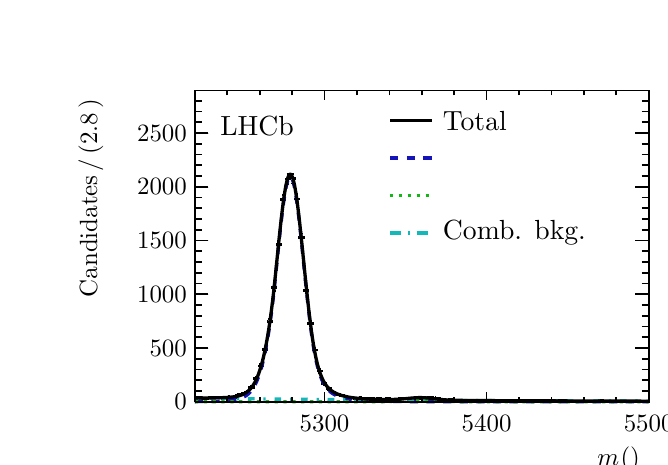
\begin{tikzpicture}[scale=0.38]
\pgfdeclareplotmark{cross} {
\pgfpathmoveto{\pgfpoint{-0.3\pgfplotmarksize}{\pgfplotmarksize}}
\pgfpathlineto{\pgfpoint{+0.3\pgfplotmarksize}{\pgfplotmarksize}}
\pgfpathlineto{\pgfpoint{+0.3\pgfplotmarksize}{0.3\pgfplotmarksize}}
\pgfpathlineto{\pgfpoint{+1\pgfplotmarksize}{0.3\pgfplotmarksize}}
\pgfpathlineto{\pgfpoint{+1\pgfplotmarksize}{-0.3\pgfplotmarksize}}
\pgfpathlineto{\pgfpoint{+0.3\pgfplotmarksize}{-0.3\pgfplotmarksize}}
\pgfpathlineto{\pgfpoint{+0.3\pgfplotmarksize}{-1.\pgfplotmarksize}}
\pgfpathlineto{\pgfpoint{-0.3\pgfplotmarksize}{-1.\pgfplotmarksize}}
\pgfpathlineto{\pgfpoint{-0.3\pgfplotmarksize}{-0.3\pgfplotmarksize}}
\pgfpathlineto{\pgfpoint{-1.\pgfplotmarksize}{-0.3\pgfplotmarksize}}
\pgfpathlineto{\pgfpoint{-1.\pgfplotmarksize}{0.3\pgfplotmarksize}}
\pgfpathlineto{\pgfpoint{-0.3\pgfplotmarksize}{0.3\pgfplotmarksize}}
\pgfpathclose
\pgfusepathqstroke
}
\pgfdeclareplotmark{cross*} {
\pgfpathmoveto{\pgfpoint{-0.3\pgfplotmarksize}{\pgfplotmarksize}}
\pgfpathlineto{\pgfpoint{+0.3\pgfplotmarksize}{\pgfplotmarksize}}
\pgfpathlineto{\pgfpoint{+0.3\pgfplotmarksize}{0.3\pgfplotmarksize}}
\pgfpathlineto{\pgfpoint{+1\pgfplotmarksize}{0.3\pgfplotmarksize}}
\pgfpathlineto{\pgfpoint{+1\pgfplotmarksize}{-0.3\pgfplotmarksize}}
\pgfpathlineto{\pgfpoint{+0.3\pgfplotmarksize}{-0.3\pgfplotmarksize}}
\pgfpathlineto{\pgfpoint{+0.3\pgfplotmarksize}{-1.\pgfplotmarksize}}
\pgfpathlineto{\pgfpoint{-0.3\pgfplotmarksize}{-1.\pgfplotmarksize}}
\pgfpathlineto{\pgfpoint{-0.3\pgfplotmarksize}{-0.3\pgfplotmarksize}}
\pgfpathlineto{\pgfpoint{-1.\pgfplotmarksize}{-0.3\pgfplotmarksize}}
\pgfpathlineto{\pgfpoint{-1.\pgfplotmarksize}{0.3\pgfplotmarksize}}
\pgfpathlineto{\pgfpoint{-0.3\pgfplotmarksize}{0.3\pgfplotmarksize}}
\pgfpathclose
\pgfusepathqfillstroke
}
\pgfdeclareplotmark{newstar} {
\pgfpathmoveto{\pgfqpoint{0pt}{\pgfplotmarksize}}
\pgfpathlineto{\pgfqpointpolar{44}{0.5\pgfplotmarksize}}
\pgfpathlineto{\pgfqpointpolar{18}{\pgfplotmarksize}}
\pgfpathlineto{\pgfqpointpolar{-20}{0.5\pgfplotmarksize}}
\pgfpathlineto{\pgfqpointpolar{-54}{\pgfplotmarksize}}
\pgfpathlineto{\pgfqpointpolar{-90}{0.5\pgfplotmarksize}}
\pgfpathlineto{\pgfqpointpolar{234}{\pgfplotmarksize}}
\pgfpathlineto{\pgfqpointpolar{198}{0.5\pgfplotmarksize}}
\pgfpathlineto{\pgfqpointpolar{162}{\pgfplotmarksize}}
\pgfpathlineto{\pgfqpointpolar{134}{0.5\pgfplotmarksize}}
\pgfpathclose
\pgfusepathqstroke
}
\pgfdeclareplotmark{newstar*} {
\pgfpathmoveto{\pgfqpoint{0pt}{\pgfplotmarksize}}
\pgfpathlineto{\pgfqpointpolar{44}{0.5\pgfplotmarksize}}
\pgfpathlineto{\pgfqpointpolar{18}{\pgfplotmarksize}}
\pgfpathlineto{\pgfqpointpolar{-20}{0.5\pgfplotmarksize}}
\pgfpathlineto{\pgfqpointpolar{-54}{\pgfplotmarksize}}
\pgfpathlineto{\pgfqpointpolar{-90}{0.5\pgfplotmarksize}}
\pgfpathlineto{\pgfqpointpolar{234}{\pgfplotmarksize}}
\pgfpathlineto{\pgfqpointpolar{198}{0.5\pgfplotmarksize}}
\pgfpathlineto{\pgfqpointpolar{162}{\pgfplotmarksize}}
\pgfpathlineto{\pgfqpointpolar{134}{0.5\pgfplotmarksize}}
\pgfpathclose
\pgfusepathqfillstroke
}
\definecolor{c}{rgb}{1,1,1};
\draw [color=c, fill=c] (0.4,0) rectangle (19.6,13.1687);
\draw [color=c, fill=c] (3.472,2.107) rectangle (18.64,12.5103);
\definecolor{c}{rgb}{0,0,0};
\draw [c,line width=0.6] (3.472,2.107) -- (3.472,12.5103) -- (18.64,12.5103) -- (18.64,2.107) -- (3.472,2.107);
\definecolor{c}{rgb}{1,1,1};
\draw [color=c, fill=c] (3.472,2.107) rectangle (18.64,12.5103);
\definecolor{c}{rgb}{0,0,0};
\draw [c,line width=0.6] (3.472,2.107) -- (3.472,12.5103) -- (18.64,12.5103) -- (18.64,2.107) -- (3.472,2.107);
\draw [c,line width=0.6] (3.472,2.107) -- (18.64,2.107);
%\draw [anchor= east] (18.64,0.665812) node[scale=2.08555, color=c, rotate=0]{$\it{m_{D_{s} D}} (MeV/c^{2})$};
\draw [anchor= east] (18.64,0.2) node[scale=0.9, color=c, rotate=0]{${m_{\Ds \Dm}} ({\mevcc})$};
\draw [c,line width=0.6] (7.80571,2.4191) -- (7.80571,2.107);
\draw [c,line width=0.6] (8.88914,2.26305) -- (8.88914,2.107);
\draw [c,line width=0.6] (9.97257,2.26305) -- (9.97257,2.107);
\draw [c,line width=0.6] (11.056,2.26305) -- (11.056,2.107);
\draw [c,line width=0.6] (12.1394,2.26305) -- (12.1394,2.107);
\draw [c,line width=0.6] (13.2229,2.4191) -- (13.2229,2.107);
\draw [c,line width=0.6] (14.3063,2.26305) -- (14.3063,2.107);
\draw [c,line width=0.6] (15.3897,2.26305) -- (15.3897,2.107);
\draw [c,line width=0.6] (16.4731,2.26305) -- (16.4731,2.107);
\draw [c,line width=0.6] (17.5566,2.26305) -- (17.5566,2.107);
\draw [c,line width=0.6] (18.64,2.4191) -- (18.64,2.107);
\draw [c,line width=0.6] (7.80571,2.4191) -- (7.80571,2.107);
\draw [c,line width=0.6] (6.72229,2.26305) -- (6.72229,2.107);
\draw [c,line width=0.6] (5.63886,2.26305) -- (5.63886,2.107);
\draw [c,line width=0.6] (4.55543,2.26305) -- (4.55543,2.107);
\draw [anchor=base] (7.80571,1.1) node[scale=0.9, color=c, rotate=0]{$5300$};
\draw [anchor=base] (13.2229,1.1) node[scale=0.9, color=c, rotate=0]{$5400$};
\draw [anchor=base] (18.64,1.1) node[scale=0.9, color=c, rotate=0]{$5500$};
\draw [c,line width=0.6] (3.472,12.5103) -- (18.64,12.5103);
\draw [c,line width=0.6] (7.80571,12.1982) -- (7.80571,12.5103);
\draw [c,line width=0.6] (8.88914,12.3543) -- (8.88914,12.5103);
\draw [c,line width=0.6] (9.97257,12.3543) -- (9.97257,12.5103);
\draw [c,line width=0.6] (11.056,12.3543) -- (11.056,12.5103);
\draw [c,line width=0.6] (12.1394,12.3543) -- (12.1394,12.5103);
\draw [c,line width=0.6] (13.2229,12.1982) -- (13.2229,12.5103);
\draw [c,line width=0.6] (14.3063,12.3543) -- (14.3063,12.5103);
\draw [c,line width=0.6] (15.3897,12.3543) -- (15.3897,12.5103);
\draw [c,line width=0.6] (16.4731,12.3543) -- (16.4731,12.5103);
\draw [c,line width=0.6] (17.5566,12.3543) -- (17.5566,12.5103);
\draw [c,line width=0.6] (18.64,12.1982) -- (18.64,12.5103);
\draw [c,line width=0.6] (7.80571,12.1982) -- (7.80571,12.5103);
\draw [c,line width=0.6] (6.72229,12.3543) -- (6.72229,12.5103);
\draw [c,line width=0.6] (5.63886,12.3543) -- (5.63886,12.5103);
\draw [c,line width=0.6] (4.55543,12.3543) -- (4.55543,12.5103);
\draw [c,line width=0.6] (3.472,2.107) -- (3.472,12.5103);
%\draw [anchor= east] (1.03898,12.5103) node[scale=1.93658, color=c, rotate=90]{$Candidates / ( 2.8 MeV/c^{2} )$};
\draw [anchor= east] (0.,12.5103) node[scale=0.9, color=c, rotate=90]{Candidates\,/\,(2.8\,\mevcc)};
\draw [c,line width=0.6] (3.92704,2.107) -- (3.472,2.107);
\draw [c,line width=0.6] (3.69952,2.46615) -- (3.472,2.46615);
\draw [c,line width=0.6] (3.69952,2.82531) -- (3.472,2.82531);
\draw [c,line width=0.6] (3.69952,3.18446) -- (3.472,3.18446);
\draw [c,line width=0.6] (3.69952,3.54361) -- (3.472,3.54361);
\draw [c,line width=0.6] (3.92704,3.90277) -- (3.472,3.90277);
\draw [c,line width=0.6] (3.69952,4.26192) -- (3.472,4.26192);
\draw [c,line width=0.6] (3.69952,4.62107) -- (3.472,4.62107);
\draw [c,line width=0.6] (3.69952,4.98023) -- (3.472,4.98023);
\draw [c,line width=0.6] (3.69952,5.33938) -- (3.472,5.33938);
\draw [c,line width=0.6] (3.92704,5.69853) -- (3.472,5.69853);
\draw [c,line width=0.6] (3.69952,6.05769) -- (3.472,6.05769);
\draw [c,line width=0.6] (3.69952,6.41684) -- (3.472,6.41684);
\draw [c,line width=0.6] (3.69952,6.776) -- (3.472,6.776);
\draw [c,line width=0.6] (3.69952,7.13515) -- (3.472,7.13515);
\draw [c,line width=0.6] (3.92704,7.4943) -- (3.472,7.4943);
\draw [c,line width=0.6] (3.69952,7.85346) -- (3.472,7.85346);
\draw [c,line width=0.6] (3.69952,8.21261) -- (3.472,8.21261);
\draw [c,line width=0.6] (3.69952,8.57176) -- (3.472,8.57176);
\draw [c,line width=0.6] (3.69952,8.93092) -- (3.472,8.93092);
\draw [c,line width=0.6] (3.92704,9.29007) -- (3.472,9.29007);
\draw [c,line width=0.6] (3.69952,9.64922) -- (3.472,9.64922);
\draw [c,line width=0.6] (3.69952,10.0084) -- (3.472,10.0084);
\draw [c,line width=0.6] (3.69952,10.3675) -- (3.472,10.3675);
\draw [c,line width=0.6] (3.69952,10.7267) -- (3.472,10.7267);
\draw [c,line width=0.6] (3.92704,11.0858) -- (3.472,11.0858);
\draw [c,line width=0.6] (3.92704,11.0858) -- (3.472,11.0858);
\draw [c,line width=0.6] (3.69952,11.445) -- (3.472,11.445);
\draw [c,line width=0.6] (3.69952,11.8041) -- (3.472,11.8041);
\draw [c,line width=0.6] (3.69952,12.1633) -- (3.472,12.1633);
\draw [anchor= east] (3.5,2.107) node[scale=0.9, color=c, rotate=0]{$0$};
\draw [anchor= east] (3.5,3.90277) node[scale=0.9, color=c, rotate=0]{$500$};
\draw [anchor= east] (3.5,5.69853) node[scale=0.9, color=c, rotate=0]{$1000$};
\draw [anchor= east] (3.5,7.4943) node[scale=0.9, color=c, rotate=0]{$1500$};
\draw [anchor= east] (3.5,9.29007) node[scale=0.9, color=c, rotate=0]{$2000$};
\draw [anchor= east] (3.5,11.0858) node[scale=0.9, color=c, rotate=0]{$2500$};
\draw [c,line width=0.6] (18.64,2.107) -- (18.64,12.5103);
\draw [c,line width=0.6] (18.185,2.107) -- (18.64,2.107);
\draw [c,line width=0.6] (18.4125,2.46615) -- (18.64,2.46615);
\draw [c,line width=0.6] (18.4125,2.82531) -- (18.64,2.82531);
\draw [c,line width=0.6] (18.4125,3.18446) -- (18.64,3.18446);
\draw [c,line width=0.6] (18.4125,3.54361) -- (18.64,3.54361);
\draw [c,line width=0.6] (18.185,3.90277) -- (18.64,3.90277);
\draw [c,line width=0.6] (18.4125,4.26192) -- (18.64,4.26192);
\draw [c,line width=0.6] (18.4125,4.62107) -- (18.64,4.62107);
\draw [c,line width=0.6] (18.4125,4.98023) -- (18.64,4.98023);
\draw [c,line width=0.6] (18.4125,5.33938) -- (18.64,5.33938);
\draw [c,line width=0.6] (18.185,5.69853) -- (18.64,5.69853);
\draw [c,line width=0.6] (18.4125,6.05769) -- (18.64,6.05769);
\draw [c,line width=0.6] (18.4125,6.41684) -- (18.64,6.41684);
\draw [c,line width=0.6] (18.4125,6.776) -- (18.64,6.776);
\draw [c,line width=0.6] (18.4125,7.13515) -- (18.64,7.13515);
\draw [c,line width=0.6] (18.185,7.4943) -- (18.64,7.4943);
\draw [c,line width=0.6] (18.4125,7.85346) -- (18.64,7.85346);
\draw [c,line width=0.6] (18.4125,8.21261) -- (18.64,8.21261);
\draw [c,line width=0.6] (18.4125,8.57176) -- (18.64,8.57176);
\draw [c,line width=0.6] (18.4125,8.93092) -- (18.64,8.93092);
\draw [c,line width=0.6] (18.185,9.29007) -- (18.64,9.29007);
\draw [c,line width=0.6] (18.4125,9.64922) -- (18.64,9.64922);
\draw [c,line width=0.6] (18.4125,10.0084) -- (18.64,10.0084);
\draw [c,line width=0.6] (18.4125,10.3675) -- (18.64,10.3675);
\draw [c,line width=0.6] (18.4125,10.7267) -- (18.64,10.7267);
\draw [c,line width=0.6] (18.185,11.0858) -- (18.64,11.0858);
\draw [c,line width=0.6] (18.185,11.0858) -- (18.64,11.0858);
\draw [c,line width=0.6] (18.4125,11.445) -- (18.64,11.445);
\draw [c,line width=0.6] (18.4125,11.8041) -- (18.64,11.8041);
\draw [c,line width=0.6] (18.4125,12.1633) -- (18.64,12.1633);
\draw [c,line width=0.6] (3.54784,2.21475) -- (3.472,2.21475);
\draw [c,line width=0.6] (3.472,2.1701) -- (3.472,2.25939);
\draw [c,line width=0.6] (3.54784,2.21475) -- (3.62368,2.21475);
\draw [c,line width=0.6] (3.62368,2.1701) -- (3.62368,2.25939);
\draw [c,line width=0.6] (3.54784,2.21475) -- (3.54784,2.23823);
\draw [c,line width=0.6] (3.5032,2.23823) -- (3.59248,2.23823);
\draw [c,line width=0.6] (3.54784,2.21475) -- (3.54784,2.19518);
\draw [c,line width=0.6] (3.5032,2.19518) -- (3.59248,2.19518);
\draw [c,line width=0.6] (3.69952,2.21834) -- (3.62368,2.21834);
\draw [c,line width=0.6] (3.62368,2.17369) -- (3.62368,2.26298);
\draw [c,line width=0.6] (3.69952,2.21834) -- (3.77536,2.21834);
\draw [c,line width=0.6] (3.77536,2.17369) -- (3.77536,2.26298);
\draw [c,line width=0.6] (3.69952,2.21834) -- (3.69952,2.24214);
\draw [c,line width=0.6] (3.65488,2.24214) -- (3.74416,2.24214);
\draw [c,line width=0.6] (3.69952,2.21834) -- (3.69952,2.19845);
\draw [c,line width=0.6] (3.65488,2.19845) -- (3.74416,2.19845);
\draw [c,line width=0.6] (3.8512,2.21115) -- (3.77536,2.21115);
\draw [c,line width=0.6] (3.77536,2.16651) -- (3.77536,2.2558);
\draw [c,line width=0.6] (3.8512,2.21115) -- (3.92704,2.21115);
\draw [c,line width=0.6] (3.92704,2.16651) -- (3.92704,2.2558);
\draw [c,line width=0.6] (3.8512,2.21115) -- (3.8512,2.23431);
\draw [c,line width=0.6] (3.80656,2.23431) -- (3.89584,2.23431);
\draw [c,line width=0.6] (3.8512,2.21115) -- (3.8512,2.19193);
\draw [c,line width=0.6] (3.80656,2.19193) -- (3.89584,2.19193);
\draw [c,line width=0.6] (4.00288,2.24348) -- (3.92704,2.24348);
\draw [c,line width=0.6] (3.92704,2.19884) -- (3.92704,2.28812);
\draw [c,line width=0.6] (4.00288,2.24348) -- (4.07872,2.24348);
\draw [c,line width=0.6] (4.07872,2.19884) -- (4.07872,2.28812);
\draw [c,line width=0.6] (4.00288,2.24348) -- (4.00288,2.2694);
\draw [c,line width=0.6] (3.95824,2.2694) -- (4.04752,2.2694);
\draw [c,line width=0.6] (4.00288,2.24348) -- (4.00288,2.22144);
\draw [c,line width=0.6] (3.95824,2.22144) -- (4.04752,2.22144);
\draw [c,line width=0.6] (4.15456,2.24348) -- (4.07872,2.24348);
\draw [c,line width=0.6] (4.07872,2.19884) -- (4.07872,2.28812);
\draw [c,line width=0.6] (4.15456,2.24348) -- (4.2304,2.24348);
\draw [c,line width=0.6] (4.2304,2.19884) -- (4.2304,2.28812);
\draw [c,line width=0.6] (4.15456,2.24348) -- (4.15456,2.2694);
\draw [c,line width=0.6] (4.10992,2.2694) -- (4.1992,2.2694);
\draw [c,line width=0.6] (4.15456,2.24348) -- (4.15456,2.22144);
\draw [c,line width=0.6] (4.10992,2.22144) -- (4.1992,2.22144);
\draw [c,line width=0.6] (4.30624,2.23989) -- (4.2304,2.23989);
\draw [c,line width=0.6] (4.2304,2.19524) -- (4.2304,2.28453);
\draw [c,line width=0.6] (4.30624,2.23989) -- (4.38208,2.23989);
\draw [c,line width=0.6] (4.38208,2.19524) -- (4.38208,2.28453);
\draw [c,line width=0.6] (4.30624,2.23989) -- (4.30624,2.26552);
\draw [c,line width=0.6] (4.2616,2.26552) -- (4.35088,2.26552);
\draw [c,line width=0.6] (4.30624,2.23989) -- (4.30624,2.21814);
\draw [c,line width=0.6] (4.2616,2.21814) -- (4.35088,2.21814);
\draw [c,line width=0.6] (4.45792,2.21475) -- (4.38208,2.21475);
\draw [c,line width=0.6] (4.38208,2.1701) -- (4.38208,2.25939);
\draw [c,line width=0.6] (4.45792,2.21475) -- (4.53376,2.21475);
\draw [c,line width=0.6] (4.53376,2.1701) -- (4.53376,2.25939);
\draw [c,line width=0.6] (4.45792,2.21475) -- (4.45792,2.23823);
\draw [c,line width=0.6] (4.41328,2.23823) -- (4.50256,2.23823);
\draw [c,line width=0.6] (4.45792,2.21475) -- (4.45792,2.19518);
\draw [c,line width=0.6] (4.41328,2.19518) -- (4.50256,2.19518);
\draw [c,line width=0.6] (4.6096,2.26503) -- (4.53376,2.26503);
\draw [c,line width=0.6] (4.53376,2.22038) -- (4.53376,2.30967);
\draw [c,line width=0.6] (4.6096,2.26503) -- (4.68544,2.26503);
\draw [c,line width=0.6] (4.68544,2.22038) -- (4.68544,2.30967);
\draw [c,line width=0.6] (4.6096,2.26503) -- (4.6096,2.29262);
\draw [c,line width=0.6] (4.56496,2.29262) -- (4.65424,2.29262);
\draw [c,line width=0.6] (4.6096,2.26503) -- (4.6096,2.24129);
\draw [c,line width=0.6] (4.56496,2.24129) -- (4.65424,2.24129);
\draw [c,line width=0.6] (4.76128,2.24707) -- (4.68544,2.24707);
\draw [c,line width=0.6] (4.68544,2.20243) -- (4.68544,2.29171);
\draw [c,line width=0.6] (4.76128,2.24707) -- (4.83712,2.24707);
\draw [c,line width=0.6] (4.83712,2.20243) -- (4.83712,2.29171);
\draw [c,line width=0.6] (4.76128,2.24707) -- (4.76128,2.27328);
\draw [c,line width=0.6] (4.71664,2.27328) -- (4.80592,2.27328);
\draw [c,line width=0.6] (4.76128,2.24707) -- (4.76128,2.22474);
\draw [c,line width=0.6] (4.71664,2.22474) -- (4.80592,2.22474);
\draw [c,line width=0.6] (4.91296,2.32608) -- (4.83712,2.32608);
\draw [c,line width=0.6] (4.83712,2.28144) -- (4.83712,2.37073);
\draw [c,line width=0.6] (4.91296,2.32608) -- (4.9888,2.32608);
\draw [c,line width=0.6] (4.9888,2.28144) -- (4.9888,2.37073);
\draw [c,line width=0.6] (4.91296,2.32608) -- (4.91296,2.35788);
\draw [c,line width=0.6] (4.86832,2.35788) -- (4.9576,2.35788);
\draw [c,line width=0.6] (4.91296,2.32608) -- (4.91296,2.29811);
\draw [c,line width=0.6] (4.86832,2.29811) -- (4.9576,2.29811);
\draw [c,line width=0.6] (5.06464,2.36559) -- (4.9888,2.36559);
\draw [c,line width=0.6] (4.9888,2.32095) -- (4.9888,2.41023);
\draw [c,line width=0.6] (5.06464,2.36559) -- (5.14048,2.36559);
\draw [c,line width=0.6] (5.14048,2.32095) -- (5.14048,2.41023);
\draw [c,line width=0.6] (5.06464,2.36559) -- (5.06464,2.3998);
\draw [c,line width=0.6] (5.02,2.3998) -- (5.10928,2.3998);
\draw [c,line width=0.6] (5.06464,2.36559) -- (5.06464,2.33519);
\draw [c,line width=0.6] (5.02,2.33519) -- (5.10928,2.33519);
\draw [c,line width=0.6] (5.21632,2.42665) -- (5.14048,2.42665);
\draw [c,line width=0.6] (5.14048,2.382) -- (5.14048,2.47129);
\draw [c,line width=0.6] (5.21632,2.42665) -- (5.29216,2.42665);
\draw [c,line width=0.6] (5.29216,2.382) -- (5.29216,2.47129);
\draw [c,line width=0.6] (5.21632,2.42665) -- (5.21632,2.46425);
\draw [c,line width=0.6] (5.17168,2.46425) -- (5.26096,2.46425);
\draw [c,line width=0.6] (5.21632,2.42665) -- (5.21632,2.39283);
\draw [c,line width=0.6] (5.17168,2.39283) -- (5.26096,2.39283);
\draw [c,line width=0.6] (5.368,2.59186) -- (5.29216,2.59186);
\draw [c,line width=0.6] (5.29216,2.54721) -- (5.29216,2.6365);
\draw [c,line width=0.6] (5.368,2.59186) -- (5.44384,2.59186);
\draw [c,line width=0.6] (5.44384,2.54721) -- (5.44384,2.6365);
\draw [c,line width=0.6] (5.368,2.59186) -- (5.368,2.63542);
\draw [c,line width=0.6] (5.32336,2.63542) -- (5.41264,2.63542);
\draw [c,line width=0.6] (5.368,2.59186) -- (5.368,2.55188);
\draw [c,line width=0.6] (5.32336,2.55188) -- (5.41264,2.55188);
\draw [c,line width=0.6] (5.51968,2.88995) -- (5.44384,2.88995);
\draw [c,line width=0.6] (5.44384,2.84531) -- (5.44384,2.9346);
\draw [c,line width=0.6] (5.51968,2.88995) -- (5.59552,2.88995);
\draw [c,line width=0.6] (5.59552,2.84531) -- (5.59552,2.9346);
\draw [c,line width=0.6] (5.51968,2.88995) -- (5.51968,2.94481);
\draw [c,line width=0.6] (5.47504,2.94481) -- (5.56432,2.94481);
\draw [c,line width=0.6] (5.51968,2.88995) -- (5.51968,2.83869);
\draw [c,line width=0.6] (5.47504,2.83869) -- (5.56432,2.83869);
\draw [c,line width=0.6] (5.67136,3.29939) -- (5.59552,3.29939);
\draw [c,line width=0.6] (5.59552,3.25475) -- (5.59552,3.34403);
\draw [c,line width=0.6] (5.67136,3.29939) -- (5.7472,3.29939);
\draw [c,line width=0.6] (5.7472,3.25475) -- (5.7472,3.34403);
\draw [c,line width=0.6] (5.67136,3.29939) -- (5.67136,3.36665);
\draw [c,line width=0.6] (5.62672,3.36665) -- (5.716,3.36665);
\draw [c,line width=0.6] (5.67136,3.29939) -- (5.67136,3.23572);
\draw [c,line width=0.6] (5.62672,3.23572) -- (5.716,3.23572);
\draw [c,line width=0.6] (5.82304,3.85249) -- (5.7472,3.85249);
\draw [c,line width=0.6] (5.7472,3.80784) -- (5.7472,3.89713);
\draw [c,line width=0.6] (5.82304,3.85249) -- (5.89888,3.85249);
\draw [c,line width=0.6] (5.89888,3.80784) -- (5.89888,3.89713);
\draw [c,line width=0.6] (5.82304,3.85249) -- (5.82304,3.93348);
\draw [c,line width=0.6] (5.7784,3.93348) -- (5.86768,3.93348);
\draw [c,line width=0.6] (5.82304,3.85249) -- (5.82304,3.77508);
\draw [c,line width=0.6] (5.7784,3.77508) -- (5.86768,3.77508);
\draw [c,line width=0.6] (5.97472,4.7791) -- (5.89888,4.7791);
\draw [c,line width=0.6] (5.89888,4.73446) -- (5.89888,4.82374);
\draw [c,line width=0.6] (5.97472,4.7791) -- (6.05056,4.7791);
\draw [c,line width=0.6] (6.05056,4.73446) -- (6.05056,4.82374);
\draw [c,line width=0.6] (5.97472,4.7791) -- (5.97472,4.87888);
\draw [c,line width=0.6] (5.93008,4.87888) -- (6.01936,4.87888);
\draw [c,line width=0.6] (5.97472,4.7791) -- (5.97472,4.68292);
\draw [c,line width=0.6] (5.93008,4.68292) -- (6.01936,4.68292);
\draw [c,line width=0.6] (6.1264,5.91762) -- (6.05056,5.91762);
\draw [c,line width=0.6] (6.05056,5.87298) -- (6.05056,5.96226);
\draw [c,line width=0.6] (6.1264,5.91762) -- (6.20224,5.91762);
\draw [c,line width=0.6] (6.20224,5.87298) -- (6.20224,5.96226);
\draw [c,line width=0.6] (6.1264,5.91762) -- (6.1264,6.03642);
\draw [c,line width=0.6] (6.08176,6.03642) -- (6.17104,6.03642);
\draw [c,line width=0.6] (6.1264,5.91762) -- (6.1264,5.80241);
\draw [c,line width=0.6] (6.08176,5.80241) -- (6.17104,5.80241);
\draw [c,line width=0.6] (6.27808,7.35423) -- (6.20224,7.35423);
\draw [c,line width=0.6] (6.20224,7.30959) -- (6.20224,7.39888);
\draw [c,line width=0.6] (6.27808,7.35423) -- (6.35392,7.35423);
\draw [c,line width=0.6] (6.35392,7.30959) -- (6.35392,7.39888);
\draw [c,line width=0.6] (6.27808,7.35423) -- (6.27808,7.49332);
\draw [c,line width=0.6] (6.23344,7.49332) -- (6.32272,7.49332);
\draw [c,line width=0.6] (6.27808,7.35423) -- (6.27808,7.21874);
\draw [c,line width=0.6] (6.23344,7.21874) -- (6.32272,7.21874);
\draw [c,line width=0.6] (6.42976,8.86627) -- (6.35392,8.86627);
\draw [c,line width=0.6] (6.35392,8.82163) -- (6.35392,8.91091);
\draw [c,line width=0.6] (6.42976,8.86627) -- (6.5056,8.86627);
\draw [c,line width=0.6] (6.5056,8.82163) -- (6.5056,8.91091);
\draw [c,line width=0.6] (6.42976,8.86627) -- (6.42976,9.02388);
\draw [c,line width=0.6] (6.38512,9.02388) -- (6.4744,9.02388);
\draw [c,line width=0.6] (6.42976,8.86627) -- (6.42976,8.71225);
\draw [c,line width=0.6] (6.38512,8.71225) -- (6.4744,8.71225);
\draw [c,line width=0.6] (6.58144,9.55584) -- (6.5056,9.55584);
\draw [c,line width=0.6] (6.5056,9.5112) -- (6.5056,9.60049);
\draw [c,line width=0.6] (6.58144,9.55584) -- (6.65728,9.55584);
\draw [c,line width=0.6] (6.65728,9.5112) -- (6.65728,9.60049);
\draw [c,line width=0.6] (6.58144,9.55584) -- (6.58144,9.72121);
\draw [c,line width=0.6] (6.5368,9.72121) -- (6.62608,9.72121);
\draw [c,line width=0.6] (6.58144,9.55584) -- (6.58144,9.39407);
\draw [c,line width=0.6] (6.5368,9.39407) -- (6.62608,9.39407);
\draw [c,line width=0.6] (6.73312,9.56303) -- (6.65728,9.56303);
\draw [c,line width=0.6] (6.65728,9.51838) -- (6.65728,9.60767);
\draw [c,line width=0.6] (6.73312,9.56303) -- (6.80896,9.56303);
\draw [c,line width=0.6] (6.80896,9.51838) -- (6.80896,9.60767);
\draw [c,line width=0.6] (6.73312,9.56303) -- (6.73312,9.72847);
\draw [c,line width=0.6] (6.68848,9.72847) -- (6.77776,9.72847);
\draw [c,line width=0.6] (6.73312,9.56303) -- (6.73312,9.40117);
\draw [c,line width=0.6] (6.68848,9.40117) -- (6.77776,9.40117);
\draw [c,line width=0.6] (6.8848,8.88064) -- (6.80896,8.88064);
\draw [c,line width=0.6] (6.80896,8.83599) -- (6.80896,8.92528);
\draw [c,line width=0.6] (6.8848,8.88064) -- (6.96064,8.88064);
\draw [c,line width=0.6] (6.96064,8.83599) -- (6.96064,8.92528);
\draw [c,line width=0.6] (6.8848,8.88064) -- (6.8848,9.03841);
\draw [c,line width=0.6] (6.84016,9.03841) -- (6.92944,9.03841);
\draw [c,line width=0.6] (6.8848,8.88064) -- (6.8848,8.72645);
\draw [c,line width=0.6] (6.84016,8.72645) -- (6.92944,8.72645);
\draw [c,line width=0.6] (7.03648,7.58768) -- (6.96064,7.58768);
\draw [c,line width=0.6] (6.96064,7.54304) -- (6.96064,7.63233);
\draw [c,line width=0.6] (7.03648,7.58768) -- (7.11232,7.58768);
\draw [c,line width=0.6] (7.11232,7.54304) -- (7.11232,7.63233);
\draw [c,line width=0.6] (7.03648,7.58768) -- (7.03648,7.72979);
\draw [c,line width=0.6] (6.99184,7.72979) -- (7.08112,7.72979);
\draw [c,line width=0.6] (7.03648,7.58768) -- (7.03648,7.44917);
\draw [c,line width=0.6] (6.99184,7.44917) -- (7.08112,7.44917);
\draw [c,line width=0.6] (7.18816,5.83501) -- (7.11232,5.83501);
\draw [c,line width=0.6] (7.11232,5.79037) -- (7.11232,5.87966);
\draw [c,line width=0.6] (7.18816,5.83501) -- (7.264,5.83501);
\draw [c,line width=0.6] (7.264,5.79037) -- (7.264,5.87966);
\draw [c,line width=0.6] (7.18816,5.83501) -- (7.18816,5.95254);
\draw [c,line width=0.6] (7.14352,5.95254) -- (7.2328,5.95254);
\draw [c,line width=0.6] (7.18816,5.83501) -- (7.18816,5.72108);
\draw [c,line width=0.6] (7.14352,5.72108) -- (7.2328,5.72108);
\draw [c,line width=0.6] (7.33984,4.72164) -- (7.264,4.72164);
\draw [c,line width=0.6] (7.264,4.67699) -- (7.264,4.76628);
\draw [c,line width=0.6] (7.33984,4.72164) -- (7.41568,4.72164);
\draw [c,line width=0.6] (7.41568,4.67699) -- (7.41568,4.76628);
\draw [c,line width=0.6] (7.33984,4.72164) -- (7.33984,4.82035);
\draw [c,line width=0.6] (7.2952,4.82035) -- (7.38448,4.82035);
\draw [c,line width=0.6] (7.33984,4.72164) -- (7.33984,4.62651);
\draw [c,line width=0.6] (7.2952,4.62651) -- (7.38448,4.62651);
\draw [c,line width=0.6] (7.49152,3.83453) -- (7.41568,3.83453);
\draw [c,line width=0.6] (7.41568,3.78989) -- (7.41568,3.87917);
\draw [c,line width=0.6] (7.49152,3.83453) -- (7.56736,3.83453);
\draw [c,line width=0.6] (7.56736,3.78989) -- (7.56736,3.87917);
\draw [c,line width=0.6] (7.49152,3.83453) -- (7.49152,3.91511);
\draw [c,line width=0.6] (7.44688,3.91511) -- (7.53616,3.91511);
\draw [c,line width=0.6] (7.49152,3.83453) -- (7.49152,3.75754);
\draw [c,line width=0.6] (7.44688,3.75754) -- (7.53616,3.75754);
\draw [c,line width=0.6] (7.6432,3.13418) -- (7.56736,3.13418);
\draw [c,line width=0.6] (7.56736,3.08954) -- (7.56736,3.17882);
\draw [c,line width=0.6] (7.6432,3.13418) -- (7.71904,3.13418);
\draw [c,line width=0.6] (7.71904,3.08954) -- (7.71904,3.17882);
\draw [c,line width=0.6] (7.6432,3.13418) -- (7.6432,3.19674);
\draw [c,line width=0.6] (7.59856,3.19674) -- (7.68784,3.19674);
\draw [c,line width=0.6] (7.6432,3.13418) -- (7.6432,3.07521);
\draw [c,line width=0.6] (7.59856,3.07521) -- (7.68784,3.07521);
\draw [c,line width=0.6] (7.79488,2.70679) -- (7.71904,2.70679);
\draw [c,line width=0.6] (7.71904,2.66214) -- (7.71904,2.75143);
\draw [c,line width=0.6] (7.79488,2.70679) -- (7.87072,2.70679);
\draw [c,line width=0.6] (7.87072,2.66214) -- (7.87072,2.75143);
\draw [c,line width=0.6] (7.79488,2.70679) -- (7.79488,2.75503);
\draw [c,line width=0.6] (7.75024,2.75503) -- (7.83952,2.75503);
\draw [c,line width=0.6] (7.79488,2.70679) -- (7.79488,2.66213);
\draw [c,line width=0.6] (7.75024,2.66213) -- (7.83952,2.66213);
\draw [c,line width=0.6] (7.94656,2.53798) -- (7.87072,2.53798);
\draw [c,line width=0.6] (7.87072,2.49334) -- (7.87072,2.58263);
\draw [c,line width=0.6] (7.94656,2.53798) -- (8.0224,2.53798);
\draw [c,line width=0.6] (8.0224,2.49334) -- (8.0224,2.58263);
\draw [c,line width=0.6] (7.94656,2.53798) -- (7.94656,2.57916);
\draw [c,line width=0.6] (7.90192,2.57916) -- (7.9912,2.57916);
\draw [c,line width=0.6] (7.94656,2.53798) -- (7.94656,2.5004);
\draw [c,line width=0.6] (7.90192,2.5004) -- (7.9912,2.5004);
\draw [c,line width=0.6] (8.09824,2.41228) -- (8.0224,2.41228);
\draw [c,line width=0.6] (8.0224,2.36764) -- (8.0224,2.45692);
\draw [c,line width=0.6] (8.09824,2.41228) -- (8.17408,2.41228);
\draw [c,line width=0.6] (8.17408,2.36764) -- (8.17408,2.45692);
\draw [c,line width=0.6] (8.09824,2.41228) -- (8.09824,2.44911);
\draw [c,line width=0.6] (8.0536,2.44911) -- (8.14288,2.44911);
\draw [c,line width=0.6] (8.09824,2.41228) -- (8.09824,2.37923);
\draw [c,line width=0.6] (8.0536,2.37923) -- (8.14288,2.37923);
\draw [c,line width=0.6] (8.24992,2.34763) -- (8.17408,2.34763);
\draw [c,line width=0.6] (8.17408,2.30299) -- (8.17408,2.39228);
\draw [c,line width=0.6] (8.24992,2.34763) -- (8.32576,2.34763);
\draw [c,line width=0.6] (8.32576,2.30299) -- (8.32576,2.39228);
\draw [c,line width=0.6] (8.24992,2.34763) -- (8.24992,2.38077);
\draw [c,line width=0.6] (8.20528,2.38077) -- (8.29456,2.38077);
\draw [c,line width=0.6] (8.24992,2.34763) -- (8.24992,2.31831);
\draw [c,line width=0.6] (8.20528,2.31831) -- (8.29456,2.31831);
\draw [c,line width=0.6] (8.4016,2.30453) -- (8.32576,2.30453);
\draw [c,line width=0.6] (8.32576,2.25989) -- (8.32576,2.34918);
\draw [c,line width=0.6] (8.4016,2.30453) -- (8.47744,2.30453);
\draw [c,line width=0.6] (8.47744,2.25989) -- (8.47744,2.34918);
\draw [c,line width=0.6] (8.4016,2.30453) -- (8.4016,2.33492);
\draw [c,line width=0.6] (8.35696,2.33492) -- (8.44624,2.33492);
\draw [c,line width=0.6] (8.4016,2.30453) -- (8.4016,2.27798);
\draw [c,line width=0.6] (8.35696,2.27798) -- (8.44624,2.27798);
\draw [c,line width=0.6] (8.55328,2.2327) -- (8.47744,2.2327);
\draw [c,line width=0.6] (8.47744,2.18806) -- (8.47744,2.27735);
\draw [c,line width=0.6] (8.55328,2.2327) -- (8.62912,2.2327);
\draw [c,line width=0.6] (8.62912,2.18806) -- (8.62912,2.27735);
\draw [c,line width=0.6] (8.55328,2.2327) -- (8.55328,2.25775);
\draw [c,line width=0.6] (8.50864,2.25775) -- (8.59792,2.25775);
\draw [c,line width=0.6] (8.55328,2.2327) -- (8.55328,2.21156);
\draw [c,line width=0.6] (8.50864,2.21156) -- (8.59792,2.21156);
\draw [c,line width=0.6] (8.70496,2.2327) -- (8.62912,2.2327);
\draw [c,line width=0.6] (8.62912,2.18806) -- (8.62912,2.27735);
\draw [c,line width=0.6] (8.70496,2.2327) -- (8.7808,2.2327);
\draw [c,line width=0.6] (8.7808,2.18806) -- (8.7808,2.27735);
\draw [c,line width=0.6] (8.70496,2.2327) -- (8.70496,2.25775);
\draw [c,line width=0.6] (8.66032,2.25775) -- (8.7496,2.25775);
\draw [c,line width=0.6] (8.70496,2.2327) -- (8.70496,2.21156);
\draw [c,line width=0.6] (8.66032,2.21156) -- (8.7496,2.21156);
\draw [c,line width=0.6] (8.85664,2.20038) -- (8.7808,2.20038);
\draw [c,line width=0.6] (8.7808,2.15574) -- (8.7808,2.24502);
\draw [c,line width=0.6] (8.85664,2.20038) -- (8.93248,2.20038);
\draw [c,line width=0.6] (8.93248,2.15574) -- (8.93248,2.24502);
\draw [c,line width=0.6] (8.85664,2.20038) -- (8.85664,2.22252);
\draw [c,line width=0.6] (8.812,2.22252) -- (8.90128,2.22252);
\draw [c,line width=0.6] (8.85664,2.20038) -- (8.85664,2.18219);
\draw [c,line width=0.6] (8.812,2.18219) -- (8.90128,2.18219);
\draw [c,line width=0.6] (9.00832,2.2327) -- (8.93248,2.2327);
\draw [c,line width=0.6] (8.93248,2.18806) -- (8.93248,2.27735);
\draw [c,line width=0.6] (9.00832,2.2327) -- (9.08416,2.2327);
\draw [c,line width=0.6] (9.08416,2.18806) -- (9.08416,2.27735);
\draw [c,line width=0.6] (9.00832,2.2327) -- (9.00832,2.25775);
\draw [c,line width=0.6] (8.96368,2.25775) -- (9.05296,2.25775);
\draw [c,line width=0.6] (9.00832,2.2327) -- (9.00832,2.21156);
\draw [c,line width=0.6] (8.96368,2.21156) -- (9.05296,2.21156);
\draw [c,line width=0.6] (9.16,2.20756) -- (9.08416,2.20756);
\draw [c,line width=0.6] (9.08416,2.16292) -- (9.08416,2.25221);
\draw [c,line width=0.6] (9.16,2.20756) -- (9.23584,2.20756);
\draw [c,line width=0.6] (9.23584,2.16292) -- (9.23584,2.25221);
\draw [c,line width=0.6] (9.16,2.20756) -- (9.16,2.23039);
\draw [c,line width=0.6] (9.11536,2.23039) -- (9.20464,2.23039);
\draw [c,line width=0.6] (9.16,2.20756) -- (9.16,2.18867);
\draw [c,line width=0.6] (9.11536,2.18867) -- (9.20464,2.18867);
\draw [c,line width=0.6] (9.31168,2.22193) -- (9.23584,2.22193);
\draw [c,line width=0.6] (9.23584,2.17729) -- (9.23584,2.26657);
\draw [c,line width=0.6] (9.31168,2.22193) -- (9.38752,2.22193);
\draw [c,line width=0.6] (9.38752,2.17729) -- (9.38752,2.26657);
\draw [c,line width=0.6] (9.31168,2.22193) -- (9.31168,2.24605);
\draw [c,line width=0.6] (9.26704,2.24605) -- (9.35632,2.24605);
\draw [c,line width=0.6] (9.31168,2.22193) -- (9.31168,2.20172);
\draw [c,line width=0.6] (9.26704,2.20172) -- (9.35632,2.20172);
\draw [c,line width=0.6] (9.46336,2.21834) -- (9.38752,2.21834);
\draw [c,line width=0.6] (9.38752,2.17369) -- (9.38752,2.26298);
\draw [c,line width=0.6] (9.46336,2.21834) -- (9.5392,2.21834);
\draw [c,line width=0.6] (9.5392,2.17369) -- (9.5392,2.26298);
\draw [c,line width=0.6] (9.46336,2.21834) -- (9.46336,2.24214);
\draw [c,line width=0.6] (9.41872,2.24214) -- (9.508,2.24214);
\draw [c,line width=0.6] (9.46336,2.21834) -- (9.46336,2.19845);
\draw [c,line width=0.6] (9.41872,2.19845) -- (9.508,2.19845);
\draw [c,line width=0.6] (9.61504,2.22552) -- (9.5392,2.22552);
\draw [c,line width=0.6] (9.5392,2.18088) -- (9.5392,2.27016);
\draw [c,line width=0.6] (9.61504,2.22552) -- (9.69088,2.22552);
\draw [c,line width=0.6] (9.69088,2.18088) -- (9.69088,2.27016);
\draw [c,line width=0.6] (9.61504,2.22552) -- (9.61504,2.24995);
\draw [c,line width=0.6] (9.5704,2.24995) -- (9.65968,2.24995);
\draw [c,line width=0.6] (9.61504,2.22552) -- (9.61504,2.20499);
\draw [c,line width=0.6] (9.5704,2.20499) -- (9.65968,2.20499);
\draw [c,line width=0.6] (9.76672,2.18601) -- (9.69088,2.18601);
\draw [c,line width=0.6] (9.69088,2.14137) -- (9.69088,2.23066);
\draw [c,line width=0.6] (9.76672,2.18601) -- (9.84256,2.18601);
\draw [c,line width=0.6] (9.84256,2.14137) -- (9.84256,2.23066);
\draw [c,line width=0.6] (9.76672,2.18601) -- (9.76672,2.20671);
\draw [c,line width=0.6] (9.72208,2.20671) -- (9.81136,2.20671);
\draw [c,line width=0.6] (9.76672,2.18601) -- (9.76672,2.1693);
\draw [c,line width=0.6] (9.72208,2.1693) -- (9.81136,2.1693);
\draw [c,line width=0.6] (9.9184,2.22193) -- (9.84256,2.22193);
\draw [c,line width=0.6] (9.84256,2.17729) -- (9.84256,2.26657);
\draw [c,line width=0.6] (9.9184,2.22193) -- (9.99424,2.22193);
\draw [c,line width=0.6] (9.99424,2.17729) -- (9.99424,2.26657);
\draw [c,line width=0.6] (9.9184,2.22193) -- (9.9184,2.24605);
\draw [c,line width=0.6] (9.87376,2.24605) -- (9.96304,2.24605);
\draw [c,line width=0.6] (9.9184,2.22193) -- (9.9184,2.20172);
\draw [c,line width=0.6] (9.87376,2.20172) -- (9.96304,2.20172);
\draw [c,line width=0.6] (10.0701,2.18601) -- (9.99424,2.18601);
\draw [c,line width=0.6] (9.99424,2.14137) -- (9.99424,2.23066);
\draw [c,line width=0.6] (10.0701,2.18601) -- (10.1459,2.18601);
\draw [c,line width=0.6] (10.1459,2.14137) -- (10.1459,2.23066);
\draw [c,line width=0.6] (10.0701,2.18601) -- (10.0701,2.20671);
\draw [c,line width=0.6] (10.0254,2.20671) -- (10.1147,2.20671);
\draw [c,line width=0.6] (10.0701,2.18601) -- (10.0701,2.1693);
\draw [c,line width=0.6] (10.0254,2.1693) -- (10.1147,2.1693);
\draw [c,line width=0.6] (10.2218,2.1932) -- (10.1459,2.1932);
\draw [c,line width=0.6] (10.1459,2.14855) -- (10.1459,2.23784);
\draw [c,line width=0.6] (10.2218,2.1932) -- (10.2976,2.1932);
\draw [c,line width=0.6] (10.2976,2.14855) -- (10.2976,2.23784);
\draw [c,line width=0.6] (10.2218,2.1932) -- (10.2218,2.21463);
\draw [c,line width=0.6] (10.1771,2.21463) -- (10.2664,2.21463);
\draw [c,line width=0.6] (10.2218,2.1932) -- (10.2218,2.17573);
\draw [c,line width=0.6] (10.1771,2.17573) -- (10.2664,2.17573);
\draw [c,line width=0.6] (10.3734,2.20397) -- (10.2976,2.20397);
\draw [c,line width=0.6] (10.2976,2.15933) -- (10.2976,2.24861);
\draw [c,line width=0.6] (10.3734,2.20397) -- (10.4493,2.20397);
\draw [c,line width=0.6] (10.4493,2.15933) -- (10.4493,2.24861);
\draw [c,line width=0.6] (10.3734,2.20397) -- (10.3734,2.22646);
\draw [c,line width=0.6] (10.3288,2.22646) -- (10.4181,2.22646);
\draw [c,line width=0.6] (10.3734,2.20397) -- (10.3734,2.18543);
\draw [c,line width=0.6] (10.3288,2.18543) -- (10.4181,2.18543);
\draw [c,line width=0.6] (10.5251,2.22911) -- (10.4493,2.22911);
\draw [c,line width=0.6] (10.4493,2.18447) -- (10.4493,2.27376);
\draw [c,line width=0.6] (10.5251,2.22911) -- (10.601,2.22911);
\draw [c,line width=0.6] (10.601,2.18447) -- (10.601,2.27376);
\draw [c,line width=0.6] (10.5251,2.22911) -- (10.5251,2.25385);
\draw [c,line width=0.6] (10.4805,2.25385) -- (10.5698,2.25385);
\draw [c,line width=0.6] (10.5251,2.22911) -- (10.5251,2.20827);
\draw [c,line width=0.6] (10.4805,2.20827) -- (10.5698,2.20827);
\draw [c,line width=0.6] (10.6768,2.17883) -- (10.601,2.17883);
\draw [c,line width=0.6] (10.601,2.13419) -- (10.601,2.22347);
\draw [c,line width=0.6] (10.6768,2.17883) -- (10.7526,2.17883);
\draw [c,line width=0.6] (10.7526,2.13419) -- (10.7526,2.22347);
\draw [c,line width=0.6] (10.6768,2.17883) -- (10.6768,2.19875);
\draw [c,line width=0.6] (10.6322,2.19875) -- (10.7214,2.19875);
\draw [c,line width=0.6] (10.6768,2.17883) -- (10.6768,2.1629);
\draw [c,line width=0.6] (10.6322,2.1629) -- (10.7214,2.1629);
\draw [c,line width=0.6] (10.8285,2.21834) -- (10.7526,2.21834);
\draw [c,line width=0.6] (10.7526,2.17369) -- (10.7526,2.26298);
\draw [c,line width=0.6] (10.8285,2.21834) -- (10.9043,2.21834);
\draw [c,line width=0.6] (10.9043,2.17369) -- (10.9043,2.26298);
\draw [c,line width=0.6] (10.8285,2.21834) -- (10.8285,2.24214);
\draw [c,line width=0.6] (10.7838,2.24214) -- (10.8731,2.24214);
\draw [c,line width=0.6] (10.8285,2.21834) -- (10.8285,2.19845);
\draw [c,line width=0.6] (10.7838,2.19845) -- (10.8731,2.19845);
\draw [c,line width=0.6] (10.9802,2.21475) -- (10.9043,2.21475);
\draw [c,line width=0.6] (10.9043,2.1701) -- (10.9043,2.25939);
\draw [c,line width=0.6] (10.9802,2.21475) -- (11.056,2.21475);
\draw [c,line width=0.6] (11.056,2.1701) -- (11.056,2.25939);
\draw [c,line width=0.6] (10.9802,2.21475) -- (10.9802,2.23823);
\draw [c,line width=0.6] (10.9355,2.23823) -- (11.0248,2.23823);
\draw [c,line width=0.6] (10.9802,2.21475) -- (10.9802,2.19518);
\draw [c,line width=0.6] (10.9355,2.19518) -- (11.0248,2.19518);
\draw [c,line width=0.6] (11.1318,2.21834) -- (11.056,2.21834);
\draw [c,line width=0.6] (11.056,2.17369) -- (11.056,2.26298);
\draw [c,line width=0.6] (11.1318,2.21834) -- (11.2077,2.21834);
\draw [c,line width=0.6] (11.2077,2.17369) -- (11.2077,2.26298);
\draw [c,line width=0.6] (11.1318,2.21834) -- (11.1318,2.24214);
\draw [c,line width=0.6] (11.0872,2.24214) -- (11.1765,2.24214);
\draw [c,line width=0.6] (11.1318,2.21834) -- (11.1318,2.19845);
\draw [c,line width=0.6] (11.0872,2.19845) -- (11.1765,2.19845);
\draw [c,line width=0.6] (11.2835,2.2363) -- (11.2077,2.2363);
\draw [c,line width=0.6] (11.2077,2.19165) -- (11.2077,2.28094);
\draw [c,line width=0.6] (11.2835,2.2363) -- (11.3594,2.2363);
\draw [c,line width=0.6] (11.3594,2.19165) -- (11.3594,2.28094);
\draw [c,line width=0.6] (11.2835,2.2363) -- (11.2835,2.26164);
\draw [c,line width=0.6] (11.2389,2.26164) -- (11.3282,2.26164);
\draw [c,line width=0.6] (11.2835,2.2363) -- (11.2835,2.21485);
\draw [c,line width=0.6] (11.2389,2.21485) -- (11.3282,2.21485);
\draw [c,line width=0.6] (11.4352,2.25066) -- (11.3594,2.25066);
\draw [c,line width=0.6] (11.3594,2.20602) -- (11.3594,2.2953);
\draw [c,line width=0.6] (11.4352,2.25066) -- (11.511,2.25066);
\draw [c,line width=0.6] (11.511,2.20602) -- (11.511,2.2953);
\draw [c,line width=0.6] (11.4352,2.25066) -- (11.4352,2.27716);
\draw [c,line width=0.6] (11.3906,2.27716) -- (11.4798,2.27716);
\draw [c,line width=0.6] (11.4352,2.25066) -- (11.4352,2.22804);
\draw [c,line width=0.6] (11.3906,2.22804) -- (11.4798,2.22804);
\draw [c,line width=0.6] (11.5869,2.22193) -- (11.511,2.22193);
\draw [c,line width=0.6] (11.511,2.17729) -- (11.511,2.26657);
\draw [c,line width=0.6] (11.5869,2.22193) -- (11.6627,2.22193);
\draw [c,line width=0.6] (11.6627,2.17729) -- (11.6627,2.26657);
\draw [c,line width=0.6] (11.5869,2.22193) -- (11.5869,2.24605);
\draw [c,line width=0.6] (11.5422,2.24605) -- (11.6315,2.24605);
\draw [c,line width=0.6] (11.5869,2.22193) -- (11.5869,2.20172);
\draw [c,line width=0.6] (11.5422,2.20172) -- (11.6315,2.20172);
\draw [c,line width=0.6] (11.7386,2.17883) -- (11.6627,2.17883);
\draw [c,line width=0.6] (11.6627,2.13419) -- (11.6627,2.22347);
\draw [c,line width=0.6] (11.7386,2.17883) -- (11.8144,2.17883);
\draw [c,line width=0.6] (11.8144,2.13419) -- (11.8144,2.22347);
\draw [c,line width=0.6] (11.7386,2.17883) -- (11.7386,2.19875);
\draw [c,line width=0.6] (11.6939,2.19875) -- (11.7832,2.19875);
\draw [c,line width=0.6] (11.7386,2.17883) -- (11.7386,2.1629);
\draw [c,line width=0.6] (11.6939,2.1629) -- (11.7832,2.1629);
\draw [c,line width=0.6] (11.8902,2.16806) -- (11.8144,2.16806);
\draw [c,line width=0.6] (11.8144,2.12341) -- (11.8144,2.2127);
\draw [c,line width=0.6] (11.8902,2.16806) -- (11.9661,2.16806);
\draw [c,line width=0.6] (11.9661,2.12341) -- (11.9661,2.2127);
\draw [c,line width=0.6] (11.8902,2.16806) -- (11.8902,2.18675);
\draw [c,line width=0.6] (11.8456,2.18675) -- (11.9349,2.18675);
\draw [c,line width=0.6] (11.8902,2.16806) -- (11.8902,2.15339);
\draw [c,line width=0.6] (11.8456,2.15339) -- (11.9349,2.15339);
\draw [c,line width=0.6] (12.0419,2.18242) -- (11.9661,2.18242);
\draw [c,line width=0.6] (11.9661,2.13778) -- (11.9661,2.22707);
\draw [c,line width=0.6] (12.0419,2.18242) -- (12.1178,2.18242);
\draw [c,line width=0.6] (12.1178,2.13778) -- (12.1178,2.22707);
\draw [c,line width=0.6] (12.0419,2.18242) -- (12.0419,2.20273);
\draw [c,line width=0.6] (11.9973,2.20273) -- (12.0866,2.20273);
\draw [c,line width=0.6] (12.0419,2.18242) -- (12.0419,2.1661);
\draw [c,line width=0.6] (11.9973,2.1661) -- (12.0866,2.1661);
\draw [c,line width=0.6] (12.1936,2.1501) -- (12.1178,2.1501);
\draw [c,line width=0.6] (12.1178,2.107) -- (12.1178,2.19474);
\draw [c,line width=0.6] (12.1936,2.1501) -- (12.2694,2.1501);
\draw [c,line width=0.6] (12.2694,2.107) -- (12.2694,2.19474);
\draw [c,line width=0.6] (12.1936,2.1501) -- (12.1936,2.16648);
\draw [c,line width=0.6] (12.149,2.16648) -- (12.2382,2.16648);
\draw [c,line width=0.6] (12.1936,2.1501) -- (12.1936,2.13783);
\draw [c,line width=0.6] (12.149,2.13783) -- (12.2382,2.13783);
\draw [c,line width=0.6] (12.3453,2.16087) -- (12.2694,2.16087);
\draw [c,line width=0.6] (12.2694,2.11623) -- (12.2694,2.20552);
\draw [c,line width=0.6] (12.3453,2.16087) -- (12.4211,2.16087);
\draw [c,line width=0.6] (12.4211,2.11623) -- (12.4211,2.20552);
\draw [c,line width=0.6] (12.3453,2.16087) -- (12.3453,2.17868);
\draw [c,line width=0.6] (12.3006,2.17868) -- (12.3899,2.17868);
\draw [c,line width=0.6] (12.3453,2.16087) -- (12.3453,2.14712);
\draw [c,line width=0.6] (12.3006,2.14712) -- (12.3899,2.14712);
\draw [c,line width=0.6] (12.497,2.15369) -- (12.4211,2.15369);
\draw [c,line width=0.6] (12.4211,2.10905) -- (12.4211,2.19833);
\draw [c,line width=0.6] (12.497,2.15369) -- (12.5728,2.15369);
\draw [c,line width=0.6] (12.5728,2.10905) -- (12.5728,2.19833);
\draw [c,line width=0.6] (12.497,2.15369) -- (12.497,2.17056);
\draw [c,line width=0.6] (12.4523,2.17056) -- (12.5416,2.17056);
\draw [c,line width=0.6] (12.497,2.15369) -- (12.497,2.14091);
\draw [c,line width=0.6] (12.4523,2.14091) -- (12.5416,2.14091);
\draw [c,line width=0.6] (12.6486,2.14651) -- (12.5728,2.14651);
\draw [c,line width=0.6] (12.5728,2.107) -- (12.5728,2.19115);
\draw [c,line width=0.6] (12.6486,2.14651) -- (12.7245,2.14651);
\draw [c,line width=0.6] (12.7245,2.107) -- (12.7245,2.19115);
\draw [c,line width=0.6] (12.6486,2.14651) -- (12.6486,2.16237);
\draw [c,line width=0.6] (12.604,2.16237) -- (12.6933,2.16237);
\draw [c,line width=0.6] (12.6486,2.14651) -- (12.6486,2.13478);
\draw [c,line width=0.6] (12.604,2.13478) -- (12.6933,2.13478);
\draw [c,line width=0.6] (12.8003,2.15369) -- (12.7245,2.15369);
\draw [c,line width=0.6] (12.7245,2.10905) -- (12.7245,2.19833);
\draw [c,line width=0.6] (12.8003,2.15369) -- (12.8762,2.15369);
\draw [c,line width=0.6] (12.8762,2.10905) -- (12.8762,2.19833);
\draw [c,line width=0.6] (12.8003,2.15369) -- (12.8003,2.17056);
\draw [c,line width=0.6] (12.7557,2.17056) -- (12.845,2.17056);
\draw [c,line width=0.6] (12.8003,2.15369) -- (12.8003,2.14091);
\draw [c,line width=0.6] (12.7557,2.14091) -- (12.845,2.14091);
\draw [c,line width=0.6] (12.952,2.16806) -- (12.8762,2.16806);
\draw [c,line width=0.6] (12.8762,2.12341) -- (12.8762,2.2127);
\draw [c,line width=0.6] (12.952,2.16806) -- (13.0278,2.16806);
\draw [c,line width=0.6] (13.0278,2.12341) -- (13.0278,2.2127);
\draw [c,line width=0.6] (12.952,2.16806) -- (12.952,2.18675);
\draw [c,line width=0.6] (12.9074,2.18675) -- (12.9966,2.18675);
\draw [c,line width=0.6] (12.952,2.16806) -- (12.952,2.15339);
\draw [c,line width=0.6] (12.9074,2.15339) -- (12.9966,2.15339);
\draw [c,line width=0.6] (13.1037,2.12137) -- (13.0278,2.12137);
\draw [c,line width=0.6] (13.0278,2.107) -- (13.0278,2.16601);
\draw [c,line width=0.6] (13.1037,2.12137) -- (13.1795,2.12137);
\draw [c,line width=0.6] (13.1795,2.107) -- (13.1795,2.16601);
\draw [c,line width=0.6] (13.1037,2.12137) -- (13.1037,2.13273);
\draw [c,line width=0.6] (13.059,2.13273) -- (13.1483,2.13273);
\draw [c,line width=0.6] (13.1037,2.12137) -- (13.1037,2.11449);
\draw [c,line width=0.6] (13.059,2.11449) -- (13.1483,2.11449);
\draw [c,line width=0.6] (13.2554,2.14292) -- (13.1795,2.14292);
\draw [c,line width=0.6] (13.1795,2.107) -- (13.1795,2.18756);
\draw [c,line width=0.6] (13.2554,2.14292) -- (13.3312,2.14292);
\draw [c,line width=0.6] (13.3312,2.107) -- (13.3312,2.18756);
\draw [c,line width=0.6] (13.2554,2.14292) -- (13.2554,2.15824);
\draw [c,line width=0.6] (13.2107,2.15824) -- (13.3,2.15824);
\draw [c,line width=0.6] (13.2554,2.14292) -- (13.2554,2.13175);
\draw [c,line width=0.6] (13.2107,2.13175) -- (13.3,2.13175);
\draw [c,line width=0.6] (13.407,2.16087) -- (13.3312,2.16087);
\draw [c,line width=0.6] (13.3312,2.11623) -- (13.3312,2.20552);
\draw [c,line width=0.6] (13.407,2.16087) -- (13.4829,2.16087);
\draw [c,line width=0.6] (13.4829,2.11623) -- (13.4829,2.20552);
\draw [c,line width=0.6] (13.407,2.16087) -- (13.407,2.17868);
\draw [c,line width=0.6] (13.3624,2.17868) -- (13.4517,2.17868);
\draw [c,line width=0.6] (13.407,2.16087) -- (13.407,2.14712);
\draw [c,line width=0.6] (13.3624,2.14712) -- (13.4517,2.14712);
\draw [c,line width=0.6] (13.5587,2.15728) -- (13.4829,2.15728);
\draw [c,line width=0.6] (13.4829,2.11264) -- (13.4829,2.20192);
\draw [c,line width=0.6] (13.5587,2.15728) -- (13.6346,2.15728);
\draw [c,line width=0.6] (13.6346,2.11264) -- (13.6346,2.20192);
\draw [c,line width=0.6] (13.5587,2.15728) -- (13.5587,2.17463);
\draw [c,line width=0.6] (13.5141,2.17463) -- (13.6034,2.17463);
\draw [c,line width=0.6] (13.5587,2.15728) -- (13.5587,2.14401);
\draw [c,line width=0.6] (13.5141,2.14401) -- (13.6034,2.14401);
\draw [c,line width=0.6] (13.7104,2.14651) -- (13.6346,2.14651);
\draw [c,line width=0.6] (13.6346,2.107) -- (13.6346,2.19115);
\draw [c,line width=0.6] (13.7104,2.14651) -- (13.7862,2.14651);
\draw [c,line width=0.6] (13.7862,2.107) -- (13.7862,2.19115);
\draw [c,line width=0.6] (13.7104,2.14651) -- (13.7104,2.16237);
\draw [c,line width=0.6] (13.6658,2.16237) -- (13.755,2.16237);
\draw [c,line width=0.6] (13.7104,2.14651) -- (13.7104,2.13478);
\draw [c,line width=0.6] (13.6658,2.13478) -- (13.755,2.13478);
\draw [c,line width=0.6] (13.8621,2.13573) -- (13.7862,2.13573);
\draw [c,line width=0.6] (13.7862,2.107) -- (13.7862,2.18038);
\draw [c,line width=0.6] (13.8621,2.13573) -- (13.9379,2.13573);
\draw [c,line width=0.6] (13.9379,2.107) -- (13.9379,2.18038);
\draw [c,line width=0.6] (13.8621,2.13573) -- (13.8621,2.1499);
\draw [c,line width=0.6] (13.8174,2.1499) -- (13.9067,2.1499);
\draw [c,line width=0.6] (13.8621,2.13573) -- (13.8621,2.12579);
\draw [c,line width=0.6] (13.8174,2.12579) -- (13.9067,2.12579);
\draw [c,line width=0.6] (14.0138,2.14292) -- (13.9379,2.14292);
\draw [c,line width=0.6] (13.9379,2.107) -- (13.9379,2.18756);
\draw [c,line width=0.6] (14.0138,2.14292) -- (14.0896,2.14292);
\draw [c,line width=0.6] (14.0896,2.107) -- (14.0896,2.18756);
\draw [c,line width=0.6] (14.0138,2.14292) -- (14.0138,2.15824);
\draw [c,line width=0.6] (13.9691,2.15824) -- (14.0584,2.15824);
\draw [c,line width=0.6] (14.0138,2.14292) -- (14.0138,2.13175);
\draw [c,line width=0.6] (13.9691,2.13175) -- (14.0584,2.13175);
\draw [c,line width=0.6] (14.1654,2.13214) -- (14.0896,2.13214);
\draw [c,line width=0.6] (14.0896,2.107) -- (14.0896,2.17678);
\draw [c,line width=0.6] (14.1654,2.13214) -- (14.2413,2.13214);
\draw [c,line width=0.6] (14.2413,2.107) -- (14.2413,2.17678);
\draw [c,line width=0.6] (14.1654,2.13214) -- (14.1654,2.14568);
\draw [c,line width=0.6] (14.1208,2.14568) -- (14.2101,2.14568);
\draw [c,line width=0.6] (14.1654,2.13214) -- (14.1654,2.12287);
\draw [c,line width=0.6] (14.1208,2.12287) -- (14.2101,2.12287);
\draw [c,line width=0.6] (14.3171,2.13932) -- (14.2413,2.13932);
\draw [c,line width=0.6] (14.2413,2.107) -- (14.2413,2.18397);
\draw [c,line width=0.6] (14.3171,2.13932) -- (14.393,2.13932);
\draw [c,line width=0.6] (14.393,2.107) -- (14.393,2.18397);
\draw [c,line width=0.6] (14.3171,2.13932) -- (14.3171,2.15409);
\draw [c,line width=0.6] (14.2725,2.15409) -- (14.3618,2.15409);
\draw [c,line width=0.6] (14.3171,2.13932) -- (14.3171,2.12875);
\draw [c,line width=0.6] (14.2725,2.12875) -- (14.3618,2.12875);
\draw [c,line width=0.6] (14.4688,2.15728) -- (14.393,2.15728);
\draw [c,line width=0.6] (14.393,2.11264) -- (14.393,2.20192);
\draw [c,line width=0.6] (14.4688,2.15728) -- (14.5446,2.15728);
\draw [c,line width=0.6] (14.5446,2.11264) -- (14.5446,2.20192);
\draw [c,line width=0.6] (14.4688,2.15728) -- (14.4688,2.17463);
\draw [c,line width=0.6] (14.4242,2.17463) -- (14.5134,2.17463);
\draw [c,line width=0.6] (14.4688,2.15728) -- (14.4688,2.14401);
\draw [c,line width=0.6] (14.4242,2.14401) -- (14.5134,2.14401);
\draw [c,line width=0.6] (14.6205,2.12496) -- (14.5446,2.12496);
\draw [c,line width=0.6] (14.5446,2.107) -- (14.5446,2.1696);
\draw [c,line width=0.6] (14.6205,2.12496) -- (14.6963,2.12496);
\draw [c,line width=0.6] (14.6963,2.107) -- (14.6963,2.1696);
\draw [c,line width=0.6] (14.6205,2.12496) -- (14.6205,2.13711);
\draw [c,line width=0.6] (14.5758,2.13711) -- (14.6651,2.13711);
\draw [c,line width=0.6] (14.6205,2.12496) -- (14.6205,2.1172);
\draw [c,line width=0.6] (14.5758,2.1172) -- (14.6651,2.1172);
\draw [c,line width=0.6] (14.7722,2.13932) -- (14.6963,2.13932);
\draw [c,line width=0.6] (14.6963,2.107) -- (14.6963,2.18397);
\draw [c,line width=0.6] (14.7722,2.13932) -- (14.848,2.13932);
\draw [c,line width=0.6] (14.848,2.107) -- (14.848,2.18397);
\draw [c,line width=0.6] (14.7722,2.13932) -- (14.7722,2.15409);
\draw [c,line width=0.6] (14.7275,2.15409) -- (14.8168,2.15409);
\draw [c,line width=0.6] (14.7722,2.13932) -- (14.7722,2.12875);
\draw [c,line width=0.6] (14.7275,2.12875) -- (14.8168,2.12875);
\draw [c,line width=0.6] (14.9238,2.11777) -- (14.848,2.11777);
\draw [c,line width=0.6] (14.848,2.107) -- (14.848,2.16242);
\draw [c,line width=0.6] (14.9238,2.11777) -- (14.9997,2.11777);
\draw [c,line width=0.6] (14.9997,2.107) -- (14.9997,2.16242);
\draw [c,line width=0.6] (14.9238,2.11777) -- (14.9238,2.12826);
\draw [c,line width=0.6] (14.8792,2.12826) -- (14.9685,2.12826);
\draw [c,line width=0.6] (14.9238,2.11777) -- (14.9238,2.11191);
\draw [c,line width=0.6] (14.8792,2.11191) -- (14.9685,2.11191);
\draw [c,line width=0.6] (15.0755,2.11777) -- (14.9997,2.11777);
\draw [c,line width=0.6] (14.9997,2.107) -- (14.9997,2.16242);
\draw [c,line width=0.6] (15.0755,2.11777) -- (15.1514,2.11777);
\draw [c,line width=0.6] (15.1514,2.107) -- (15.1514,2.16242);
\draw [c,line width=0.6] (15.0755,2.11777) -- (15.0755,2.12826);
\draw [c,line width=0.6] (15.0309,2.12826) -- (15.1202,2.12826);
\draw [c,line width=0.6] (15.0755,2.11777) -- (15.0755,2.11191);
\draw [c,line width=0.6] (15.0309,2.11191) -- (15.1202,2.11191);
\draw [c,line width=0.6] (15.2272,2.13214) -- (15.1514,2.13214);
\draw [c,line width=0.6] (15.1514,2.107) -- (15.1514,2.17678);
\draw [c,line width=0.6] (15.2272,2.13214) -- (15.303,2.13214);
\draw [c,line width=0.6] (15.303,2.107) -- (15.303,2.17678);
\draw [c,line width=0.6] (15.2272,2.13214) -- (15.2272,2.14568);
\draw [c,line width=0.6] (15.1826,2.14568) -- (15.2718,2.14568);
\draw [c,line width=0.6] (15.2272,2.13214) -- (15.2272,2.12287);
\draw [c,line width=0.6] (15.1826,2.12287) -- (15.2718,2.12287);
\draw [c,line width=0.6] (15.3789,2.12855) -- (15.303,2.12855);
\draw [c,line width=0.6] (15.303,2.107) -- (15.303,2.17319);
\draw [c,line width=0.6] (15.3789,2.12855) -- (15.4547,2.12855);
\draw [c,line width=0.6] (15.4547,2.107) -- (15.4547,2.17319);
\draw [c,line width=0.6] (15.3789,2.12855) -- (15.3789,2.14142);
\draw [c,line width=0.6] (15.3342,2.14142) -- (15.4235,2.14142);
\draw [c,line width=0.6] (15.3789,2.12855) -- (15.3789,2.12);
\draw [c,line width=0.6] (15.3342,2.12) -- (15.4235,2.12);
\draw [c,line width=0.6] (15.5306,2.13932) -- (15.4547,2.13932);
\draw [c,line width=0.6] (15.4547,2.107) -- (15.4547,2.18397);
\draw [c,line width=0.6] (15.5306,2.13932) -- (15.6064,2.13932);
\draw [c,line width=0.6] (15.6064,2.107) -- (15.6064,2.18397);
\draw [c,line width=0.6] (15.5306,2.13932) -- (15.5306,2.15409);
\draw [c,line width=0.6] (15.4859,2.15409) -- (15.5752,2.15409);
\draw [c,line width=0.6] (15.5306,2.13932) -- (15.5306,2.12875);
\draw [c,line width=0.6] (15.4859,2.12875) -- (15.5752,2.12875);
\draw [c,line width=0.6] (15.6822,2.13932) -- (15.6064,2.13932);
\draw [c,line width=0.6] (15.6064,2.107) -- (15.6064,2.18397);
\draw [c,line width=0.6] (15.6822,2.13932) -- (15.7581,2.13932);
\draw [c,line width=0.6] (15.7581,2.107) -- (15.7581,2.18397);
\draw [c,line width=0.6] (15.6822,2.13932) -- (15.6822,2.15409);
\draw [c,line width=0.6] (15.6376,2.15409) -- (15.7269,2.15409);
\draw [c,line width=0.6] (15.6822,2.13932) -- (15.6822,2.12875);
\draw [c,line width=0.6] (15.6376,2.12875) -- (15.7269,2.12875);
\draw [c,line width=0.6] (15.8339,2.14292) -- (15.7581,2.14292);
\draw [c,line width=0.6] (15.7581,2.107) -- (15.7581,2.18756);
\draw [c,line width=0.6] (15.8339,2.14292) -- (15.9098,2.14292);
\draw [c,line width=0.6] (15.9098,2.107) -- (15.9098,2.18756);
\draw [c,line width=0.6] (15.8339,2.14292) -- (15.8339,2.15824);
\draw [c,line width=0.6] (15.7893,2.15824) -- (15.8786,2.15824);
\draw [c,line width=0.6] (15.8339,2.14292) -- (15.8339,2.13175);
\draw [c,line width=0.6] (15.7893,2.13175) -- (15.8786,2.13175);
\draw [c,line width=0.6] (15.9856,2.12855) -- (15.9098,2.12855);
\draw [c,line width=0.6] (15.9098,2.107) -- (15.9098,2.17319);
\draw [c,line width=0.6] (15.9856,2.12855) -- (16.0614,2.12855);
\draw [c,line width=0.6] (16.0614,2.107) -- (16.0614,2.17319);
\draw [c,line width=0.6] (15.9856,2.12855) -- (15.9856,2.14142);
\draw [c,line width=0.6] (15.941,2.14142) -- (16.0302,2.14142);
\draw [c,line width=0.6] (15.9856,2.12855) -- (15.9856,2.12);
\draw [c,line width=0.6] (15.941,2.12) -- (16.0302,2.12);
\draw [c,line width=0.6] (16.1373,2.13214) -- (16.0614,2.13214);
\draw [c,line width=0.6] (16.0614,2.107) -- (16.0614,2.17678);
\draw [c,line width=0.6] (16.1373,2.13214) -- (16.2131,2.13214);
\draw [c,line width=0.6] (16.2131,2.107) -- (16.2131,2.17678);
\draw [c,line width=0.6] (16.1373,2.13214) -- (16.1373,2.14568);
\draw [c,line width=0.6] (16.0926,2.14568) -- (16.1819,2.14568);
\draw [c,line width=0.6] (16.1373,2.13214) -- (16.1373,2.12287);
\draw [c,line width=0.6] (16.0926,2.12287) -- (16.1819,2.12287);
\draw [c,line width=0.6] (16.289,2.12137) -- (16.2131,2.12137);
\draw [c,line width=0.6] (16.2131,2.107) -- (16.2131,2.16601);
\draw [c,line width=0.6] (16.289,2.12137) -- (16.3648,2.12137);
\draw [c,line width=0.6] (16.3648,2.107) -- (16.3648,2.16601);
\draw [c,line width=0.6] (16.289,2.12137) -- (16.289,2.13273);
\draw [c,line width=0.6] (16.2443,2.13273) -- (16.3336,2.13273);
\draw [c,line width=0.6] (16.289,2.12137) -- (16.289,2.11449);
\draw [c,line width=0.6] (16.2443,2.11449) -- (16.3336,2.11449);
\draw [c,line width=0.6] (16.4406,2.12855) -- (16.3648,2.12855);
\draw [c,line width=0.6] (16.3648,2.107) -- (16.3648,2.17319);
\draw [c,line width=0.6] (16.4406,2.12855) -- (16.5165,2.12855);
\draw [c,line width=0.6] (16.5165,2.107) -- (16.5165,2.17319);
\draw [c,line width=0.6] (16.4406,2.12855) -- (16.4406,2.14142);
\draw [c,line width=0.6] (16.396,2.14142) -- (16.4853,2.14142);
\draw [c,line width=0.6] (16.4406,2.12855) -- (16.4406,2.12);
\draw [c,line width=0.6] (16.396,2.12) -- (16.4853,2.12);
\draw [c,line width=0.6] (16.5923,2.12137) -- (16.5165,2.12137);
\draw [c,line width=0.6] (16.5165,2.107) -- (16.5165,2.16601);
\draw [c,line width=0.6] (16.5923,2.12137) -- (16.6682,2.12137);
\draw [c,line width=0.6] (16.6682,2.107) -- (16.6682,2.16601);
\draw [c,line width=0.6] (16.5923,2.12137) -- (16.5923,2.13273);
\draw [c,line width=0.6] (16.5477,2.13273) -- (16.637,2.13273);
\draw [c,line width=0.6] (16.5923,2.12137) -- (16.5923,2.11449);
\draw [c,line width=0.6] (16.5477,2.11449) -- (16.637,2.11449);
\draw [c,line width=0.6] (16.744,2.12496) -- (16.6682,2.12496);
\draw [c,line width=0.6] (16.6682,2.107) -- (16.6682,2.1696);
\draw [c,line width=0.6] (16.744,2.12496) -- (16.8198,2.12496);
\draw [c,line width=0.6] (16.8198,2.107) -- (16.8198,2.1696);
\draw [c,line width=0.6] (16.744,2.12496) -- (16.744,2.13711);
\draw [c,line width=0.6] (16.6994,2.13711) -- (16.7886,2.13711);
\draw [c,line width=0.6] (16.744,2.12496) -- (16.744,2.1172);
\draw [c,line width=0.6] (16.6994,2.1172) -- (16.7886,2.1172);
\draw [c,line width=0.6] (16.8957,2.12496) -- (16.8198,2.12496);
\draw [c,line width=0.6] (16.8198,2.107) -- (16.8198,2.1696);
\draw [c,line width=0.6] (16.8957,2.12496) -- (16.9715,2.12496);
\draw [c,line width=0.6] (16.9715,2.107) -- (16.9715,2.1696);
\draw [c,line width=0.6] (16.8957,2.12496) -- (16.8957,2.13711);
\draw [c,line width=0.6] (16.851,2.13711) -- (16.9403,2.13711);
\draw [c,line width=0.6] (16.8957,2.12496) -- (16.8957,2.1172);
\draw [c,line width=0.6] (16.851,2.1172) -- (16.9403,2.1172);
\draw [c,line width=0.6] (17.0474,2.14651) -- (16.9715,2.14651);
\draw [c,line width=0.6] (16.9715,2.107) -- (16.9715,2.19115);
\draw [c,line width=0.6] (17.0474,2.14651) -- (17.1232,2.14651);
\draw [c,line width=0.6] (17.1232,2.107) -- (17.1232,2.19115);
\draw [c,line width=0.6] (17.0474,2.14651) -- (17.0474,2.16237);
\draw [c,line width=0.6] (17.0027,2.16237) -- (17.092,2.16237);
\draw [c,line width=0.6] (17.0474,2.14651) -- (17.0474,2.13478);
\draw [c,line width=0.6] (17.0027,2.13478) -- (17.092,2.13478);
\draw [c,line width=0.6] (17.199,2.11777) -- (17.1232,2.11777);
\draw [c,line width=0.6] (17.1232,2.107) -- (17.1232,2.16242);
\draw [c,line width=0.6] (17.199,2.11777) -- (17.2749,2.11777);
\draw [c,line width=0.6] (17.2749,2.107) -- (17.2749,2.16242);
\draw [c,line width=0.6] (17.199,2.11777) -- (17.199,2.12826);
\draw [c,line width=0.6] (17.1544,2.12826) -- (17.2437,2.12826);
\draw [c,line width=0.6] (17.199,2.11777) -- (17.199,2.11191);
\draw [c,line width=0.6] (17.1544,2.11191) -- (17.2437,2.11191);
\draw [c,line width=0.6] (17.3507,2.13214) -- (17.2749,2.13214);
\draw [c,line width=0.6] (17.2749,2.107) -- (17.2749,2.17678);
\draw [c,line width=0.6] (17.3507,2.13214) -- (17.4266,2.13214);
\draw [c,line width=0.6] (17.4266,2.107) -- (17.4266,2.17678);
\draw [c,line width=0.6] (17.3507,2.13214) -- (17.3507,2.14568);
\draw [c,line width=0.6] (17.3061,2.14568) -- (17.3954,2.14568);
\draw [c,line width=0.6] (17.3507,2.13214) -- (17.3507,2.12287);
\draw [c,line width=0.6] (17.3061,2.12287) -- (17.3954,2.12287);
\draw [c,line width=0.6] (17.5024,2.11777) -- (17.4266,2.11777);
\draw [c,line width=0.6] (17.4266,2.107) -- (17.4266,2.16242);
\draw [c,line width=0.6] (17.5024,2.11777) -- (17.5782,2.11777);
\draw [c,line width=0.6] (17.5782,2.107) -- (17.5782,2.16242);
\draw [c,line width=0.6] (17.5024,2.11777) -- (17.5024,2.12826);
\draw [c,line width=0.6] (17.4578,2.12826) -- (17.547,2.12826);
\draw [c,line width=0.6] (17.5024,2.11777) -- (17.5024,2.11191);
\draw [c,line width=0.6] (17.4578,2.11191) -- (17.547,2.11191);
\draw [c,line width=0.6] (17.6541,2.12137) -- (17.5782,2.12137);
\draw [c,line width=0.6] (17.5782,2.107) -- (17.5782,2.16601);
\draw [c,line width=0.6] (17.6541,2.12137) -- (17.7299,2.12137);
\draw [c,line width=0.6] (17.7299,2.107) -- (17.7299,2.16601);
\draw [c,line width=0.6] (17.6541,2.12137) -- (17.6541,2.13273);
\draw [c,line width=0.6] (17.6094,2.13273) -- (17.6987,2.13273);
\draw [c,line width=0.6] (17.6541,2.12137) -- (17.6541,2.11449);
\draw [c,line width=0.6] (17.6094,2.11449) -- (17.6987,2.11449);
\draw [c,line width=0.6] (17.8058,2.11418) -- (17.7299,2.11418);
\draw [c,line width=0.6] (17.7299,2.107) -- (17.7299,2.15883);
\draw [c,line width=0.6] (17.8058,2.11418) -- (17.8816,2.11418);
\draw [c,line width=0.6] (17.8816,2.107) -- (17.8816,2.15883);
\draw [c,line width=0.6] (17.8058,2.11418) -- (17.8058,2.12366);
\draw [c,line width=0.6] (17.7611,2.12366) -- (17.8504,2.12366);
\draw [c,line width=0.6] (17.8058,2.11418) -- (17.8058,2.10954);
\draw [c,line width=0.6] (17.7611,2.10954) -- (17.8504,2.10954);
\draw [c,line width=0.6] (17.9574,2.12855) -- (17.8816,2.12855);
\draw [c,line width=0.6] (17.8816,2.107) -- (17.8816,2.17319);
\draw [c,line width=0.6] (17.9574,2.12855) -- (18.0333,2.12855);
\draw [c,line width=0.6] (18.0333,2.107) -- (18.0333,2.17319);
\draw [c,line width=0.6] (17.9574,2.12855) -- (17.9574,2.14142);
\draw [c,line width=0.6] (17.9128,2.14142) -- (18.0021,2.14142);
\draw [c,line width=0.6] (17.9574,2.12855) -- (17.9574,2.12);
\draw [c,line width=0.6] (17.9128,2.12) -- (18.0021,2.12);
\draw [c,line width=0.6] (18.1091,2.13214) -- (18.0333,2.13214);
\draw [c,line width=0.6] (18.0333,2.107) -- (18.0333,2.17678);
\draw [c,line width=0.6] (18.1091,2.13214) -- (18.185,2.13214);
\draw [c,line width=0.6] (18.185,2.107) -- (18.185,2.17678);
\draw [c,line width=0.6] (18.1091,2.13214) -- (18.1091,2.14568);
\draw [c,line width=0.6] (18.0645,2.14568) -- (18.1538,2.14568);
\draw [c,line width=0.6] (18.1091,2.13214) -- (18.1091,2.12287);
\draw [c,line width=0.6] (18.0645,2.12287) -- (18.1538,2.12287);
\draw [c,line width=0.6] (18.2608,2.13573) -- (18.185,2.13573);
\draw [c,line width=0.6] (18.185,2.107) -- (18.185,2.18038);
\draw [c,line width=0.6] (18.2608,2.13573) -- (18.3366,2.13573);
\draw [c,line width=0.6] (18.3366,2.107) -- (18.3366,2.18038);
\draw [c,line width=0.6] (18.2608,2.13573) -- (18.2608,2.1499);
\draw [c,line width=0.6] (18.2162,2.1499) -- (18.3054,2.1499);
\draw [c,line width=0.6] (18.2608,2.13573) -- (18.2608,2.12579);
\draw [c,line width=0.6] (18.2162,2.12579) -- (18.3054,2.12579);
\draw [c,line width=0.6] (18.4125,2.11777) -- (18.3366,2.11777);
\draw [c,line width=0.6] (18.3366,2.107) -- (18.3366,2.16242);
\draw [c,line width=0.6] (18.4125,2.11777) -- (18.4883,2.11777);
\draw [c,line width=0.6] (18.4883,2.107) -- (18.4883,2.16242);
\draw [c,line width=0.6] (18.4125,2.11777) -- (18.4125,2.12826);
\draw [c,line width=0.6] (18.3678,2.12826) -- (18.4571,2.12826);
\draw [c,line width=0.6] (18.4125,2.11777) -- (18.4125,2.11191);
\draw [c,line width=0.6] (18.3678,2.11191) -- (18.4571,2.11191);
\draw [c,line width=0.6] (18.5642,2.11418) -- (18.4883,2.11418);
\draw [c,line width=0.6] (18.4883,2.107) -- (18.4883,2.15883);
\draw [c,line width=0.6] (18.5642,2.11418) -- (18.64,2.11418);
\draw [c,line width=0.6] (18.64,2.107) -- (18.64,2.15883);
\draw [c,line width=0.6] (18.5642,2.11418) -- (18.5642,2.12366);
\draw [c,line width=0.6] (18.5195,2.12366) -- (18.6088,2.12366);
\draw [c,line width=0.6] (18.5642,2.11418) -- (18.5642,2.10954);
\draw [c,line width=0.6] (18.5195,2.10954) -- (18.6088,2.10954);
\foreach \P in
 {(3.54784,2.21475),(3.69952,2.21834),(3.8512,2.21115),(4.00288,2.24348),(4.15456,2.24348),(4.30624,2.23989),(4.45792,2.21475),(4.6096,2.26503),(4.76128,2.24707),(4.91296,2.32608),(5.06464,2.36559),(5.21632,2.42665),(5.368,2.59186),(5.51968,2.88995),
(5.67136,3.29939),(5.82304,3.85249),(5.97472,4.7791),(6.1264,5.91762),(6.27808,7.35423),(6.42976,8.86627),(6.58144,9.55584),(6.73312,9.56303),(6.8848,8.88064),(7.03648,7.58768),(7.18816,5.83501),(7.33984,4.72164),(7.49152,3.83453),(7.6432,3.13418),(7
.79488,2.70679),(7.94656,2.53798),(8.09824,2.41228),(8.24992,2.34763),(8.4016,2.30453),(8.55328,2.2327),(8.70496,2.2327),(8.85664,2.20038),(9.00832,2.2327),(9.16,2.20756),(9.31168,2.22193),(9.46336,2.21834),(9.61504,2.22552),(9.76672,2.18601),(9.9184
,2.22193),(10.0701,2.18601),(10.2218,2.1932),(10.3734,2.20397),(10.5251,2.22911),(10.6768,2.17883),(10.8285,2.21834),(10.9802,2.21475),(11.1318,2.21834),(11.2835,2.2363),(11.4352,2.25066),(11.5869,2.22193),(11.7386,2.17883),(11.8902,2.16806),(12.0419
,2.18242),(12.1936,2.1501),(12.3453,2.16087),(12.497,2.15369),(12.6486,2.14651),(12.8003,2.15369),(12.952,2.16806),(13.1037,2.12137),(13.2554,2.14292),(13.407,2.16087),(13.5587,2.15728),(13.7104,2.14651),(13.8621,2.13573),(14.0138,2.14292),(14.1654,2
.13214),(14.3171,2.13932),(14.4688,2.15728),(14.6205,2.12496),(14.7722,2.13932),(14.9238,2.11777),(15.0755,2.11777),(15.2272,2.13214),(15.3789,2.12855),(15.5306,2.13932),(15.6822,2.13932),(15.8339,2.14292),(15.9856,2.12855),(16.1373,2.13214),(16.289,
2.12137),(16.4406,2.12855),(16.5923,2.12137),(16.744,2.12496),(16.8957,2.12496),(17.0474,2.14651),(17.199,2.11777),(17.3507,2.13214),(17.5024,2.11777),(17.6541,2.12137),(17.8058,2.11418),(17.9574,2.12855),(18.1091,2.13214),(18.2608,2.13573),(18.4125,
2.11777),(18.5642,2.11418)}{\draw[mark options={color=c,fill=c},mark size=2.402402pt,mark=] plot coordinates {\P};}
\definecolor{c}{rgb}{0.08,0.08,0.72};
\draw [c,dashed,line width=1.2] (3.472,2.11134) -- (3.472,2.11134);
\draw [c,dashed,line width=1.2] (3.472,2.11134) -- (3.62368,2.11264) -- (3.77536,2.11438) -- (3.92704,2.11673) -- (4.07872,2.11995) -- (4.2304,2.12441) -- (4.38208,2.13072) -- (4.53376,2.13995) -- (4.6096,2.14621) -- (4.68544,2.15405) --
 (4.76128,2.16399) -- (4.83712,2.17677) -- (4.91296,2.19338) -- (4.9888,2.21519) -- (5.02672,2.22859) -- (5.06464,2.24399) -- (5.10256,2.26172) -- (5.14048,2.28213) -- (5.1784,2.30559) -- (5.21632,2.33256) -- (5.25424,2.36352) -- (5.29216,2.399) --
 (5.33008,2.43957) -- (5.34904,2.46196) -- (5.368,2.48587) -- (5.38696,2.51137) -- (5.40592,2.53856) -- (5.42488,2.56753) -- (5.44384,2.59838) -- (5.4628,2.63119) -- (5.48176,2.66606) -- (5.50072,2.70311) -- (5.51968,2.74242) -- (5.53864,2.78411) --
 (5.5576,2.82828) -- (5.57656,2.87504) -- (5.59552,2.92449) -- (5.61448,2.97675) -- (5.63344,3.03192) -- (5.6524,3.09013) -- (5.67136,3.15148) -- (5.69032,3.21608) -- (5.70928,3.28405) -- (5.72824,3.3555) -- (5.7472,3.43055) -- (5.76616,3.50931) --
 (5.78512,3.59189) -- (5.80408,3.67842) -- (5.82304,3.76901) -- (5.842,3.86377) -- (5.86096,3.96283) -- (5.87992,4.06632) -- (5.89888,4.17434) -- (5.91784,4.28704) -- (5.9368,4.40454) -- (5.95576,4.52699) -- (5.97472,4.65453) -- (5.99368,4.78731) --
 (6.01264,4.9255) -- (6.0316,5.06926) -- (6.05056,5.21879) -- (6.06004,5.29578) -- (6.06952,5.37429) -- (6.079,5.45435) -- (6.08848,5.53599) -- (6.09796,5.61923) -- (6.10744,5.70412) -- (6.11692,5.79068) -- (6.1264,5.87895) -- (6.14536,6.06032) --
 (6.16432,6.24468) -- (6.20224,6.61802) -- (6.24016,6.99344) -- (6.25912,7.18026) -- (6.27808,7.36553) -- (6.29704,7.54853) -- (6.316,7.72848) -- (6.33496,7.90463) -- (6.35392,8.07619) -- (6.37288,8.24237) -- (6.38236,8.32321) -- (6.39184,8.40242) --
 (6.40132,8.47989) -- (6.4108,8.55554) -- (6.42028,8.62928) -- (6.42976,8.70101) -- (6.43924,8.77065) -- (6.44872,8.8381) -- (6.4582,8.90327) -- (6.46768,8.96609) -- (6.47716,9.02648) -- (6.48664,9.08434) -- (6.49612,9.13962) -- (6.5056,9.19223) --
 (6.51508,9.2421) -- (6.52456,9.28917) -- (6.53404,9.33337) -- (6.54352,9.37464) -- (6.553,9.41293) -- (6.56248,9.44819) -- (6.57196,9.48036) -- (6.58144,9.5094) -- (6.59092,9.53528) -- (6.6004,9.55795) -- (6.60988,9.57738) -- (6.61936,9.59355) --
 (6.62884,9.60643) -- (6.63832,9.61601) -- (6.6478,9.62227) -- (6.65728,9.6252) -- (6.66676,9.62481) -- (6.67624,9.62108) -- (6.68572,9.61403) -- (6.6952,9.60366) -- (6.70468,9.59) -- (6.71416,9.57305) -- (6.72364,9.55284) -- (6.73312,9.52941) --
 (6.7426,9.50278) -- (6.75208,9.47299) -- (6.76156,9.44008) -- (6.77104,9.40409) -- (6.78052,9.36509) -- (6.79,9.32311) -- (6.79948,9.27822) -- (6.80896,9.23048) -- (6.81844,9.17995) -- (6.82792,9.1267) -- (6.8374,9.07081) -- (6.84688,9.01233) --
 (6.85636,8.95136) -- (6.86584,8.88797) -- (6.87532,8.82225) -- (6.8848,8.75427) -- (6.89428,8.68413) -- (6.90376,8.61192) -- (6.91324,8.53771) -- (6.92272,8.46162) -- (6.9322,8.38372) -- (6.94168,8.30412) -- (6.95116,8.22291) -- (6.96064,8.14018) --
 (6.9796,7.97058) -- (6.99856,7.79609) -- (7.01752,7.6175) -- (7.03648,7.43557) -- (7.05544,7.25107) -- (7.0744,7.06476) -- (7.11232,6.68954) -- (7.15024,6.31541) -- (7.1692,6.13032) -- (7.18816,5.94731) -- (7.20712,5.76691) -- (7.22608,5.58959) --
 (7.24504,5.4158) -- (7.264,5.24592) -- (7.28296,5.08031) -- (7.30192,4.91927) -- (7.32088,4.76306) -- (7.33984,4.6119) -- (7.3588,4.46599) -- (7.36828,4.39538) -- (7.37776,4.32661) -- (7.38724,4.25966) -- (7.39672,4.19449) -- (7.4062,4.13109) --
 (7.41568,4.06942) -- (7.42516,4.00947) -- (7.43464,3.95119) -- (7.44412,3.89458) -- (7.4536,3.83958) -- (7.46308,3.78619) -- (7.47256,3.73436) -- (7.48204,3.68407) -- (7.49152,3.63528) -- (7.51048,3.54211) -- (7.52944,3.45458) -- (7.5484,3.37245) --
 (7.56736,3.29547) -- (7.58632,3.22338) -- (7.60528,3.15593) -- (7.62424,3.09287) -- (7.6432,3.03397) -- (7.66216,2.97897) -- (7.68112,2.92765) -- (7.70008,2.87979) -- (7.71904,2.83517) -- (7.738,2.79357) -- (7.75696,2.7548) -- (7.77592,2.71867) --
 (7.79488,2.685) -- (7.81384,2.65361) -- (7.8328,2.62434) -- (7.85176,2.59704) -- (7.87072,2.57156) -- (7.88968,2.54778) -- (7.90864,2.52555) -- (7.94656,2.48532) -- (7.98448,2.45004) -- (8.0224,2.41897) -- (8.06032,2.39151) -- (8.09824,2.36712) --
 (8.13616,2.34538) -- (8.17408,2.3259) -- (8.212,2.30839) -- (8.24992,2.29258) -- (8.32576,2.26525) -- (8.4016,2.24255) -- (8.47744,2.22354) -- (8.55328,2.2075) -- (8.62912,2.19389) -- (8.70496,2.18229) -- (8.7808,2.17239) -- (8.93248,2.15661) --
 (9.08416,2.14492) -- (9.23584,2.13619) -- (9.38752,2.12962) -- (9.5392,2.12464) -- (9.69088,2.12084) -- (9.84256,2.11792) -- (9.99424,2.11567) -- (10.1459,2.11391) -- (10.2976,2.11254) -- (10.4493,2.11146) -- (10.601,2.11061) -- (10.7526,2.10994) --
 (10.9043,2.1094) -- (11.056,2.10896) -- (11.2077,2.10861) -- (11.3594,2.10833) -- (11.511,2.10811) -- (11.6627,2.107) -- (11.8144,2.107) -- (11.9661,2.107) -- (12.1178,2.107) -- (12.2694,2.107) -- (12.4211,2.107) -- (12.5728,2.107) --
 (12.7245,2.107) -- (12.8762,2.107) -- (13.0278,2.107) -- (13.1795,2.107) -- (13.3312,2.107) -- (13.4829,2.107) -- (13.6346,2.107) -- (13.7862,2.107) -- (13.9379,2.107) -- (14.0896,2.107) -- (14.2413,2.107) -- (14.393,2.107) -- (14.5446,2.107) --
 (14.6963,2.107) -- (14.848,2.107) -- (14.9997,2.107) -- (15.1514,2.107) -- (15.303,2.107) -- (15.4547,2.107) -- (15.6064,2.107) -- (15.7581,2.107) -- (15.9098,2.107) -- (16.0614,2.107) -- (16.2131,2.107) -- (16.3648,2.107) -- (16.5165,2.107) --
 (16.6682,2.107) -- (16.8198,2.107) -- (16.9715,2.107) -- (17.1232,2.107) -- (17.2749,2.107) -- (17.4266,2.107) -- (17.5782,2.107) -- (17.7299,2.107) -- (17.8816,2.107) -- (18.0333,2.107) -- (18.185,2.107) -- (18.3366,2.107) -- (18.4883,2.107) --
 (18.64,2.107) -- (18.64,2.107) -- (18.64,2.107);
\definecolor{c}{rgb}{0.08,0.72,0.08};
\draw [c,dotted,line width=1.2] (3.472,2.107) -- (3.472,2.107);
\draw [c,dotted,line width=1.2] (3.472,2.107) -- (3.62368,2.107) -- (3.77536,2.107) -- (3.92704,2.107) -- (4.07872,2.107) -- (4.2304,2.107) -- (4.38208,2.107) -- (4.53376,2.107) -- (4.68544,2.107) -- (4.83712,2.107) -- (4.9888,2.107) --
 (5.14048,2.107) -- (5.29216,2.107) -- (5.44384,2.107) -- (5.59552,2.107) -- (5.7472,2.107) -- (5.89888,2.107) -- (6.05056,2.107) -- (6.20224,2.107) -- (6.35392,2.107) -- (6.5056,2.107) -- (6.65728,2.107) -- (6.80896,2.107) -- (6.96064,2.107) --
 (7.11232,2.107) -- (7.264,2.107) -- (7.41568,2.107) -- (7.56736,2.107) -- (7.71904,2.107) -- (7.87072,2.107) -- (8.0224,2.107) -- (8.17408,2.107) -- (8.32576,2.107) -- (8.47744,2.107) -- (8.62912,2.107) -- (8.7808,2.107) -- (8.93248,2.107) --
 (9.00832,2.107) -- (9.08416,2.107) -- (9.16,2.107) -- (9.23584,2.107) -- (9.31168,2.10811) -- (9.3496,2.10825) -- (9.38752,2.1084) -- (9.42544,2.10858) -- (9.46336,2.10878) -- (9.50128,2.10902) -- (9.5392,2.10929) -- (9.57712,2.1096) --
 (9.61504,2.10995) -- (9.65296,2.11036) -- (9.69088,2.11083) -- (9.70984,2.11108) -- (9.7288,2.11136) -- (9.74776,2.11165) -- (9.76672,2.11197) -- (9.78568,2.1123) -- (9.80464,2.11265) -- (9.8236,2.11303) -- (9.84256,2.11343) -- (9.86152,2.11386) --
 (9.88048,2.11431) -- (9.89944,2.11479) -- (9.9184,2.1153) -- (9.93736,2.11584) -- (9.95632,2.11641) -- (9.97528,2.11701) -- (9.99424,2.11765) -- (10.0132,2.11832) -- (10.0322,2.11902) -- (10.0511,2.11977) -- (10.0701,2.12055) -- (10.089,2.12137) --
 (10.108,2.12224) -- (10.127,2.12314) -- (10.1459,2.1241) -- (10.1649,2.12509) -- (10.1838,2.12614) -- (10.2028,2.12723) -- (10.2218,2.12837) -- (10.2407,2.12956) -- (10.2597,2.13081) -- (10.2786,2.1321) -- (10.2976,2.13346) -- (10.3166,2.13487) --
 (10.3355,2.13634) -- (10.3545,2.13787) -- (10.3734,2.13946) -- (10.3924,2.14112) -- (10.4114,2.14284) -- (10.4208,2.14373) -- (10.4303,2.14463) -- (10.4398,2.14556) -- (10.4493,2.1465) -- (10.4588,2.14746) -- (10.4682,2.14843) -- (10.4777,2.14943)
 -- (10.4872,2.15045) -- (10.5062,2.15254) -- (10.5251,2.15467) -- (10.563,2.15898) -- (10.601,2.16331) -- (10.6199,2.16547) -- (10.6389,2.16761) -- (10.6578,2.16973) -- (10.6768,2.17181) -- (10.6958,2.17385) -- (10.7147,2.17583) -- (10.7337,2.17775)
 -- (10.7432,2.17869) -- (10.7526,2.17961) -- (10.7621,2.1805) -- (10.7716,2.18138) -- (10.7811,2.18223) -- (10.7906,2.18307) -- (10.8,2.18387) -- (10.8095,2.18465) -- (10.819,2.18541) -- (10.8285,2.18614) -- (10.838,2.18684) -- (10.8474,2.18751) --
 (10.8569,2.18815) -- (10.8664,2.18876) -- (10.8759,2.18934) -- (10.8854,2.18989) -- (10.8948,2.1904) -- (10.9043,2.19089) -- (10.9138,2.19133) -- (10.9233,2.19174) -- (10.9328,2.19212) -- (10.9422,2.19246) -- (10.9517,2.19276) -- (10.9612,2.19303)
 -- (10.9707,2.19326) -- (10.9802,2.19345) -- (10.9896,2.1936) -- (10.9991,2.19372) -- (11.0086,2.19379) -- (11.0181,2.19383) -- (11.0276,2.19383) -- (11.037,2.19379) -- (11.0465,2.19371) -- (11.056,2.1936) -- (11.0655,2.19345) -- (11.075,2.19325) --
 (11.0844,2.19302) -- (11.0939,2.19276) -- (11.1034,2.19246) -- (11.1129,2.19212) -- (11.1224,2.19174) -- (11.1318,2.19133) -- (11.1413,2.19088) -- (11.1508,2.1904) -- (11.1603,2.18989) -- (11.1698,2.18934) -- (11.1792,2.18876) -- (11.1887,2.18815)
 -- (11.1982,2.1875) -- (11.2077,2.18683) -- (11.2172,2.18613) -- (11.2266,2.1854) -- (11.2361,2.18465) -- (11.2456,2.18386) -- (11.2551,2.18306) -- (11.2646,2.18223) -- (11.274,2.18137) -- (11.2835,2.1805) -- (11.293,2.1796) -- (11.3025,2.17868) --
 (11.312,2.17775) -- (11.3214,2.17679) -- (11.3404,2.17484) -- (11.3594,2.17282) -- (11.3783,2.17076) -- (11.3973,2.16867) -- (11.4162,2.16654) -- (11.4352,2.16439) -- (11.511,2.15573) -- (11.53,2.15359) -- (11.549,2.15148) -- (11.5679,2.14939) --
 (11.5869,2.14734) -- (11.6058,2.14533) -- (11.6248,2.14337) -- (11.6438,2.14145) -- (11.6627,2.13959) -- (11.6817,2.13778) -- (11.7006,2.13603) -- (11.7196,2.13434) -- (11.7291,2.13352) -- (11.7386,2.13273) -- (11.748,2.13195) -- (11.7575,2.1312) --
 (11.767,2.13046) -- (11.7765,2.12975) -- (11.786,2.12905) -- (11.7954,2.12838) -- (11.8049,2.12772) -- (11.8144,2.12708) -- (11.8239,2.12647) -- (11.8334,2.12586) -- (11.8428,2.12528) -- (11.8523,2.12472) -- (11.8713,2.12364) -- (11.8902,2.12262) --
 (11.9092,2.12167) -- (11.9282,2.12078) -- (11.9471,2.11994) -- (11.9661,2.11916) -- (11.985,2.11843) -- (12.004,2.11775) -- (12.023,2.11711) -- (12.0419,2.11651) -- (12.0609,2.11596) -- (12.0798,2.11544) -- (12.0988,2.11496) -- (12.1178,2.11451) --
 (12.1367,2.11409) -- (12.1557,2.1137) -- (12.1746,2.11333) -- (12.1936,2.113) -- (12.2126,2.11268) -- (12.2315,2.11238) -- (12.2505,2.11211) -- (12.2694,2.11185) -- (12.3074,2.11138) -- (12.3453,2.11097) -- (12.3832,2.11061) -- (12.4211,2.1103) --
 (12.459,2.11001) -- (12.497,2.10976) -- (12.5349,2.10953) -- (12.5728,2.10933) -- (12.6486,2.10898) -- (12.7245,2.1087) -- (12.8003,2.10845) -- (12.8762,2.10825) -- (12.952,2.10808) -- (13.0278,2.107) -- (13.1037,2.107) -- (13.1795,2.107) --
 (13.3312,2.107) -- (13.4829,2.107) -- (13.6346,2.107) -- (13.7862,2.107) -- (13.9379,2.107) -- (14.0896,2.107) -- (14.2413,2.107) -- (14.393,2.107) -- (14.5446,2.107) -- (14.6963,2.107) -- (14.848,2.107) -- (14.9997,2.107) -- (15.1514,2.107) --
 (15.303,2.107) -- (15.4547,2.107) -- (15.6064,2.107) -- (15.7581,2.107) -- (15.9098,2.107) -- (16.0614,2.107) -- (16.2131,2.107) -- (16.3648,2.107) -- (16.5165,2.107) -- (16.6682,2.107) -- (16.8198,2.107) -- (16.9715,2.107) -- (17.1232,2.107) --
 (17.2749,2.107) -- (17.4266,2.107) -- (17.5782,2.107) -- (17.7299,2.107) -- (17.8816,2.107) -- (18.0333,2.107) -- (18.185,2.107) -- (18.3366,2.107) -- (18.4883,2.107) -- (18.64,2.107) -- (18.64,2.107) -- (18.64,2.107);
\definecolor{c}{rgb}{0.08,0.72,0.72};
\draw [c,dash pattern=on 2.4pt off 3.2pt on 0.8pt off 3.2pt,line width=1.2] (3.472,2.23177) -- (3.472,2.23177);
\draw [c,dash pattern=on 2.4pt off 3.2pt on 0.8pt off 3.2pt,line width=1.2] (3.472,2.23177) -- (3.62368,2.2294) -- (3.77536,2.22709) -- (3.92704,2.22481) -- (4.07872,2.22258) -- (4.2304,2.22039) -- (4.38208,2.21824) -- (4.53376,2.21613) --
 (4.68544,2.21407) -- (4.83712,2.21204) -- (4.9888,2.21005) -- (5.14048,2.2081) -- (5.29216,2.20618) -- (5.44384,2.2043) -- (5.59552,2.20246) -- (5.7472,2.20065) -- (5.89888,2.19887) -- (6.05056,2.19713) -- (6.20224,2.19543) -- (6.35392,2.19375) --
 (6.5056,2.19211) -- (6.65728,2.1905) -- (6.80896,2.18891) -- (6.96064,2.18736) -- (7.11232,2.18584) -- (7.264,2.18435) -- (7.41568,2.18288) -- (7.56736,2.18144) -- (7.71904,2.18003) -- (7.87072,2.17865) -- (8.0224,2.17729) -- (8.17408,2.17596) --
 (8.32576,2.17465) -- (8.47744,2.17337) -- (8.62912,2.17211) -- (8.7808,2.17088) -- (8.93248,2.16967) -- (9.08416,2.16848) -- (9.23584,2.16732) -- (9.38752,2.16618) -- (9.5392,2.16505) -- (9.69088,2.16395) -- (9.84256,2.16288) -- (9.99424,2.16182) --
 (10.1459,2.16078) -- (10.2976,2.15976) -- (10.4493,2.15876) -- (10.601,2.15778) -- (10.7526,2.15682) -- (10.9043,2.15587) -- (11.056,2.15495) -- (11.2077,2.15404) -- (11.3594,2.15315) -- (11.511,2.15227) -- (11.6627,2.15142) -- (11.8144,2.15057) --
 (11.9661,2.14975) -- (12.1178,2.14894) -- (12.2694,2.14814) -- (12.4211,2.14737) -- (12.5728,2.1466) -- (12.7245,2.14585) -- (12.8762,2.14511) -- (13.0278,2.14439) -- (13.1795,2.14368) -- (13.3312,2.14299) -- (13.4829,2.14231) -- (13.6346,2.14164)
 -- (13.7862,2.14098) -- (13.9379,2.14034) -- (14.0896,2.13971) -- (14.2413,2.13909) -- (14.393,2.13848) -- (14.5446,2.13788) -- (14.6963,2.1373) -- (14.848,2.13672) -- (14.9997,2.13616) -- (15.1514,2.13561) -- (15.303,2.13507) -- (15.4547,2.13453)
 -- (15.6064,2.13401) -- (15.7581,2.1335) -- (15.9098,2.133) -- (16.0614,2.13251) -- (16.2131,2.13202) -- (16.3648,2.13155) -- (16.5165,2.13108) -- (16.6682,2.13063) -- (16.8198,2.13018) -- (16.9715,2.12974) -- (17.1232,2.12931) -- (17.2749,2.12889)
 -- (17.4266,2.12847) -- (17.5782,2.12807) -- (17.7299,2.12767) -- (17.8816,2.12727) -- (18.0333,2.12689) -- (18.185,2.12651) -- (18.3366,2.12614) -- (18.4883,2.12578) -- (18.64,2.12543) -- (18.64,2.12543) -- (18.64,2.12543);
\definecolor{c}{rgb}{0,0,0};
\draw [c,line width=1.2] (3.472,2.23611) -- (3.472,2.23611);
\draw [c,line width=1.2] (3.472,2.23611) -- (3.62368,2.23504) -- (3.77536,2.23447) -- (3.92704,2.23455) -- (4.07872,2.23553) -- (4.2304,2.2378) -- (4.38208,2.24197) -- (4.53376,2.24908) -- (4.6096,2.25431) -- (4.68544,2.26112) -- (4.76128,2.27004) --
 (4.83712,2.28181) -- (4.91296,2.29742) -- (4.9888,2.31824) -- (5.02672,2.33114) -- (5.06464,2.34606) -- (5.10256,2.3633) -- (5.14048,2.38322) -- (5.1784,2.40621) -- (5.21632,2.4327) -- (5.25424,2.46318) -- (5.29216,2.49818) -- (5.33008,2.53828) --
 (5.368,2.58411) -- (5.38696,2.60938) -- (5.40592,2.63633) -- (5.42488,2.66507) -- (5.44384,2.69568) -- (5.4628,2.72826) -- (5.48176,2.7629) -- (5.50072,2.79972) -- (5.51968,2.8388) -- (5.53864,2.88026) -- (5.5576,2.9242) -- (5.57656,2.97072) --
 (5.59552,3.01995) -- (5.61448,3.07198) -- (5.63344,3.12693) -- (5.6524,3.18491) -- (5.67136,3.24603) -- (5.69032,3.3104) -- (5.70928,3.37815) -- (5.72824,3.44938) -- (5.7472,3.5242) -- (5.76616,3.60274) -- (5.78512,3.6851) -- (5.80408,3.7714) --
 (5.82304,3.86177) -- (5.842,3.95631) -- (5.86096,4.05515) -- (5.87992,4.15841) -- (5.89888,4.26622) -- (5.91784,4.3787) -- (5.9368,4.49598) -- (5.95576,4.61821) -- (5.97472,4.74553) -- (5.99368,4.8781) -- (6.01264,5.01606) -- (6.0316,5.15961) --
 (6.05056,5.30893) -- (6.06004,5.38581) -- (6.06952,5.46422) -- (6.079,5.54417) -- (6.08848,5.6257) -- (6.09796,5.70884) -- (6.10744,5.79361) -- (6.11692,5.88007) -- (6.1264,5.96823) -- (6.14536,6.14938) -- (6.16432,6.33353) -- (6.20224,6.70645) --
 (6.24016,7.08145) -- (6.25912,7.26806) -- (6.27808,7.45312) -- (6.29704,7.63591) -- (6.316,7.81566) -- (6.33496,7.99159) -- (6.35392,8.16294) -- (6.37288,8.32892) -- (6.38236,8.40966) -- (6.39184,8.48876) -- (6.40132,8.56613) -- (6.4108,8.64168) --
 (6.42028,8.71532) -- (6.42976,8.78695) -- (6.43924,8.85648) -- (6.44872,8.92382) -- (6.4582,8.9889) -- (6.46768,9.05161) -- (6.47716,9.1119) -- (6.48664,9.16966) -- (6.49612,9.22483) -- (6.5056,9.27734) -- (6.51508,9.32711) -- (6.52456,9.37408) --
 (6.53404,9.41818) -- (6.54352,9.45935) -- (6.553,9.49754) -- (6.56248,9.5327) -- (6.57196,9.56477) -- (6.58144,9.59371) -- (6.59092,9.61948) -- (6.6004,9.64205) -- (6.60988,9.66138) -- (6.61936,9.67745) -- (6.62884,9.69023) -- (6.63832,9.69971) --
 (6.6478,9.70587) -- (6.65728,9.70871) -- (6.66676,9.70821) -- (6.67624,9.70439) -- (6.68572,9.69724) -- (6.6952,9.68677) -- (6.70468,9.673) -- (6.71416,9.65596) -- (6.72364,9.63565) -- (6.73312,9.61212) -- (6.7426,9.58539) -- (6.75208,9.5555) --
 (6.76156,9.52249) -- (6.77104,9.48641) -- (6.78052,9.44731) -- (6.79,9.40523) -- (6.79948,9.36024) -- (6.80896,9.31241) -- (6.81844,9.26178) -- (6.82792,9.20843) -- (6.8374,9.15244) -- (6.84688,9.09387) -- (6.85636,9.0328) -- (6.86584,8.96931) --
 (6.87532,8.90349) -- (6.8848,8.83542) -- (6.89428,8.76518) -- (6.90376,8.69287) -- (6.91324,8.61857) -- (6.92272,8.54238) -- (6.9322,8.46438) -- (6.94168,8.38469) -- (6.96064,8.22056) -- (6.9796,8.05076) -- (6.99856,7.87608) -- (7.01752,7.6973) --
 (7.03648,7.51518) -- (7.05544,7.33049) -- (7.0744,7.14399) -- (7.11232,6.7684) -- (7.15024,6.39389) -- (7.1692,6.20861) -- (7.18816,6.02542) -- (7.20712,5.84483) -- (7.22608,5.66733) -- (7.24504,5.49335) -- (7.264,5.32329) -- (7.28296,5.15749) --
 (7.30192,4.99626) -- (7.32088,4.83987) -- (7.33984,4.68853) -- (7.3588,4.54244) -- (7.36828,4.47174) -- (7.37776,4.40288) -- (7.38724,4.33583) -- (7.39672,4.27058) -- (7.4062,4.20708) -- (7.41568,4.14533) -- (7.42516,4.08528) -- (7.43464,4.02692) --
 (7.44412,3.97021) -- (7.4536,3.91513) -- (7.46308,3.86164) -- (7.47256,3.80973) -- (7.49152,3.71047) -- (7.51048,3.61711) -- (7.52944,3.52941) -- (7.5484,3.4471) -- (7.56736,3.36994) -- (7.58632,3.29768) -- (7.60528,3.23005) -- (7.62424,3.16682) --
 (7.6432,3.10774) -- (7.66216,3.05257) -- (7.68112,3.00107) -- (7.70008,2.95304) -- (7.71904,2.90824) -- (7.738,2.86647) -- (7.75696,2.82753) -- (7.77592,2.79123) -- (7.79488,2.75738) -- (7.81384,2.72582) -- (7.8328,2.69638) -- (7.85176,2.66891) --
 (7.87072,2.64327) -- (7.88968,2.61931) -- (7.90864,2.59691) -- (7.94656,2.55635) -- (7.98448,2.52073) -- (8.0224,2.48933) -- (8.06032,2.46154) -- (8.09824,2.43682) -- (8.13616,2.41475) -- (8.17408,2.39495) -- (8.212,2.37712) -- (8.24992,2.36099) --
 (8.32576,2.33302) -- (8.4016,2.3097) -- (8.47744,2.29007) -- (8.55328,2.27342) -- (8.62912,2.25922) -- (8.70496,2.24704) -- (8.7808,2.23656) -- (8.93248,2.21969) -- (9.08416,2.207) -- (9.23584,2.1974) -- (9.38752,2.1902) -- (9.5392,2.18498) --
 (9.69088,2.18162) -- (9.84256,2.18023) -- (9.99424,2.18113) -- (10.1459,2.18479) -- (10.2976,2.19176) -- (10.4493,2.20272) -- (10.601,2.21771) -- (10.7526,2.23236) -- (10.8285,2.23813) -- (10.9043,2.24216) -- (10.9802,2.24402) -- (11.056,2.24351) --
 (11.1318,2.2406) -- (11.2077,2.23549) -- (11.3594,2.22031) -- (11.511,2.20211) -- (11.6627,2.18492) -- (11.8144,2.17143) -- (11.9661,2.16255) -- (12.1178,2.15699) -- (12.2694,2.15345) -- (12.4211,2.15104) -- (12.5728,2.14926) -- (12.7245,2.14782) --
 (12.8762,2.1466) -- (13.0278,2.14553) -- (13.1795,2.14456) -- (13.3312,2.14367) -- (13.4829,2.14284) -- (13.6346,2.14206) -- (13.7862,2.14132) -- (13.9379,2.14061) -- (14.0896,2.13993) -- (14.2413,2.13927) -- (14.393,2.13863) -- (14.5446,2.138) --
 (14.6963,2.1374) -- (14.848,2.13681) -- (14.9997,2.13623) -- (15.1514,2.13567) -- (15.303,2.13512) -- (15.4547,2.13458) -- (15.6064,2.13405) -- (15.7581,2.13353) -- (15.9098,2.13303) -- (16.0614,2.13253) -- (16.2131,2.13204) -- (16.3648,2.13157) --
 (16.5165,2.1311) -- (16.6682,2.13064) -- (16.8198,2.13019) -- (16.9715,2.12975) -- (17.1232,2.12932) -- (17.2749,2.1289) -- (17.4266,2.12848) -- (17.5782,2.12807) -- (17.7299,2.12767) -- (17.8816,2.12728) -- (18.0333,2.1269) -- (18.185,2.12652) --
 (18.3366,2.12615) -- (18.4883,2.12578) -- (18.64,2.12543) -- (18.64,2.12543) -- (18.64,2.12543);
\draw [c,line width=0.6] (3.472,2.107) -- (18.64,2.107);
\draw [c,line width=0.6] (7.80571,2.4191) -- (7.80571,2.107);
\draw [c,line width=0.6] (8.88914,2.26305) -- (8.88914,2.107);
\draw [c,line width=0.6] (9.97257,2.26305) -- (9.97257,2.107);
\draw [c,line width=0.6] (11.056,2.26305) -- (11.056,2.107);
\draw [c,line width=0.6] (12.1394,2.26305) -- (12.1394,2.107);
\draw [c,line width=0.6] (13.2229,2.4191) -- (13.2229,2.107);
\draw [c,line width=0.6] (14.3063,2.26305) -- (14.3063,2.107);
\draw [c,line width=0.6] (15.3897,2.26305) -- (15.3897,2.107);
\draw [c,line width=0.6] (16.4731,2.26305) -- (16.4731,2.107);
\draw [c,line width=0.6] (17.5566,2.26305) -- (17.5566,2.107);
\draw [c,line width=0.6] (18.64,2.4191) -- (18.64,2.107);
\draw [c,line width=0.6] (7.80571,2.4191) -- (7.80571,2.107);
\draw [c,line width=0.6] (6.72229,2.26305) -- (6.72229,2.107);
\draw [c,line width=0.6] (5.63886,2.26305) -- (5.63886,2.107);
\draw [c,line width=0.6] (4.55543,2.26305) -- (4.55543,2.107);
\draw [c,line width=0.6] (3.472,12.5103) -- (18.64,12.5103);
\draw [c,line width=0.6] (7.80571,12.1982) -- (7.80571,12.5103);
\draw [c,line width=0.6] (8.88914,12.3543) -- (8.88914,12.5103);
\draw [c,line width=0.6] (9.97257,12.3543) -- (9.97257,12.5103);
\draw [c,line width=0.6] (11.056,12.3543) -- (11.056,12.5103);
\draw [c,line width=0.6] (12.1394,12.3543) -- (12.1394,12.5103);
\draw [c,line width=0.6] (13.2229,12.1982) -- (13.2229,12.5103);
\draw [c,line width=0.6] (14.3063,12.3543) -- (14.3063,12.5103);
\draw [c,line width=0.6] (15.3897,12.3543) -- (15.3897,12.5103);
\draw [c,line width=0.6] (16.4731,12.3543) -- (16.4731,12.5103);
\draw [c,line width=0.6] (17.5566,12.3543) -- (17.5566,12.5103);
\draw [c,line width=0.6] (18.64,12.1982) -- (18.64,12.5103);
\draw [c,line width=0.6] (7.80571,12.1982) -- (7.80571,12.5103);
\draw [c,line width=0.6] (6.72229,12.3543) -- (6.72229,12.5103);
\draw [c,line width=0.6] (5.63886,12.3543) -- (5.63886,12.5103);
\draw [c,line width=0.6] (4.55543,12.3543) -- (4.55543,12.5103);
\draw [c,line width=0.6] (3.472,2.107) -- (3.472,12.5103);
\draw [c,line width=0.6] (3.92704,2.107) -- (3.472,2.107);
\draw [c,line width=0.6] (3.69952,2.46615) -- (3.472,2.46615);
\draw [c,line width=0.6] (3.69952,2.82531) -- (3.472,2.82531);
\draw [c,line width=0.6] (3.69952,3.18446) -- (3.472,3.18446);
\draw [c,line width=0.6] (3.69952,3.54361) -- (3.472,3.54361);
\draw [c,line width=0.6] (3.92704,3.90277) -- (3.472,3.90277);
\draw [c,line width=0.6] (3.69952,4.26192) -- (3.472,4.26192);
\draw [c,line width=0.6] (3.69952,4.62107) -- (3.472,4.62107);
\draw [c,line width=0.6] (3.69952,4.98023) -- (3.472,4.98023);
\draw [c,line width=0.6] (3.69952,5.33938) -- (3.472,5.33938);
\draw [c,line width=0.6] (3.92704,5.69853) -- (3.472,5.69853);
\draw [c,line width=0.6] (3.69952,6.05769) -- (3.472,6.05769);
\draw [c,line width=0.6] (3.69952,6.41684) -- (3.472,6.41684);
\draw [c,line width=0.6] (3.69952,6.776) -- (3.472,6.776);
\draw [c,line width=0.6] (3.69952,7.13515) -- (3.472,7.13515);
\draw [c,line width=0.6] (3.92704,7.4943) -- (3.472,7.4943);
\draw [c,line width=0.6] (3.69952,7.85346) -- (3.472,7.85346);
\draw [c,line width=0.6] (3.69952,8.21261) -- (3.472,8.21261);
\draw [c,line width=0.6] (3.69952,8.57176) -- (3.472,8.57176);
\draw [c,line width=0.6] (3.69952,8.93092) -- (3.472,8.93092);
\draw [c,line width=0.6] (3.92704,9.29007) -- (3.472,9.29007);
\draw [c,line width=0.6] (3.69952,9.64922) -- (3.472,9.64922);
\draw [c,line width=0.6] (3.69952,10.0084) -- (3.472,10.0084);
\draw [c,line width=0.6] (3.69952,10.3675) -- (3.472,10.3675);
\draw [c,line width=0.6] (3.69952,10.7267) -- (3.472,10.7267);
\draw [c,line width=0.6] (3.92704,11.0858) -- (3.472,11.0858);
\draw [c,line width=0.6] (3.92704,11.0858) -- (3.472,11.0858);
\draw [c,line width=0.6] (3.69952,11.445) -- (3.472,11.445);
\draw [c,line width=0.6] (3.69952,11.8041) -- (3.472,11.8041);
\draw [c,line width=0.6] (3.69952,12.1633) -- (3.472,12.1633);
\draw [c,line width=0.6] (18.64,2.107) -- (18.64,12.5103);
\draw [c,line width=0.6] (18.185,2.107) -- (18.64,2.107);
\draw [c,line width=0.6] (18.4125,2.46615) -- (18.64,2.46615);
\draw [c,line width=0.6] (18.4125,2.82531) -- (18.64,2.82531);
\draw [c,line width=0.6] (18.4125,3.18446) -- (18.64,3.18446);
\draw [c,line width=0.6] (18.4125,3.54361) -- (18.64,3.54361);
\draw [c,line width=0.6] (18.185,3.90277) -- (18.64,3.90277);
\draw [c,line width=0.6] (18.4125,4.26192) -- (18.64,4.26192);
\draw [c,line width=0.6] (18.4125,4.62107) -- (18.64,4.62107);
\draw [c,line width=0.6] (18.4125,4.98023) -- (18.64,4.98023);
\draw [c,line width=0.6] (18.4125,5.33938) -- (18.64,5.33938);
\draw [c,line width=0.6] (18.185,5.69853) -- (18.64,5.69853);
\draw [c,line width=0.6] (18.4125,6.05769) -- (18.64,6.05769);
\draw [c,line width=0.6] (18.4125,6.41684) -- (18.64,6.41684);
\draw [c,line width=0.6] (18.4125,6.776) -- (18.64,6.776);
\draw [c,line width=0.6] (18.4125,7.13515) -- (18.64,7.13515);
\draw [c,line width=0.6] (18.185,7.4943) -- (18.64,7.4943);
\draw [c,line width=0.6] (18.4125,7.85346) -- (18.64,7.85346);
\draw [c,line width=0.6] (18.4125,8.21261) -- (18.64,8.21261);
\draw [c,line width=0.6] (18.4125,8.57176) -- (18.64,8.57176);
\draw [c,line width=0.6] (18.4125,8.93092) -- (18.64,8.93092);
\draw [c,line width=0.6] (18.185,9.29007) -- (18.64,9.29007);
\draw [c,line width=0.6] (18.4125,9.64922) -- (18.64,9.64922);
\draw [c,line width=0.6] (18.4125,10.0084) -- (18.64,10.0084);
\draw [c,line width=0.6] (18.4125,10.3675) -- (18.64,10.3675);
\draw [c,line width=0.6] (18.4125,10.7267) -- (18.64,10.7267);
\draw [c,line width=0.6] (18.185,11.0858) -- (18.64,11.0858);
\draw [c,line width=0.6] (18.185,11.0858) -- (18.64,11.0858);
\draw [c,line width=0.6] (18.4125,11.445) -- (18.64,11.445);
\draw [c,line width=0.6] (18.4125,11.8041) -- (18.64,11.8041);
\draw [c,line width=0.6] (18.4125,12.1633) -- (18.64,12.1633);
\draw [anchor=base west] (4,11) node[scale=1, color=c, rotate=0]{LHCb};
\draw [c,line width=1.2] (10,11.5) -- (11.4,11.5) node[scale=1, color=black, rotate=0, right]{Total};
\definecolor{c}{rgb}{0.08,0.08,0.72};
\draw [c,dashed,line width=1.2] (10,10.25) -- (11.4,10.25) node[scale=1, color=black, rotate=0, right]{$\BdToDsD$};
\definecolor{c}{rgb}{0.08,0.72,0.08};
\draw [c,dotted,line width=1.2] (10,9) -- (11.4,9) node[scale=1, color=black, rotate=0, right]{$\BsToDsD$};
\definecolor{c}{rgb}{0.08,0.72,0.72};
\draw [c,dash pattern=on 4pt off 2.4pt on 0.8pt off 2.4pt,line width=1.2] (10,7.75) -- (11.4,7.75) node[scale=1, color=black, rotate=0, right]{Comb. bkg.};
\end{tikzpicture}
\endpgfgraphicnamed

\beginpgfgraphicnamed{pdf/DsD_MixingAsym_OSComb}
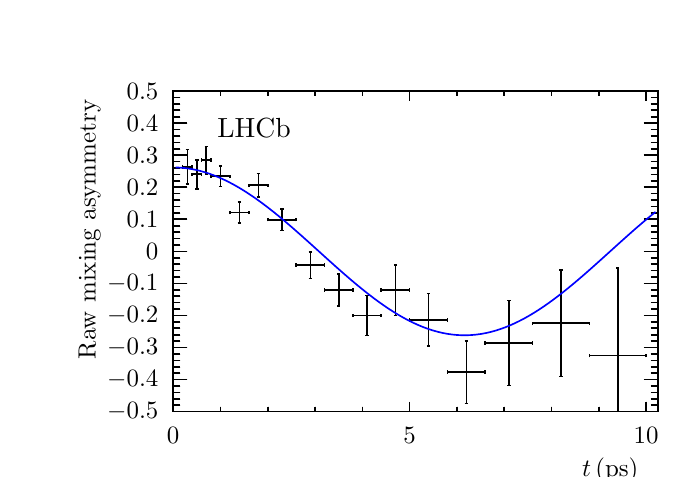
\begin{tikzpicture}[scale=0.38]
\pgfdeclareplotmark{cross} {
\pgfpathmoveto{\pgfpoint{-0.3\pgfplotmarksize}{\pgfplotmarksize}}
\pgfpathlineto{\pgfpoint{+0.3\pgfplotmarksize}{\pgfplotmarksize}}
\pgfpathlineto{\pgfpoint{+0.3\pgfplotmarksize}{0.3\pgfplotmarksize}}
\pgfpathlineto{\pgfpoint{+1\pgfplotmarksize}{0.3\pgfplotmarksize}}
\pgfpathlineto{\pgfpoint{+1\pgfplotmarksize}{-0.3\pgfplotmarksize}}
\pgfpathlineto{\pgfpoint{+0.3\pgfplotmarksize}{-0.3\pgfplotmarksize}}
\pgfpathlineto{\pgfpoint{+0.3\pgfplotmarksize}{-1.\pgfplotmarksize}}
\pgfpathlineto{\pgfpoint{-0.3\pgfplotmarksize}{-1.\pgfplotmarksize}}
\pgfpathlineto{\pgfpoint{-0.3\pgfplotmarksize}{-0.3\pgfplotmarksize}}
\pgfpathlineto{\pgfpoint{-1.\pgfplotmarksize}{-0.3\pgfplotmarksize}}
\pgfpathlineto{\pgfpoint{-1.\pgfplotmarksize}{0.3\pgfplotmarksize}}
\pgfpathlineto{\pgfpoint{-0.3\pgfplotmarksize}{0.3\pgfplotmarksize}}
\pgfpathclose
\pgfusepathqstroke
}
\pgfdeclareplotmark{cross*} {
\pgfpathmoveto{\pgfpoint{-0.3\pgfplotmarksize}{\pgfplotmarksize}}
\pgfpathlineto{\pgfpoint{+0.3\pgfplotmarksize}{\pgfplotmarksize}}
\pgfpathlineto{\pgfpoint{+0.3\pgfplotmarksize}{0.3\pgfplotmarksize}}
\pgfpathlineto{\pgfpoint{+1\pgfplotmarksize}{0.3\pgfplotmarksize}}
\pgfpathlineto{\pgfpoint{+1\pgfplotmarksize}{-0.3\pgfplotmarksize}}
\pgfpathlineto{\pgfpoint{+0.3\pgfplotmarksize}{-0.3\pgfplotmarksize}}
\pgfpathlineto{\pgfpoint{+0.3\pgfplotmarksize}{-1.\pgfplotmarksize}}
\pgfpathlineto{\pgfpoint{-0.3\pgfplotmarksize}{-1.\pgfplotmarksize}}
\pgfpathlineto{\pgfpoint{-0.3\pgfplotmarksize}{-0.3\pgfplotmarksize}}
\pgfpathlineto{\pgfpoint{-1.\pgfplotmarksize}{-0.3\pgfplotmarksize}}
\pgfpathlineto{\pgfpoint{-1.\pgfplotmarksize}{0.3\pgfplotmarksize}}
\pgfpathlineto{\pgfpoint{-0.3\pgfplotmarksize}{0.3\pgfplotmarksize}}
\pgfpathclose
\pgfusepathqfillstroke
}
\pgfdeclareplotmark{newstar} {
\pgfpathmoveto{\pgfqpoint{0pt}{\pgfplotmarksize}}
\pgfpathlineto{\pgfqpointpolar{44}{0.5\pgfplotmarksize}}
\pgfpathlineto{\pgfqpointpolar{18}{\pgfplotmarksize}}
\pgfpathlineto{\pgfqpointpolar{-20}{0.5\pgfplotmarksize}}
\pgfpathlineto{\pgfqpointpolar{-54}{\pgfplotmarksize}}
\pgfpathlineto{\pgfqpointpolar{-90}{0.5\pgfplotmarksize}}
\pgfpathlineto{\pgfqpointpolar{234}{\pgfplotmarksize}}
\pgfpathlineto{\pgfqpointpolar{198}{0.5\pgfplotmarksize}}
\pgfpathlineto{\pgfqpointpolar{162}{\pgfplotmarksize}}
\pgfpathlineto{\pgfqpointpolar{134}{0.5\pgfplotmarksize}}
\pgfpathclose
\pgfusepathqstroke
}
\pgfdeclareplotmark{newstar*} {
\pgfpathmoveto{\pgfqpoint{0pt}{\pgfplotmarksize}}
\pgfpathlineto{\pgfqpointpolar{44}{0.5\pgfplotmarksize}}
\pgfpathlineto{\pgfqpointpolar{18}{\pgfplotmarksize}}
\pgfpathlineto{\pgfqpointpolar{-20}{0.5\pgfplotmarksize}}
\pgfpathlineto{\pgfqpointpolar{-54}{\pgfplotmarksize}}
\pgfpathlineto{\pgfqpointpolar{-90}{0.5\pgfplotmarksize}}
\pgfpathlineto{\pgfqpointpolar{234}{\pgfplotmarksize}}
\pgfpathlineto{\pgfqpointpolar{198}{0.5\pgfplotmarksize}}
\pgfpathlineto{\pgfqpointpolar{162}{\pgfplotmarksize}}
\pgfpathlineto{\pgfqpointpolar{134}{0.5\pgfplotmarksize}}
\pgfpathclose
\pgfusepathqfillstroke
}
\definecolor{c}{rgb}{1,1,1};
\draw [color=c, fill=c] (0,0) rectangle (20,13.5632);
\draw [color=c, fill=c] (2.8,2.17011) rectangle (19,12.8851);
\definecolor{c}{rgb}{0,0,0};
\draw [c,line width=0.6] (2.8,2.17011) -- (2.8,12.8851) -- (19,12.8851) -- (19,2.17011) -- (2.8,2.17011);
\definecolor{c}{rgb}{1,1,1};
\draw [color=c, fill=c] (2.8,2.17011) rectangle (19,12.8851);
\definecolor{c}{rgb}{0,0,0};
\draw [c,line width=0.6] (2.8,2.17011) -- (2.8,12.8851) -- (19,12.8851) -- (19,2.17011) -- (2.8,2.17011);
\draw [c,line width=0.6] (2.8,2.17011) -- (19,2.17011);
\draw [anchor= east] (18.64,0.2) node[scale=0.9, color=c, rotate=0]{$t\,\mathrm{(ps)}$};
\draw [c,line width=0.6] (2.8,2.4997) -- (2.8,2.17011);
\draw [c,line width=0.6] (4.38049,2.33491) -- (4.38049,2.17011);
\draw [c,line width=0.6] (5.96098,2.33491) -- (5.96098,2.17011);
\draw [c,line width=0.6] (7.54146,2.33491) -- (7.54146,2.17011);
\draw [c,line width=0.6] (9.12195,2.33491) -- (9.12195,2.17011);
\draw [c,line width=0.6] (10.7024,2.4997) -- (10.7024,2.17011);
\draw [c,line width=0.6] (12.2829,2.33491) -- (12.2829,2.17011);
\draw [c,line width=0.6] (13.8634,2.33491) -- (13.8634,2.17011);
\draw [c,line width=0.6] (15.4439,2.33491) -- (15.4439,2.17011);
\draw [c,line width=0.6] (17.0244,2.33491) -- (17.0244,2.17011);
\draw [c,line width=0.6] (18.6049,2.4997) -- (18.6049,2.17011);
\draw [c,line width=0.6] (18.6049,2.4997) -- (18.6049,2.17011);
\draw [anchor=base] (2.8,1.1) node[scale=0.9, color=c, rotate=0]{0};
\draw [anchor=base] (10.7024,1.1) node[scale=0.9, color=c, rotate=0]{5};
\draw [anchor=base] (18.6049,1.1) node[scale=0.9, color=c, rotate=0]{10};
\draw [c,line width=0.6] (2.8,12.8851) -- (19,12.8851);
\draw [c,line width=0.6] (2.8,12.5555) -- (2.8,12.8851);
\draw [c,line width=0.6] (4.38049,12.7203) -- (4.38049,12.8851);
\draw [c,line width=0.6] (5.96098,12.7203) -- (5.96098,12.8851);
\draw [c,line width=0.6] (7.54146,12.7203) -- (7.54146,12.8851);
\draw [c,line width=0.6] (9.12195,12.7203) -- (9.12195,12.8851);
\draw [c,line width=0.6] (10.7024,12.5555) -- (10.7024,12.8851);
\draw [c,line width=0.6] (12.2829,12.7203) -- (12.2829,12.8851);
\draw [c,line width=0.6] (13.8634,12.7203) -- (13.8634,12.8851);
\draw [c,line width=0.6] (15.4439,12.7203) -- (15.4439,12.8851);
\draw [c,line width=0.6] (17.0244,12.7203) -- (17.0244,12.8851);
\draw [c,line width=0.6] (18.6049,12.5555) -- (18.6049,12.8851);
\draw [c,line width=0.6] (18.6049,12.5555) -- (18.6049,12.8851);
\draw [c,line width=0.6] (2.8,2.17011) -- (2.8,12.8851);
\draw [anchor= east] (0.,12.8851) node[scale=0.9, color=c, rotate=90]{Raw mixing asymmetry};
\draw [c,line width=0.6] (3.274,2.17011) -- (2.8,2.17011);
\draw [c,line width=0.6] (3.037,2.38441) -- (2.8,2.38441);
\draw [c,line width=0.6] (3.037,2.59871) -- (2.8,2.59871);
\draw [c,line width=0.6] (3.037,2.81301) -- (2.8,2.81301);
\draw [c,line width=0.6] (3.037,3.02731) -- (2.8,3.02731);
\draw [c,line width=0.6] (3.274,3.24161) -- (2.8,3.24161);
\draw [c,line width=0.6] (3.037,3.45591) -- (2.8,3.45591);
\draw [c,line width=0.6] (3.037,3.67021) -- (2.8,3.67021);
\draw [c,line width=0.6] (3.037,3.88451) -- (2.8,3.88451);
\draw [c,line width=0.6] (3.037,4.0988) -- (2.8,4.0988);
\draw [c,line width=0.6] (3.274,4.3131) -- (2.8,4.3131);
\draw [c,line width=0.6] (3.037,4.5274) -- (2.8,4.5274);
\draw [c,line width=0.6] (3.037,4.7417) -- (2.8,4.7417);
\draw [c,line width=0.6] (3.037,4.956) -- (2.8,4.956);
\draw [c,line width=0.6] (3.037,5.1703) -- (2.8,5.1703);
\draw [c,line width=0.6] (3.274,5.3846) -- (2.8,5.3846);
\draw [c,line width=0.6] (3.037,5.5989) -- (2.8,5.5989);
\draw [c,line width=0.6] (3.037,5.8132) -- (2.8,5.8132);
\draw [c,line width=0.6] (3.037,6.02749) -- (2.8,6.02749);
\draw [c,line width=0.6] (3.037,6.24179) -- (2.8,6.24179);
\draw [c,line width=0.6] (3.274,6.45609) -- (2.8,6.45609);
\draw [c,line width=0.6] (3.037,6.67039) -- (2.8,6.67039);
\draw [c,line width=0.6] (3.037,6.88469) -- (2.8,6.88469);
\draw [c,line width=0.6] (3.037,7.09899) -- (2.8,7.09899);
\draw [c,line width=0.6] (3.037,7.31329) -- (2.8,7.31329);
\draw [c,line width=0.6] (3.274,7.52759) -- (2.8,7.52759);
\draw [c,line width=0.6] (3.037,7.74188) -- (2.8,7.74188);
\draw [c,line width=0.6] (3.037,7.95618) -- (2.8,7.95618);
\draw [c,line width=0.6] (3.037,8.17048) -- (2.8,8.17048);
\draw [c,line width=0.6] (3.037,8.38478) -- (2.8,8.38478);
\draw [c,line width=0.6] (3.274,8.59908) -- (2.8,8.59908);
\draw [c,line width=0.6] (3.037,8.81338) -- (2.8,8.81338);
\draw [c,line width=0.6] (3.037,9.02768) -- (2.8,9.02768);
\draw [c,line width=0.6] (3.037,9.24198) -- (2.8,9.24198);
\draw [c,line width=0.6] (3.037,9.45628) -- (2.8,9.45628);
\draw [c,line width=0.6] (3.274,9.67057) -- (2.8,9.67057);
\draw [c,line width=0.6] (3.037,9.88487) -- (2.8,9.88487);
\draw [c,line width=0.6] (3.037,10.0992) -- (2.8,10.0992);
\draw [c,line width=0.6] (3.037,10.3135) -- (2.8,10.3135);
\draw [c,line width=0.6] (3.037,10.5278) -- (2.8,10.5278);
\draw [c,line width=0.6] (3.274,10.7421) -- (2.8,10.7421);
\draw [c,line width=0.6] (3.037,10.9564) -- (2.8,10.9564);
\draw [c,line width=0.6] (3.037,11.1707) -- (2.8,11.1707);
\draw [c,line width=0.6] (3.037,11.385) -- (2.8,11.385);
\draw [c,line width=0.6] (3.037,11.5993) -- (2.8,11.5993);
\draw [c,line width=0.6] (3.274,11.8136) -- (2.8,11.8136);
\draw [c,line width=0.6] (3.037,12.0279) -- (2.8,12.0279);
\draw [c,line width=0.6] (3.037,12.2422) -- (2.8,12.2422);
\draw [c,line width=0.6] (3.037,12.4565) -- (2.8,12.4565);
\draw [c,line width=0.6] (3.037,12.6708) -- (2.8,12.6708);
\draw [c,line width=0.6] (3.274,12.8851) -- (2.8,12.8851);
\draw [c,line width=0.6] (3.274,2.17011) -- (2.8,2.17011);
\draw [anchor= east] (2.6,2.17011) node[scale=0.9, color=c, rotate=0]{$-0.5$};
\draw [anchor= east] (2.6,3.24161) node[scale=0.9, color=c, rotate=0]{$-0.4$};
\draw [anchor= east] (2.6,4.3131) node[scale=0.9, color=c, rotate=0]{$-0.3$};
\draw [anchor= east] (2.6,5.3846) node[scale=0.9, color=c, rotate=0]{$-0.2$};
\draw [anchor= east] (2.6,6.45609) node[scale=0.9, color=c, rotate=0]{$-0.1$};
\draw [anchor= east] (2.6,7.52759) node[scale=0.9, color=c, rotate=0]{$0$};
\draw [anchor= east] (2.6,8.59908) node[scale=0.9, color=c, rotate=0]{$0.1$};
\draw [anchor= east] (2.6,9.67057) node[scale=0.9, color=c, rotate=0]{$0.2$};
\draw [anchor= east] (2.6,10.7421) node[scale=0.9, color=c, rotate=0]{$0.3$};
\draw [anchor= east] (2.6,11.8136) node[scale=0.9, color=c, rotate=0]{$0.4$};
\draw [anchor= east] (2.6,12.8851) node[scale=0.9, color=c, rotate=0]{$0.5$};
\draw [c,line width=0.6] (19,2.17011) -- (19,12.8851);
\draw [c,line width=0.6] (18.526,2.17011) -- (19,2.17011);
\draw [c,line width=0.6] (18.763,2.38441) -- (19,2.38441);
\draw [c,line width=0.6] (18.763,2.59871) -- (19,2.59871);
\draw [c,line width=0.6] (18.763,2.81301) -- (19,2.81301);
\draw [c,line width=0.6] (18.763,3.02731) -- (19,3.02731);
\draw [c,line width=0.6] (18.526,3.24161) -- (19,3.24161);
\draw [c,line width=0.6] (18.763,3.45591) -- (19,3.45591);
\draw [c,line width=0.6] (18.763,3.67021) -- (19,3.67021);
\draw [c,line width=0.6] (18.763,3.88451) -- (19,3.88451);
\draw [c,line width=0.6] (18.763,4.0988) -- (19,4.0988);
\draw [c,line width=0.6] (18.526,4.3131) -- (19,4.3131);
\draw [c,line width=0.6] (18.763,4.5274) -- (19,4.5274);
\draw [c,line width=0.6] (18.763,4.7417) -- (19,4.7417);
\draw [c,line width=0.6] (18.763,4.956) -- (19,4.956);
\draw [c,line width=0.6] (18.763,5.1703) -- (19,5.1703);
\draw [c,line width=0.6] (18.526,5.3846) -- (19,5.3846);
\draw [c,line width=0.6] (18.763,5.5989) -- (19,5.5989);
\draw [c,line width=0.6] (18.763,5.8132) -- (19,5.8132);
\draw [c,line width=0.6] (18.763,6.02749) -- (19,6.02749);
\draw [c,line width=0.6] (18.763,6.24179) -- (19,6.24179);
\draw [c,line width=0.6] (18.526,6.45609) -- (19,6.45609);
\draw [c,line width=0.6] (18.763,6.67039) -- (19,6.67039);
\draw [c,line width=0.6] (18.763,6.88469) -- (19,6.88469);
\draw [c,line width=0.6] (18.763,7.09899) -- (19,7.09899);
\draw [c,line width=0.6] (18.763,7.31329) -- (19,7.31329);
\draw [c,line width=0.6] (18.526,7.52759) -- (19,7.52759);
\draw [c,line width=0.6] (18.763,7.74188) -- (19,7.74188);
\draw [c,line width=0.6] (18.763,7.95618) -- (19,7.95618);
\draw [c,line width=0.6] (18.763,8.17048) -- (19,8.17048);
\draw [c,line width=0.6] (18.763,8.38478) -- (19,8.38478);
\draw [c,line width=0.6] (18.526,8.59908) -- (19,8.59908);
\draw [c,line width=0.6] (18.763,8.81338) -- (19,8.81338);
\draw [c,line width=0.6] (18.763,9.02768) -- (19,9.02768);
\draw [c,line width=0.6] (18.763,9.24198) -- (19,9.24198);
\draw [c,line width=0.6] (18.763,9.45628) -- (19,9.45628);
\draw [c,line width=0.6] (18.526,9.67057) -- (19,9.67057);
\draw [c,line width=0.6] (18.763,9.88487) -- (19,9.88487);
\draw [c,line width=0.6] (18.763,10.0992) -- (19,10.0992);
\draw [c,line width=0.6] (18.763,10.3135) -- (19,10.3135);
\draw [c,line width=0.6] (18.763,10.5278) -- (19,10.5278);
\draw [c,line width=0.6] (18.526,10.7421) -- (19,10.7421);
\draw [c,line width=0.6] (18.763,10.9564) -- (19,10.9564);
\draw [c,line width=0.6] (18.763,11.1707) -- (19,11.1707);
\draw [c,line width=0.6] (18.763,11.385) -- (19,11.385);
\draw [c,line width=0.6] (18.763,11.5993) -- (19,11.5993);
\draw [c,line width=0.6] (18.526,11.8136) -- (19,11.8136);
\draw [c,line width=0.6] (18.763,12.0279) -- (19,12.0279);
\draw [c,line width=0.6] (18.763,12.2422) -- (19,12.2422);
\draw [c,line width=0.6] (18.763,12.4565) -- (19,12.4565);
\draw [c,line width=0.6] (18.763,12.6708) -- (19,12.6708);
\draw [c,line width=0.6] (18.526,12.8851) -- (19,12.8851);
\draw [c,line width=0.6] (18.526,2.17011) -- (19,2.17011);
%\draw [c,line width=0.6] (2.95805,-nan) -- (2.8,-nan);
%\draw [c,line width=0.6] (2.8,-nan) -- (2.8,-nan);
%\draw [c,line width=0.6] (2.95805,-nan) -- (3.1161,-nan);
%\draw [c,line width=0.6] (3.1161,-nan) -- (3.1161,-nan);
\draw [c,line width=0.6] (3.27415,10.3527) -- (3.1161,10.3527);
\draw [c,line width=0.6] (3.1161,10.2953) -- (3.1161,10.4102);
\draw [c,line width=0.6] (3.27415,10.3527) -- (3.4322,10.3527);
\draw [c,line width=0.6] (3.4322,10.2953) -- (3.4322,10.4102);
\draw [c,line width=0.6] (3.27415,10.3527) -- (3.27415,10.9357);
\draw [c,line width=0.6] (3.21668,10.9357) -- (3.33162,10.9357);
\draw [c,line width=0.6] (3.27415,10.3527) -- (3.27415,9.76978);
\draw [c,line width=0.6] (3.21668,9.76978) -- (3.33162,9.76978);
\draw [c,line width=0.6] (3.59024,10.1018) -- (3.4322,10.1018);
\draw [c,line width=0.6] (3.4322,10.0443) -- (3.4322,10.1593);
\draw [c,line width=0.6] (3.59024,10.1018) -- (3.74829,10.1018);
\draw [c,line width=0.6] (3.74829,10.0443) -- (3.74829,10.1593);
\draw [c,line width=0.6] (3.59024,10.1018) -- (3.59024,10.5886);
\draw [c,line width=0.6] (3.53277,10.5886) -- (3.64772,10.5886);
\draw [c,line width=0.6] (3.59024,10.1018) -- (3.59024,9.61499);
\draw [c,line width=0.6] (3.53277,9.61499) -- (3.64772,9.61499);
\draw [c,line width=0.6] (3.90634,10.573) -- (3.74829,10.573);
\draw [c,line width=0.6] (3.74829,10.5155) -- (3.74829,10.6304);
\draw [c,line width=0.6] (3.90634,10.573) -- (4.06439,10.573);
\draw [c,line width=0.6] (4.06439,10.5155) -- (4.06439,10.6304);
\draw [c,line width=0.6] (3.90634,10.573) -- (3.90634,11.0368);
\draw [c,line width=0.6] (3.84887,11.0368) -- (3.96381,11.0368);
\draw [c,line width=0.6] (3.90634,10.573) -- (3.90634,10.1091);
\draw [c,line width=0.6] (3.84887,10.1091) -- (3.96381,10.1091);
\draw [c,line width=0.6] (4.38049,10.0348) -- (4.06439,10.0348);
\draw [c,line width=0.6] (4.06439,9.97734) -- (4.06439,10.0923);
\draw [c,line width=0.6] (4.38049,10.0348) -- (4.69659,10.0348);
\draw [c,line width=0.6] (4.69659,9.97734) -- (4.69659,10.0923);
\draw [c,line width=0.6] (4.38049,10.0348) -- (4.38049,10.373);
\draw [c,line width=0.6] (4.32302,10.373) -- (4.43796,10.373);
\draw [c,line width=0.6] (4.38049,10.0348) -- (4.38049,9.69658);
\draw [c,line width=0.6] (4.32302,9.69658) -- (4.43796,9.69658);
\draw [c,line width=0.6] (5.01268,8.82655) -- (4.69659,8.82655);
\draw [c,line width=0.6] (4.69659,8.76907) -- (4.69659,8.88402);
\draw [c,line width=0.6] (5.01268,8.82655) -- (5.32878,8.82655);
\draw [c,line width=0.6] (5.32878,8.76907) -- (5.32878,8.88402);
\draw [c,line width=0.6] (5.01268,8.82655) -- (5.01268,9.1842);
\draw [c,line width=0.6] (4.95521,9.1842) -- (5.07015,9.1842);
\draw [c,line width=0.6] (5.01268,8.82655) -- (5.01268,8.46889);
\draw [c,line width=0.6] (4.95521,8.46889) -- (5.07015,8.46889);
\draw [c,line width=0.6] (5.64488,9.73599) -- (5.32878,9.73599);
\draw [c,line width=0.6] (5.32878,9.67852) -- (5.32878,9.79346);
\draw [c,line width=0.6] (5.64488,9.73599) -- (5.96098,9.73599);
\draw [c,line width=0.6] (5.96098,9.67852) -- (5.96098,9.79346);
\draw [c,line width=0.6] (5.64488,9.73599) -- (5.64488,10.133);
\draw [c,line width=0.6] (5.58741,10.133) -- (5.70235,10.133);
\draw [c,line width=0.6] (5.64488,9.73599) -- (5.64488,9.33895);
\draw [c,line width=0.6] (5.58741,9.33895) -- (5.70235,9.33895);
\draw [c,line width=0.6] (6.43512,8.58479) -- (5.96098,8.58479);
\draw [c,line width=0.6] (5.96098,8.52732) -- (5.96098,8.64226);
\draw [c,line width=0.6] (6.43512,8.58479) -- (6.90927,8.58479);
\draw [c,line width=0.6] (6.90927,8.52732) -- (6.90927,8.64226);
\draw [c,line width=0.6] (6.43512,8.58479) -- (6.43512,8.94947);
\draw [c,line width=0.6] (6.37765,8.94947) -- (6.49259,8.94947);
\draw [c,line width=0.6] (6.43512,8.58479) -- (6.43512,8.22011);
\draw [c,line width=0.6] (6.37765,8.22011) -- (6.49259,8.22011);
\draw [c,line width=0.6] (7.38341,7.06929) -- (6.90927,7.06929);
\draw [c,line width=0.6] (6.90927,7.01182) -- (6.90927,7.12676);
\draw [c,line width=0.6] (7.38341,7.06929) -- (7.85756,7.06929);
\draw [c,line width=0.6] (7.85756,7.01182) -- (7.85756,7.12676);
\draw [c,line width=0.6] (7.38341,7.06929) -- (7.38341,7.51456);
\draw [c,line width=0.6] (7.32594,7.51456) -- (7.44089,7.51456);
\draw [c,line width=0.6] (7.38341,7.06929) -- (7.38341,6.62402);
\draw [c,line width=0.6] (7.32594,6.62402) -- (7.44089,6.62402);
\draw [c,line width=0.6] (8.33171,6.23438) -- (7.85756,6.23438);
\draw [c,line width=0.6] (7.85756,6.17691) -- (7.85756,6.29185);
\draw [c,line width=0.6] (8.33171,6.23438) -- (8.80585,6.23438);
\draw [c,line width=0.6] (8.80585,6.17691) -- (8.80585,6.29185);
\draw [c,line width=0.6] (8.33171,6.23438) -- (8.33171,6.76703);
\draw [c,line width=0.6] (8.27424,6.76703) -- (8.38918,6.76703);
\draw [c,line width=0.6] (8.33171,6.23438) -- (8.33171,5.70173);
\draw [c,line width=0.6] (8.27424,5.70173) -- (8.38918,5.70173);
\draw [c,line width=0.6] (9.28,5.38618) -- (8.80585,5.38618);
\draw [c,line width=0.6] (8.80585,5.3287) -- (8.80585,5.44365);
\draw [c,line width=0.6] (9.28,5.38618) -- (9.75415,5.38618);
\draw [c,line width=0.6] (9.75415,5.3287) -- (9.75415,5.44365);
\draw [c,line width=0.6] (9.28,5.38618) -- (9.28,6.05488);
\draw [c,line width=0.6] (9.22253,6.05488) -- (9.33747,6.05488);
\draw [c,line width=0.6] (9.28,5.38618) -- (9.28,4.71748);
\draw [c,line width=0.6] (9.22253,4.71748) -- (9.33747,4.71748);
\draw [c,line width=0.6] (10.2283,6.22956) -- (9.75415,6.22956);
\draw [c,line width=0.6] (9.75415,6.17209) -- (9.75415,6.28703);
\draw [c,line width=0.6] (10.2283,6.22956) -- (10.7024,6.22956);
\draw [c,line width=0.6] (10.7024,6.17209) -- (10.7024,6.28703);
\draw [c,line width=0.6] (10.2283,6.22956) -- (10.2283,7.07638);
\draw [c,line width=0.6] (10.1708,7.07638) -- (10.2858,7.07638);
\draw [c,line width=0.6] (10.2283,6.22956) -- (10.2283,5.38274);
\draw [c,line width=0.6] (10.1708,5.38274) -- (10.2858,5.38274);
\draw [c,line width=0.6] (11.3346,5.23405) -- (10.7024,5.23405);
\draw [c,line width=0.6] (10.7024,5.17658) -- (10.7024,5.29152);
\draw [c,line width=0.6] (11.3346,5.23405) -- (11.9668,5.23405);
\draw [c,line width=0.6] (11.9668,5.17658) -- (11.9668,5.29152);
\draw [c,line width=0.6] (11.3346,5.23405) -- (11.3346,6.11496);
\draw [c,line width=0.6] (11.2772,6.11496) -- (11.3921,6.11496);
\draw [c,line width=0.6] (11.3346,5.23405) -- (11.3346,4.35313);
\draw [c,line width=0.6] (11.2772,4.35313) -- (11.3921,4.35313);
\draw [c,line width=0.6] (12.599,3.48937) -- (11.9668,3.48937);
\draw [c,line width=0.6] (11.9668,3.4319) -- (11.9668,3.54685);
\draw [c,line width=0.6] (12.599,3.48937) -- (13.2312,3.48937);
\draw [c,line width=0.6] (13.2312,3.4319) -- (13.2312,3.54685);
\draw [c,line width=0.6] (12.599,3.48937) -- (12.599,4.5374);
\draw [c,line width=0.6] (12.5416,4.5374) -- (12.6565,4.5374);
\draw [c,line width=0.6] (12.599,3.48937) -- (12.599,2.44135);
\draw [c,line width=0.6] (12.5416,2.44135) -- (12.6565,2.44135);
\draw [c,line width=0.6] (14.0215,4.46426) -- (13.2312,4.46426);
\draw [c,line width=0.6] (13.2312,4.40679) -- (13.2312,4.52173);
\draw [c,line width=0.6] (14.0215,4.46426) -- (14.8117,4.46426);
\draw [c,line width=0.6] (14.8117,4.40679) -- (14.8117,4.52173);
\draw [c,line width=0.6] (14.0215,4.46426) -- (14.0215,5.88686);
\draw [c,line width=0.6] (13.964,5.88686) -- (14.0789,5.88686);
\draw [c,line width=0.6] (14.0215,4.46426) -- (14.0215,3.04165);
\draw [c,line width=0.6] (13.964,3.04165) -- (14.0789,3.04165);
\draw [c,line width=0.6] (15.76,5.12313) -- (14.8117,5.12313);
\draw [c,line width=0.6] (14.8117,5.06566) -- (14.8117,5.18061);
\draw [c,line width=0.6] (15.76,5.12313) -- (16.7083,5.12313);
\draw [c,line width=0.6] (16.7083,5.06566) -- (16.7083,5.18061);
\draw [c,line width=0.6] (15.76,5.12313) -- (15.76,6.90155);
\draw [c,line width=0.6] (15.7025,6.90155) -- (15.8175,6.90155);
\draw [c,line width=0.6] (15.76,5.12313) -- (15.76,3.34472);
\draw [c,line width=0.6] (15.7025,3.34472) -- (15.8175,3.34472);
\draw [c,line width=0.6] (17.6566,4.04359) -- (16.7083,4.04359);
\draw [c,line width=0.6] (16.7083,3.98611) -- (16.7083,4.10106);
\draw [c,line width=0.6] (17.6566,4.04359) -- (18.6049,4.04359);
\draw [c,line width=0.6] (18.6049,3.98611) -- (18.6049,4.10106);
\draw [c,line width=0.6] (17.6566,4.04359) -- (17.6566,6.98076);
\draw [c,line width=0.6] (17.5991,6.98076) -- (17.7141,6.98076);
\draw [c,line width=0.6] (17.6566,4.04359) -- (17.6566,2.17011);
\draw [c,line width=0.6] (17.5991,2.17011) -- (17.7141,2.17011);
\foreach \P in
 {(3.27415,10.3527),(3.59024,10.1018),(3.90634,10.573),(4.38049,10.0348),(5.01268,8.82655),(5.64488,9.73599),(6.43512,8.58479),(7.38341,7.06929),(8.33171,6.23438),(9.28,5.38618),(10.2283,6.22956),(11.3346,5.23405),(12.599,3.48937),(14.0215,4.46426),(
15.76,5.12313),(17.6566,4.04359)}{\draw[mark options={color=c,fill=c},mark size=2.402402pt,mark=] plot coordinates {\P};}
\draw [c,line width=0.6] (2.8,2.17011) -- (19,2.17011);
\draw [c,line width=0.6] (2.8,2.4997) -- (2.8,2.17011);
\draw [c,line width=0.6] (4.38049,2.33491) -- (4.38049,2.17011);
\draw [c,line width=0.6] (5.96098,2.33491) -- (5.96098,2.17011);
\draw [c,line width=0.6] (7.54146,2.33491) -- (7.54146,2.17011);
\draw [c,line width=0.6] (9.12195,2.33491) -- (9.12195,2.17011);
\draw [c,line width=0.6] (10.7024,2.4997) -- (10.7024,2.17011);
\draw [c,line width=0.6] (12.2829,2.33491) -- (12.2829,2.17011);
\draw [c,line width=0.6] (13.8634,2.33491) -- (13.8634,2.17011);
\draw [c,line width=0.6] (15.4439,2.33491) -- (15.4439,2.17011);
\draw [c,line width=0.6] (17.0244,2.33491) -- (17.0244,2.17011);
\draw [c,line width=0.6] (18.6049,2.4997) -- (18.6049,2.17011);
\draw [c,line width=0.6] (18.6049,2.4997) -- (18.6049,2.17011);
\draw [c,line width=0.6] (2.8,12.8851) -- (19,12.8851);
\draw [c,line width=0.6] (2.8,12.5555) -- (2.8,12.8851);
\draw [c,line width=0.6] (4.38049,12.7203) -- (4.38049,12.8851);
\draw [c,line width=0.6] (5.96098,12.7203) -- (5.96098,12.8851);
\draw [c,line width=0.6] (7.54146,12.7203) -- (7.54146,12.8851);
\draw [c,line width=0.6] (9.12195,12.7203) -- (9.12195,12.8851);
\draw [c,line width=0.6] (10.7024,12.5555) -- (10.7024,12.8851);
\draw [c,line width=0.6] (12.2829,12.7203) -- (12.2829,12.8851);
\draw [c,line width=0.6] (13.8634,12.7203) -- (13.8634,12.8851);
\draw [c,line width=0.6] (15.4439,12.7203) -- (15.4439,12.8851);
\draw [c,line width=0.6] (17.0244,12.7203) -- (17.0244,12.8851);
\draw [c,line width=0.6] (18.6049,12.5555) -- (18.6049,12.8851);
\draw [c,line width=0.6] (18.6049,12.5555) -- (18.6049,12.8851);
\draw [c,line width=0.6] (2.8,2.17011) -- (2.8,12.8851);
\draw [c,line width=0.6] (3.274,2.17011) -- (2.8,2.17011);
\draw [c,line width=0.6] (3.037,2.38441) -- (2.8,2.38441);
\draw [c,line width=0.6] (3.037,2.59871) -- (2.8,2.59871);
\draw [c,line width=0.6] (3.037,2.81301) -- (2.8,2.81301);
\draw [c,line width=0.6] (3.037,3.02731) -- (2.8,3.02731);
\draw [c,line width=0.6] (3.274,3.24161) -- (2.8,3.24161);
\draw [c,line width=0.6] (3.037,3.45591) -- (2.8,3.45591);
\draw [c,line width=0.6] (3.037,3.67021) -- (2.8,3.67021);
\draw [c,line width=0.6] (3.037,3.88451) -- (2.8,3.88451);
\draw [c,line width=0.6] (3.037,4.0988) -- (2.8,4.0988);
\draw [c,line width=0.6] (3.274,4.3131) -- (2.8,4.3131);
\draw [c,line width=0.6] (3.037,4.5274) -- (2.8,4.5274);
\draw [c,line width=0.6] (3.037,4.7417) -- (2.8,4.7417);
\draw [c,line width=0.6] (3.037,4.956) -- (2.8,4.956);
\draw [c,line width=0.6] (3.037,5.1703) -- (2.8,5.1703);
\draw [c,line width=0.6] (3.274,5.3846) -- (2.8,5.3846);
\draw [c,line width=0.6] (3.037,5.5989) -- (2.8,5.5989);
\draw [c,line width=0.6] (3.037,5.8132) -- (2.8,5.8132);
\draw [c,line width=0.6] (3.037,6.02749) -- (2.8,6.02749);
\draw [c,line width=0.6] (3.037,6.24179) -- (2.8,6.24179);
\draw [c,line width=0.6] (3.274,6.45609) -- (2.8,6.45609);
\draw [c,line width=0.6] (3.037,6.67039) -- (2.8,6.67039);
\draw [c,line width=0.6] (3.037,6.88469) -- (2.8,6.88469);
\draw [c,line width=0.6] (3.037,7.09899) -- (2.8,7.09899);
\draw [c,line width=0.6] (3.037,7.31329) -- (2.8,7.31329);
\draw [c,line width=0.6] (3.274,7.52759) -- (2.8,7.52759);
\draw [c,line width=0.6] (3.037,7.74188) -- (2.8,7.74188);
\draw [c,line width=0.6] (3.037,7.95618) -- (2.8,7.95618);
\draw [c,line width=0.6] (3.037,8.17048) -- (2.8,8.17048);
\draw [c,line width=0.6] (3.037,8.38478) -- (2.8,8.38478);
\draw [c,line width=0.6] (3.274,8.59908) -- (2.8,8.59908);
\draw [c,line width=0.6] (3.037,8.81338) -- (2.8,8.81338);
\draw [c,line width=0.6] (3.037,9.02768) -- (2.8,9.02768);
\draw [c,line width=0.6] (3.037,9.24198) -- (2.8,9.24198);
\draw [c,line width=0.6] (3.037,9.45628) -- (2.8,9.45628);
\draw [c,line width=0.6] (3.274,9.67057) -- (2.8,9.67057);
\draw [c,line width=0.6] (3.037,9.88487) -- (2.8,9.88487);
\draw [c,line width=0.6] (3.037,10.0992) -- (2.8,10.0992);
\draw [c,line width=0.6] (3.037,10.3135) -- (2.8,10.3135);
\draw [c,line width=0.6] (3.037,10.5278) -- (2.8,10.5278);
\draw [c,line width=0.6] (3.274,10.7421) -- (2.8,10.7421);
\draw [c,line width=0.6] (3.037,10.9564) -- (2.8,10.9564);
\draw [c,line width=0.6] (3.037,11.1707) -- (2.8,11.1707);
\draw [c,line width=0.6] (3.037,11.385) -- (2.8,11.385);
\draw [c,line width=0.6] (3.037,11.5993) -- (2.8,11.5993);
\draw [c,line width=0.6] (3.274,11.8136) -- (2.8,11.8136);
\draw [c,line width=0.6] (3.037,12.0279) -- (2.8,12.0279);
\draw [c,line width=0.6] (3.037,12.2422) -- (2.8,12.2422);
\draw [c,line width=0.6] (3.037,12.4565) -- (2.8,12.4565);
\draw [c,line width=0.6] (3.037,12.6708) -- (2.8,12.6708);
\draw [c,line width=0.6] (3.274,12.8851) -- (2.8,12.8851);
\draw [c,line width=0.6] (3.274,2.17011) -- (2.8,2.17011);
\draw [c,line width=0.6] (19,2.17011) -- (19,12.8851);
\draw [c,line width=0.6] (18.526,2.17011) -- (19,2.17011);
\draw [c,line width=0.6] (18.763,2.38441) -- (19,2.38441);
\draw [c,line width=0.6] (18.763,2.59871) -- (19,2.59871);
\draw [c,line width=0.6] (18.763,2.81301) -- (19,2.81301);
\draw [c,line width=0.6] (18.763,3.02731) -- (19,3.02731);
\draw [c,line width=0.6] (18.526,3.24161) -- (19,3.24161);
\draw [c,line width=0.6] (18.763,3.45591) -- (19,3.45591);
\draw [c,line width=0.6] (18.763,3.67021) -- (19,3.67021);
\draw [c,line width=0.6] (18.763,3.88451) -- (19,3.88451);
\draw [c,line width=0.6] (18.763,4.0988) -- (19,4.0988);
\draw [c,line width=0.6] (18.526,4.3131) -- (19,4.3131);
\draw [c,line width=0.6] (18.763,4.5274) -- (19,4.5274);
\draw [c,line width=0.6] (18.763,4.7417) -- (19,4.7417);
\draw [c,line width=0.6] (18.763,4.956) -- (19,4.956);
\draw [c,line width=0.6] (18.763,5.1703) -- (19,5.1703);
\draw [c,line width=0.6] (18.526,5.3846) -- (19,5.3846);
\draw [c,line width=0.6] (18.763,5.5989) -- (19,5.5989);
\draw [c,line width=0.6] (18.763,5.8132) -- (19,5.8132);
\draw [c,line width=0.6] (18.763,6.02749) -- (19,6.02749);
\draw [c,line width=0.6] (18.763,6.24179) -- (19,6.24179);
\draw [c,line width=0.6] (18.526,6.45609) -- (19,6.45609);
\draw [c,line width=0.6] (18.763,6.67039) -- (19,6.67039);
\draw [c,line width=0.6] (18.763,6.88469) -- (19,6.88469);
\draw [c,line width=0.6] (18.763,7.09899) -- (19,7.09899);
\draw [c,line width=0.6] (18.763,7.31329) -- (19,7.31329);
\draw [c,line width=0.6] (18.526,7.52759) -- (19,7.52759);
\draw [c,line width=0.6] (18.763,7.74188) -- (19,7.74188);
\draw [c,line width=0.6] (18.763,7.95618) -- (19,7.95618);
\draw [c,line width=0.6] (18.763,8.17048) -- (19,8.17048);
\draw [c,line width=0.6] (18.763,8.38478) -- (19,8.38478);
\draw [c,line width=0.6] (18.526,8.59908) -- (19,8.59908);
\draw [c,line width=0.6] (18.763,8.81338) -- (19,8.81338);
\draw [c,line width=0.6] (18.763,9.02768) -- (19,9.02768);
\draw [c,line width=0.6] (18.763,9.24198) -- (19,9.24198);
\draw [c,line width=0.6] (18.763,9.45628) -- (19,9.45628);
\draw [c,line width=0.6] (18.526,9.67057) -- (19,9.67057);
\draw [c,line width=0.6] (18.763,9.88487) -- (19,9.88487);
\draw [c,line width=0.6] (18.763,10.0992) -- (19,10.0992);
\draw [c,line width=0.6] (18.763,10.3135) -- (19,10.3135);
\draw [c,line width=0.6] (18.763,10.5278) -- (19,10.5278);
\draw [c,line width=0.6] (18.526,10.7421) -- (19,10.7421);
\draw [c,line width=0.6] (18.763,10.9564) -- (19,10.9564);
\draw [c,line width=0.6] (18.763,11.1707) -- (19,11.1707);
\draw [c,line width=0.6] (18.763,11.385) -- (19,11.385);
\draw [c,line width=0.6] (18.763,11.5993) -- (19,11.5993);
\draw [c,line width=0.6] (18.526,11.8136) -- (19,11.8136);
\draw [c,line width=0.6] (18.763,12.0279) -- (19,12.0279);
\draw [c,line width=0.6] (18.763,12.2422) -- (19,12.2422);
\draw [c,line width=0.6] (18.763,12.4565) -- (19,12.4565);
\draw [c,line width=0.6] (18.763,12.6708) -- (19,12.6708);
\draw [c,line width=0.6] (18.526,12.8851) -- (19,12.8851);
\draw [c,line width=0.6] (18.526,2.17011) -- (19,2.17011);
\definecolor{c}{rgb}{0,0,1};
\draw [c,line width=0.6] (2.881,10.3318) -- (3.043,10.3242) -- (3.205,10.3089) -- (3.367,10.286) -- (3.529,10.2555) -- (3.691,10.2176) -- (3.853,10.1724) -- (4.015,10.1199) -- (4.177,10.0604) -- (4.339,9.99392) -- (4.501,9.92071) -- (4.663,9.84097)
 -- (4.825,9.75491) -- (4.987,9.66276) -- (5.149,9.56478) -- (5.311,9.46123) -- (5.473,9.3524) -- (5.635,9.23858) -- (5.797,9.12009) -- (5.959,8.99725) -- (6.121,8.8704) -- (6.283,8.73987) -- (6.445,8.60603) -- (6.607,8.46925) -- (6.769,8.3299) --
 (6.931,8.18835) -- (7.093,8.04499) -- (7.255,7.90023) -- (7.417,7.75444) -- (7.579,7.60804) -- (7.741,7.46141) -- (7.903,7.31497) -- (8.065,7.16911) -- (8.227,7.02422) -- (8.389,6.88072) -- (8.551,6.73898) -- (8.713,6.59939) -- (8.875,6.46234) --
 (9.037,6.3282) -- (9.199,6.19734) -- (9.361,6.07011) -- (9.523,5.94686) -- (9.685,5.82793) -- (9.847,5.71365) -- (10.009,5.60432) -- (10.171,5.50024) -- (10.333,5.40171) -- (10.495,5.30898) -- (10.657,5.22231) -- (10.819,5.14194);
\draw [c,line width=0.6] (10.819,5.14194) -- (10.981,5.06809) -- (11.143,5.00096) -- (11.305,4.94073) -- (11.467,4.88757) -- (11.629,4.84163) -- (11.791,4.80302) -- (11.953,4.77185) -- (12.115,4.74821) -- (12.277,4.73217) -- (12.439,4.72376) --
 (12.601,4.72301) -- (12.763,4.72993) -- (12.925,4.74449) -- (13.087,4.76665) -- (13.249,4.79636) -- (13.411,4.83352) -- (13.573,4.87805) -- (13.735,4.92982) -- (13.897,4.98868) -- (14.059,5.05448) -- (14.221,5.12704) -- (14.383,5.20615) --
 (14.545,5.29161) -- (14.707,5.38318) -- (14.869,5.4806) -- (15.031,5.58362) -- (15.193,5.69195) -- (15.355,5.80529) -- (15.517,5.92334) -- (15.679,6.04577) -- (15.841,6.17225) -- (16.003,6.30243) -- (16.165,6.43596) -- (16.327,6.57248) --
 (16.489,6.7116) -- (16.651,6.85295) -- (16.813,6.99614) -- (16.975,7.14079) -- (17.137,7.28649) -- (17.299,7.43285) -- (17.461,7.57947) -- (17.623,7.72595) -- (17.785,7.87189) -- (17.947,8.01689) -- (18.109,8.16055) -- (18.271,8.30248) --
 (18.433,8.44229) -- (18.595,8.5796) -- (18.757,8.71404);
\draw [c,line width=0.6] (18.757,8.71404) -- (18.919,8.84524);
\definecolor{c}{rgb}{1,1,1};
\draw [color=c, fill=c] (3.8,11.1218) rectangle (6.8,12.2069);
\definecolor{c}{rgb}{0,0,0};
\draw [anchor= west] (3.95,11.6644) node[scale=1, color=c, rotate=0]{LHCb};

\end{tikzpicture}
\endpgfgraphicnamed

\beginpgfgraphicnamed{pdf/DsD_MixingAsym_SSComb}
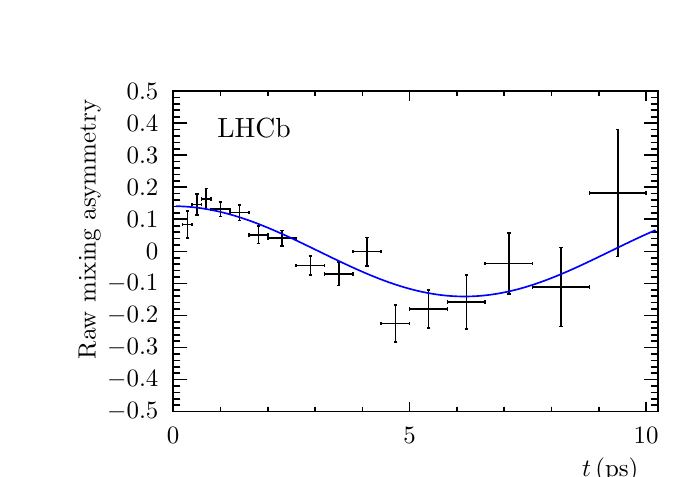
\begin{tikzpicture}[scale=0.38]
\pgfdeclareplotmark{cross} {
\pgfpathmoveto{\pgfpoint{-0.3\pgfplotmarksize}{\pgfplotmarksize}}
\pgfpathlineto{\pgfpoint{+0.3\pgfplotmarksize}{\pgfplotmarksize}}
\pgfpathlineto{\pgfpoint{+0.3\pgfplotmarksize}{0.3\pgfplotmarksize}}
\pgfpathlineto{\pgfpoint{+1\pgfplotmarksize}{0.3\pgfplotmarksize}}
\pgfpathlineto{\pgfpoint{+1\pgfplotmarksize}{-0.3\pgfplotmarksize}}
\pgfpathlineto{\pgfpoint{+0.3\pgfplotmarksize}{-0.3\pgfplotmarksize}}
\pgfpathlineto{\pgfpoint{+0.3\pgfplotmarksize}{-1.\pgfplotmarksize}}
\pgfpathlineto{\pgfpoint{-0.3\pgfplotmarksize}{-1.\pgfplotmarksize}}
\pgfpathlineto{\pgfpoint{-0.3\pgfplotmarksize}{-0.3\pgfplotmarksize}}
\pgfpathlineto{\pgfpoint{-1.\pgfplotmarksize}{-0.3\pgfplotmarksize}}
\pgfpathlineto{\pgfpoint{-1.\pgfplotmarksize}{0.3\pgfplotmarksize}}
\pgfpathlineto{\pgfpoint{-0.3\pgfplotmarksize}{0.3\pgfplotmarksize}}
\pgfpathclose
\pgfusepathqstroke
}
\pgfdeclareplotmark{cross*} {
\pgfpathmoveto{\pgfpoint{-0.3\pgfplotmarksize}{\pgfplotmarksize}}
\pgfpathlineto{\pgfpoint{+0.3\pgfplotmarksize}{\pgfplotmarksize}}
\pgfpathlineto{\pgfpoint{+0.3\pgfplotmarksize}{0.3\pgfplotmarksize}}
\pgfpathlineto{\pgfpoint{+1\pgfplotmarksize}{0.3\pgfplotmarksize}}
\pgfpathlineto{\pgfpoint{+1\pgfplotmarksize}{-0.3\pgfplotmarksize}}
\pgfpathlineto{\pgfpoint{+0.3\pgfplotmarksize}{-0.3\pgfplotmarksize}}
\pgfpathlineto{\pgfpoint{+0.3\pgfplotmarksize}{-1.\pgfplotmarksize}}
\pgfpathlineto{\pgfpoint{-0.3\pgfplotmarksize}{-1.\pgfplotmarksize}}
\pgfpathlineto{\pgfpoint{-0.3\pgfplotmarksize}{-0.3\pgfplotmarksize}}
\pgfpathlineto{\pgfpoint{-1.\pgfplotmarksize}{-0.3\pgfplotmarksize}}
\pgfpathlineto{\pgfpoint{-1.\pgfplotmarksize}{0.3\pgfplotmarksize}}
\pgfpathlineto{\pgfpoint{-0.3\pgfplotmarksize}{0.3\pgfplotmarksize}}
\pgfpathclose
\pgfusepathqfillstroke
}
\pgfdeclareplotmark{newstar} {
\pgfpathmoveto{\pgfqpoint{0pt}{\pgfplotmarksize}}
\pgfpathlineto{\pgfqpointpolar{44}{0.5\pgfplotmarksize}}
\pgfpathlineto{\pgfqpointpolar{18}{\pgfplotmarksize}}
\pgfpathlineto{\pgfqpointpolar{-20}{0.5\pgfplotmarksize}}
\pgfpathlineto{\pgfqpointpolar{-54}{\pgfplotmarksize}}
\pgfpathlineto{\pgfqpointpolar{-90}{0.5\pgfplotmarksize}}
\pgfpathlineto{\pgfqpointpolar{234}{\pgfplotmarksize}}
\pgfpathlineto{\pgfqpointpolar{198}{0.5\pgfplotmarksize}}
\pgfpathlineto{\pgfqpointpolar{162}{\pgfplotmarksize}}
\pgfpathlineto{\pgfqpointpolar{134}{0.5\pgfplotmarksize}}
\pgfpathclose
\pgfusepathqstroke
}
\pgfdeclareplotmark{newstar*} {
\pgfpathmoveto{\pgfqpoint{0pt}{\pgfplotmarksize}}
\pgfpathlineto{\pgfqpointpolar{44}{0.5\pgfplotmarksize}}
\pgfpathlineto{\pgfqpointpolar{18}{\pgfplotmarksize}}
\pgfpathlineto{\pgfqpointpolar{-20}{0.5\pgfplotmarksize}}
\pgfpathlineto{\pgfqpointpolar{-54}{\pgfplotmarksize}}
\pgfpathlineto{\pgfqpointpolar{-90}{0.5\pgfplotmarksize}}
\pgfpathlineto{\pgfqpointpolar{234}{\pgfplotmarksize}}
\pgfpathlineto{\pgfqpointpolar{198}{0.5\pgfplotmarksize}}
\pgfpathlineto{\pgfqpointpolar{162}{\pgfplotmarksize}}
\pgfpathlineto{\pgfqpointpolar{134}{0.5\pgfplotmarksize}}
\pgfpathclose
\pgfusepathqfillstroke
}
\definecolor{c}{rgb}{1,1,1};
\draw [color=c, fill=c] (0,0) rectangle (20,13.5632);
\draw [color=c, fill=c] (2.8,2.17011) rectangle (19,12.8851);
\definecolor{c}{rgb}{0,0,0};
\draw [c,line width=0.6] (2.8,2.17011) -- (2.8,12.8851) -- (19,12.8851) -- (19,2.17011) -- (2.8,2.17011);
\definecolor{c}{rgb}{1,1,1};
\draw [color=c, fill=c] (2.8,2.17011) rectangle (19,12.8851);
\definecolor{c}{rgb}{0,0,0};
\draw [c,line width=0.6] (2.8,2.17011) -- (2.8,12.8851) -- (19,12.8851) -- (19,2.17011) -- (2.8,2.17011);
\draw [c,line width=0.6] (2.8,2.17011) -- (19,2.17011);
\draw [anchor= east] (18.64,0.2) node[scale=0.9, color=c, rotate=0]{$t\,\mathrm{(ps)}$};
\draw [c,line width=0.6] (2.8,2.4997) -- (2.8,2.17011);
\draw [c,line width=0.6] (4.38049,2.33491) -- (4.38049,2.17011);
\draw [c,line width=0.6] (5.96098,2.33491) -- (5.96098,2.17011);
\draw [c,line width=0.6] (7.54146,2.33491) -- (7.54146,2.17011);
\draw [c,line width=0.6] (9.12195,2.33491) -- (9.12195,2.17011);
\draw [c,line width=0.6] (10.7024,2.4997) -- (10.7024,2.17011);
\draw [c,line width=0.6] (12.2829,2.33491) -- (12.2829,2.17011);
\draw [c,line width=0.6] (13.8634,2.33491) -- (13.8634,2.17011);
\draw [c,line width=0.6] (15.4439,2.33491) -- (15.4439,2.17011);
\draw [c,line width=0.6] (17.0244,2.33491) -- (17.0244,2.17011);
\draw [c,line width=0.6] (18.6049,2.4997) -- (18.6049,2.17011);
\draw [c,line width=0.6] (18.6049,2.4997) -- (18.6049,2.17011);
\draw [anchor=base] (2.8,1.1) node[scale=0.9, color=c, rotate=0]{0};
\draw [anchor=base] (10.7024,1.1) node[scale=0.9, color=c, rotate=0]{5};
\draw [anchor=base] (18.6049,1.1) node[scale=0.9, color=c, rotate=0]{10};
\draw [c,line width=0.6] (2.8,12.8851) -- (19,12.8851);
\draw [c,line width=0.6] (2.8,12.5555) -- (2.8,12.8851);
\draw [c,line width=0.6] (4.38049,12.7203) -- (4.38049,12.8851);
\draw [c,line width=0.6] (5.96098,12.7203) -- (5.96098,12.8851);
\draw [c,line width=0.6] (7.54146,12.7203) -- (7.54146,12.8851);
\draw [c,line width=0.6] (9.12195,12.7203) -- (9.12195,12.8851);
\draw [c,line width=0.6] (10.7024,12.5555) -- (10.7024,12.8851);
\draw [c,line width=0.6] (12.2829,12.7203) -- (12.2829,12.8851);
\draw [c,line width=0.6] (13.8634,12.7203) -- (13.8634,12.8851);
\draw [c,line width=0.6] (15.4439,12.7203) -- (15.4439,12.8851);
\draw [c,line width=0.6] (17.0244,12.7203) -- (17.0244,12.8851);
\draw [c,line width=0.6] (18.6049,12.5555) -- (18.6049,12.8851);
\draw [c,line width=0.6] (18.6049,12.5555) -- (18.6049,12.8851);
\draw [c,line width=0.6] (2.8,2.17011) -- (2.8,12.8851);
\draw [anchor= east] (0.,12.8851) node[scale=0.9, color=c, rotate=90]{Raw mixing asymmetry};
\draw [c,line width=0.6] (3.274,2.17011) -- (2.8,2.17011);
\draw [c,line width=0.6] (3.037,2.38441) -- (2.8,2.38441);
\draw [c,line width=0.6] (3.037,2.59871) -- (2.8,2.59871);
\draw [c,line width=0.6] (3.037,2.81301) -- (2.8,2.81301);
\draw [c,line width=0.6] (3.037,3.02731) -- (2.8,3.02731);
\draw [c,line width=0.6] (3.274,3.24161) -- (2.8,3.24161);
\draw [c,line width=0.6] (3.037,3.45591) -- (2.8,3.45591);
\draw [c,line width=0.6] (3.037,3.67021) -- (2.8,3.67021);
\draw [c,line width=0.6] (3.037,3.88451) -- (2.8,3.88451);
\draw [c,line width=0.6] (3.037,4.0988) -- (2.8,4.0988);
\draw [c,line width=0.6] (3.274,4.3131) -- (2.8,4.3131);
\draw [c,line width=0.6] (3.037,4.5274) -- (2.8,4.5274);
\draw [c,line width=0.6] (3.037,4.7417) -- (2.8,4.7417);
\draw [c,line width=0.6] (3.037,4.956) -- (2.8,4.956);
\draw [c,line width=0.6] (3.037,5.1703) -- (2.8,5.1703);
\draw [c,line width=0.6] (3.274,5.3846) -- (2.8,5.3846);
\draw [c,line width=0.6] (3.037,5.5989) -- (2.8,5.5989);
\draw [c,line width=0.6] (3.037,5.8132) -- (2.8,5.8132);
\draw [c,line width=0.6] (3.037,6.02749) -- (2.8,6.02749);
\draw [c,line width=0.6] (3.037,6.24179) -- (2.8,6.24179);
\draw [c,line width=0.6] (3.274,6.45609) -- (2.8,6.45609);
\draw [c,line width=0.6] (3.037,6.67039) -- (2.8,6.67039);
\draw [c,line width=0.6] (3.037,6.88469) -- (2.8,6.88469);
\draw [c,line width=0.6] (3.037,7.09899) -- (2.8,7.09899);
\draw [c,line width=0.6] (3.037,7.31329) -- (2.8,7.31329);
\draw [c,line width=0.6] (3.274,7.52759) -- (2.8,7.52759);
\draw [c,line width=0.6] (3.037,7.74188) -- (2.8,7.74188);
\draw [c,line width=0.6] (3.037,7.95618) -- (2.8,7.95618);
\draw [c,line width=0.6] (3.037,8.17048) -- (2.8,8.17048);
\draw [c,line width=0.6] (3.037,8.38478) -- (2.8,8.38478);
\draw [c,line width=0.6] (3.274,8.59908) -- (2.8,8.59908);
\draw [c,line width=0.6] (3.037,8.81338) -- (2.8,8.81338);
\draw [c,line width=0.6] (3.037,9.02768) -- (2.8,9.02768);
\draw [c,line width=0.6] (3.037,9.24198) -- (2.8,9.24198);
\draw [c,line width=0.6] (3.037,9.45628) -- (2.8,9.45628);
\draw [c,line width=0.6] (3.274,9.67057) -- (2.8,9.67057);
\draw [c,line width=0.6] (3.037,9.88487) -- (2.8,9.88487);
\draw [c,line width=0.6] (3.037,10.0992) -- (2.8,10.0992);
\draw [c,line width=0.6] (3.037,10.3135) -- (2.8,10.3135);
\draw [c,line width=0.6] (3.037,10.5278) -- (2.8,10.5278);
\draw [c,line width=0.6] (3.274,10.7421) -- (2.8,10.7421);
\draw [c,line width=0.6] (3.037,10.9564) -- (2.8,10.9564);
\draw [c,line width=0.6] (3.037,11.1707) -- (2.8,11.1707);
\draw [c,line width=0.6] (3.037,11.385) -- (2.8,11.385);
\draw [c,line width=0.6] (3.037,11.5993) -- (2.8,11.5993);
\draw [c,line width=0.6] (3.274,11.8136) -- (2.8,11.8136);
\draw [c,line width=0.6] (3.037,12.0279) -- (2.8,12.0279);
\draw [c,line width=0.6] (3.037,12.2422) -- (2.8,12.2422);
\draw [c,line width=0.6] (3.037,12.4565) -- (2.8,12.4565);
\draw [c,line width=0.6] (3.037,12.6708) -- (2.8,12.6708);
\draw [c,line width=0.6] (3.274,12.8851) -- (2.8,12.8851);
\draw [c,line width=0.6] (3.274,2.17011) -- (2.8,2.17011);
\draw [anchor= east] (2.6,2.17011) node[scale=0.9, color=c, rotate=0]{$-0.5$};
\draw [anchor= east] (2.6,3.24161) node[scale=0.9, color=c, rotate=0]{$-0.4$};
 \draw [anchor= east] (2.6,4.3131) node[scale=0.9, color=c, rotate=0]{$-0.3$};
 \draw [anchor= east] (2.6,5.3846) node[scale=0.9, color=c, rotate=0]{$-0.2$};
\draw [anchor= east] (2.6,6.45609) node[scale=0.9, color=c, rotate=0]{$-0.1$};
\draw [anchor= east] (2.6,7.52759) node[scale=0.9, color=c, rotate=0]{$0$};
\draw [anchor= east] (2.6,8.59908) node[scale=0.9, color=c, rotate=0]{$0.1$};
\draw [anchor= east] (2.6,9.67057) node[scale=0.9, color=c, rotate=0]{$0.2$};
\draw [anchor= east] (2.6,10.7421) node[scale=0.9, color=c, rotate=0]{$0.3$};
\draw [anchor= east] (2.6,11.8136) node[scale=0.9, color=c, rotate=0]{$0.4$};
\draw [anchor= east] (2.6,12.8851) node[scale=0.9, color=c, rotate=0]{$0.5$};
\draw [c,line width=0.6] (19,2.17011) -- (19,12.8851);
\draw [c,line width=0.6] (18.526,2.17011) -- (19,2.17011);
\draw [c,line width=0.6] (18.763,2.38441) -- (19,2.38441);
\draw [c,line width=0.6] (18.763,2.59871) -- (19,2.59871);
\draw [c,line width=0.6] (18.763,2.81301) -- (19,2.81301);
\draw [c,line width=0.6] (18.763,3.02731) -- (19,3.02731);
\draw [c,line width=0.6] (18.526,3.24161) -- (19,3.24161);
\draw [c,line width=0.6] (18.763,3.45591) -- (19,3.45591);
\draw [c,line width=0.6] (18.763,3.67021) -- (19,3.67021);
\draw [c,line width=0.6] (18.763,3.88451) -- (19,3.88451);
\draw [c,line width=0.6] (18.763,4.0988) -- (19,4.0988);
\draw [c,line width=0.6] (18.526,4.3131) -- (19,4.3131);
\draw [c,line width=0.6] (18.763,4.5274) -- (19,4.5274);
\draw [c,line width=0.6] (18.763,4.7417) -- (19,4.7417);
\draw [c,line width=0.6] (18.763,4.956) -- (19,4.956);
\draw [c,line width=0.6] (18.763,5.1703) -- (19,5.1703);
\draw [c,line width=0.6] (18.526,5.3846) -- (19,5.3846);
\draw [c,line width=0.6] (18.763,5.5989) -- (19,5.5989);
\draw [c,line width=0.6] (18.763,5.8132) -- (19,5.8132);
\draw [c,line width=0.6] (18.763,6.02749) -- (19,6.02749);
\draw [c,line width=0.6] (18.763,6.24179) -- (19,6.24179);
\draw [c,line width=0.6] (18.526,6.45609) -- (19,6.45609);
\draw [c,line width=0.6] (18.763,6.67039) -- (19,6.67039);
\draw [c,line width=0.6] (18.763,6.88469) -- (19,6.88469);
\draw [c,line width=0.6] (18.763,7.09899) -- (19,7.09899);
\draw [c,line width=0.6] (18.763,7.31329) -- (19,7.31329);
\draw [c,line width=0.6] (18.526,7.52759) -- (19,7.52759);
\draw [c,line width=0.6] (18.763,7.74188) -- (19,7.74188);
\draw [c,line width=0.6] (18.763,7.95618) -- (19,7.95618);
\draw [c,line width=0.6] (18.763,8.17048) -- (19,8.17048);
\draw [c,line width=0.6] (18.763,8.38478) -- (19,8.38478);
\draw [c,line width=0.6] (18.526,8.59908) -- (19,8.59908);
\draw [c,line width=0.6] (18.763,8.81338) -- (19,8.81338);
\draw [c,line width=0.6] (18.763,9.02768) -- (19,9.02768);
\draw [c,line width=0.6] (18.763,9.24198) -- (19,9.24198);
\draw [c,line width=0.6] (18.763,9.45628) -- (19,9.45628);
\draw [c,line width=0.6] (18.526,9.67057) -- (19,9.67057);
\draw [c,line width=0.6] (18.763,9.88487) -- (19,9.88487);
\draw [c,line width=0.6] (18.763,10.0992) -- (19,10.0992);
\draw [c,line width=0.6] (18.763,10.3135) -- (19,10.3135);
\draw [c,line width=0.6] (18.763,10.5278) -- (19,10.5278);
\draw [c,line width=0.6] (18.526,10.7421) -- (19,10.7421);
\draw [c,line width=0.6] (18.763,10.9564) -- (19,10.9564);
\draw [c,line width=0.6] (18.763,11.1707) -- (19,11.1707);
\draw [c,line width=0.6] (18.763,11.385) -- (19,11.385);
\draw [c,line width=0.6] (18.763,11.5993) -- (19,11.5993);
\draw [c,line width=0.6] (18.526,11.8136) -- (19,11.8136);
\draw [c,line width=0.6] (18.763,12.0279) -- (19,12.0279);
\draw [c,line width=0.6] (18.763,12.2422) -- (19,12.2422);
\draw [c,line width=0.6] (18.763,12.4565) -- (19,12.4565);
\draw [c,line width=0.6] (18.763,12.6708) -- (19,12.6708);
\draw [c,line width=0.6] (18.526,12.8851) -- (19,12.8851);
\draw [c,line width=0.6] (18.526,2.17011) -- (19,2.17011);
%\draw [c,line width=0.6] (2.95805,-nan) -- (2.8,-nan);
%\draw [c,line width=0.6] (2.8,-nan) -- (2.8,-nan);
%\draw [c,line width=0.6] (2.95805,-nan) -- (3.1161,-nan);
%\draw [c,line width=0.6] (3.1161,-nan) -- (3.1161,-nan);
\draw [c,line width=0.6] (3.27415,8.4257) -- (3.1161,8.4257);
\draw [c,line width=0.6] (3.1161,8.36823) -- (3.1161,8.48317);
\draw [c,line width=0.6] (3.27415,8.4257) -- (3.4322,8.4257);
\draw [c,line width=0.6] (3.4322,8.36823) -- (3.4322,8.48317);
\draw [c,line width=0.6] (3.27415,8.4257) -- (3.27415,8.868);
\draw [c,line width=0.6] (3.21668,8.868) -- (3.33162,8.868);
\draw [c,line width=0.6] (3.27415,8.4257) -- (3.27415,7.9834);
\draw [c,line width=0.6] (3.21668,7.9834) -- (3.33162,7.9834);
\draw [c,line width=0.6] (3.59024,9.09111) -- (3.4322,9.09111);
\draw [c,line width=0.6] (3.4322,9.03364) -- (3.4322,9.14858);
\draw [c,line width=0.6] (3.59024,9.09111) -- (3.74829,9.09111);
\draw [c,line width=0.6] (3.74829,9.03364) -- (3.74829,9.14858);
\draw [c,line width=0.6] (3.59024,9.09111) -- (3.59024,9.44458);
\draw [c,line width=0.6] (3.53277,9.44458) -- (3.64772,9.44458);
\draw [c,line width=0.6] (3.59024,9.09111) -- (3.59024,8.73765);
\draw [c,line width=0.6] (3.53277,8.73765) -- (3.64772,8.73765);
\draw [c,line width=0.6] (3.90634,9.27672) -- (3.74829,9.27672);
\draw [c,line width=0.6] (3.74829,9.21925) -- (3.74829,9.33419);
\draw [c,line width=0.6] (3.90634,9.27672) -- (4.06439,9.27672);
\draw [c,line width=0.6] (4.06439,9.21925) -- (4.06439,9.33419);
\draw [c,line width=0.6] (3.90634,9.27672) -- (3.90634,9.62529);
\draw [c,line width=0.6] (3.84887,9.62529) -- (3.96381,9.62529);
\draw [c,line width=0.6] (3.90634,9.27672) -- (3.90634,8.92816);
\draw [c,line width=0.6] (3.84887,8.92816) -- (3.96381,8.92816);
\draw [c,line width=0.6] (4.38049,8.93258) -- (4.06439,8.93258);
\draw [c,line width=0.6] (4.06439,8.87511) -- (4.06439,8.99006);
\draw [c,line width=0.6] (4.38049,8.93258) -- (4.69659,8.93258);
\draw [c,line width=0.6] (4.69659,8.87511) -- (4.69659,8.99006);
\draw [c,line width=0.6] (4.38049,8.93258) -- (4.38049,9.17246);
\draw [c,line width=0.6] (4.32302,9.17246) -- (4.43796,9.17246);
\draw [c,line width=0.6] (4.38049,8.93258) -- (4.38049,8.69271);
\draw [c,line width=0.6] (4.32302,8.69271) -- (4.43796,8.69271);
\draw [c,line width=0.6] (5.01268,8.82168) -- (4.69659,8.82168);
\draw [c,line width=0.6] (4.69659,8.76421) -- (4.69659,8.87916);
\draw [c,line width=0.6] (5.01268,8.82168) -- (5.32878,8.82168);
\draw [c,line width=0.6] (5.32878,8.76421) -- (5.32878,8.87916);
\draw [c,line width=0.6] (5.01268,8.82168) -- (5.01268,9.07953);
\draw [c,line width=0.6] (4.95521,9.07953) -- (5.07015,9.07953);
\draw [c,line width=0.6] (5.01268,8.82168) -- (5.01268,8.56384);
\draw [c,line width=0.6] (4.95521,8.56384) -- (5.07015,8.56384);
\draw [c,line width=0.6] (5.64488,8.07998) -- (5.32878,8.07998);
\draw [c,line width=0.6] (5.32878,8.02251) -- (5.32878,8.13746);
\draw [c,line width=0.6] (5.64488,8.07998) -- (5.96098,8.07998);
\draw [c,line width=0.6] (5.96098,8.02251) -- (5.96098,8.13746);
\draw [c,line width=0.6] (5.64488,8.07998) -- (5.64488,8.36637);
\draw [c,line width=0.6] (5.58741,8.36637) -- (5.70235,8.36637);
\draw [c,line width=0.6] (5.64488,8.07998) -- (5.64488,7.7936);
\draw [c,line width=0.6] (5.58741,7.7936) -- (5.70235,7.7936);
\draw [c,line width=0.6] (6.43512,7.96329) -- (5.96098,7.96329);
\draw [c,line width=0.6] (5.96098,7.90582) -- (5.96098,8.02076);
\draw [c,line width=0.6] (6.43512,7.96329) -- (6.90927,7.96329);
\draw [c,line width=0.6] (6.90927,7.90582) -- (6.90927,8.02076);
\draw [c,line width=0.6] (6.43512,7.96329) -- (6.43512,8.22789);
\draw [c,line width=0.6] (6.37765,8.22789) -- (6.49259,8.22789);
\draw [c,line width=0.6] (6.43512,7.96329) -- (6.43512,7.69869);
\draw [c,line width=0.6] (6.37765,7.69869) -- (6.49259,7.69869);
\draw [c,line width=0.6] (7.38341,7.05519) -- (6.90927,7.05519);
\draw [c,line width=0.6] (6.90927,6.99772) -- (6.90927,7.11266);
\draw [c,line width=0.6] (7.38341,7.05519) -- (7.85756,7.05519);
\draw [c,line width=0.6] (7.85756,6.99772) -- (7.85756,7.11266);
\draw [c,line width=0.6] (7.38341,7.05519) -- (7.38341,7.37758);
\draw [c,line width=0.6] (7.32594,7.37758) -- (7.44089,7.37758);
\draw [c,line width=0.6] (7.38341,7.05519) -- (7.38341,6.7328);
\draw [c,line width=0.6] (7.32594,6.7328) -- (7.44089,6.7328);
\draw [c,line width=0.6] (8.33171,6.77723) -- (7.85756,6.77723);
\draw [c,line width=0.6] (7.85756,6.71976) -- (7.85756,6.8347);
\draw [c,line width=0.6] (8.33171,6.77723) -- (8.80585,6.77723);
\draw [c,line width=0.6] (8.80585,6.71976) -- (8.80585,6.8347);
\draw [c,line width=0.6] (8.33171,6.77723) -- (8.33171,7.17175);
\draw [c,line width=0.6] (8.27424,7.17175) -- (8.38918,7.17175);
\draw [c,line width=0.6] (8.33171,6.77723) -- (8.33171,6.38271);
\draw [c,line width=0.6] (8.27424,6.38271) -- (8.38918,6.38271);
\draw [c,line width=0.6] (9.28,7.51796) -- (8.80585,7.51796);
\draw [c,line width=0.6] (8.80585,7.46049) -- (8.80585,7.57543);
\draw [c,line width=0.6] (9.28,7.51796) -- (9.75415,7.51796);
\draw [c,line width=0.6] (9.75415,7.46049) -- (9.75415,7.57543);
\draw [c,line width=0.6] (9.28,7.51796) -- (9.28,7.98994);
\draw [c,line width=0.6] (9.22253,7.98994) -- (9.33747,7.98994);
\draw [c,line width=0.6] (9.28,7.51796) -- (9.28,7.04598);
\draw [c,line width=0.6] (9.22253,7.04598) -- (9.33747,7.04598);
\draw [c,line width=0.6] (10.2283,5.11378) -- (9.75415,5.11378);
\draw [c,line width=0.6] (9.75415,5.05631) -- (9.75415,5.17125);
\draw [c,line width=0.6] (10.2283,5.11378) -- (10.7024,5.11378);
\draw [c,line width=0.6] (10.7024,5.05631) -- (10.7024,5.17125);
\draw [c,line width=0.6] (10.2283,5.11378) -- (10.2283,5.72389);
\draw [c,line width=0.6] (10.1708,5.72389) -- (10.2858,5.72389);
\draw [c,line width=0.6] (10.2283,5.11378) -- (10.2283,4.50367);
\draw [c,line width=0.6] (10.1708,4.50367) -- (10.2858,4.50367);
\draw [c,line width=0.6] (11.3346,5.59949) -- (10.7024,5.59949);
\draw [c,line width=0.6] (10.7024,5.54202) -- (10.7024,5.65697);
\draw [c,line width=0.6] (11.3346,5.59949) -- (11.9668,5.59949);
\draw [c,line width=0.6] (11.9668,5.54202) -- (11.9668,5.65697);
\draw [c,line width=0.6] (11.3346,5.59949) -- (11.3346,6.22704);
\draw [c,line width=0.6] (11.2772,6.22704) -- (11.3921,6.22704);
\draw [c,line width=0.6] (11.3346,5.59949) -- (11.3346,4.97195);
\draw [c,line width=0.6] (11.2772,4.97195) -- (11.3921,4.97195);
\draw [c,line width=0.6] (12.599,5.83779) -- (11.9668,5.83779);
\draw [c,line width=0.6] (11.9668,5.78032) -- (11.9668,5.89526);
\draw [c,line width=0.6] (12.599,5.83779) -- (13.2312,5.83779);
\draw [c,line width=0.6] (13.2312,5.78032) -- (13.2312,5.89526);
\draw [c,line width=0.6] (12.599,5.83779) -- (12.599,6.73876);
\draw [c,line width=0.6] (12.5416,6.73876) -- (12.6565,6.73876);
\draw [c,line width=0.6] (12.599,5.83779) -- (12.599,4.93683);
\draw [c,line width=0.6] (12.5416,4.93683) -- (12.6565,4.93683);
\draw [c,line width=0.6] (14.0215,7.12406) -- (13.2312,7.12406);
\draw [c,line width=0.6] (13.2312,7.06659) -- (13.2312,7.18153);
\draw [c,line width=0.6] (14.0215,7.12406) -- (14.8117,7.12406);
\draw [c,line width=0.6] (14.8117,7.06659) -- (14.8117,7.18153);
\draw [c,line width=0.6] (14.0215,7.12406) -- (14.0215,8.14304);
\draw [c,line width=0.6] (13.964,8.14304) -- (14.0789,8.14304);
\draw [c,line width=0.6] (14.0215,7.12406) -- (14.0215,6.10508);
\draw [c,line width=0.6] (13.964,6.10508) -- (14.0789,6.10508);
\draw [c,line width=0.6] (15.76,6.33275) -- (14.8117,6.33275);
\draw [c,line width=0.6] (14.8117,6.27528) -- (14.8117,6.39023);
\draw [c,line width=0.6] (15.76,6.33275) -- (16.7083,6.33275);
\draw [c,line width=0.6] (16.7083,6.27528) -- (16.7083,6.39023);
\draw [c,line width=0.6] (15.76,6.33275) -- (15.76,7.65091);
\draw [c,line width=0.6] (15.7025,7.65091) -- (15.8175,7.65091);
\draw [c,line width=0.6] (15.76,6.33275) -- (15.76,5.0146);
\draw [c,line width=0.6] (15.7025,5.0146) -- (15.8175,5.0146);
\draw [c,line width=0.6] (17.6566,9.47537) -- (16.7083,9.47537);
\draw [c,line width=0.6] (16.7083,9.4179) -- (16.7083,9.53285);
\draw [c,line width=0.6] (17.6566,9.47537) -- (18.6049,9.47537);
\draw [c,line width=0.6] (18.6049,9.4179) -- (18.6049,9.53285);
\draw [c,line width=0.6] (17.6566,9.47537) -- (17.6566,11.5981);
\draw [c,line width=0.6] (17.5991,11.5981) -- (17.7141,11.5981);
\draw [c,line width=0.6] (17.6566,9.47537) -- (17.6566,7.35266);
\draw [c,line width=0.6] (17.5991,7.35266) -- (17.7141,7.35266);
\foreach \P in
 {(3.27415,8.4257),(3.59024,9.09111),(3.90634,9.27672),(4.38049,8.93258),(5.01268,8.82168),(5.64488,8.07998),(6.43512,7.96329),(7.38341,7.05519),(8.33171,6.77723),(9.28,7.51796),(10.2283,5.11378),(11.3346,5.59949),(12.599,5.83779),(14.0215,7.12406),(
15.76,6.33275),(17.6566,9.47537)}{\draw[mark options={color=c,fill=c},mark size=2.402402pt,mark=] plot coordinates {\P};}
\draw [c,line width=0.6] (2.8,2.17011) -- (19,2.17011);
\draw [c,line width=0.6] (2.8,2.4997) -- (2.8,2.17011);
\draw [c,line width=0.6] (4.38049,2.33491) -- (4.38049,2.17011);
\draw [c,line width=0.6] (5.96098,2.33491) -- (5.96098,2.17011);
\draw [c,line width=0.6] (7.54146,2.33491) -- (7.54146,2.17011);
\draw [c,line width=0.6] (9.12195,2.33491) -- (9.12195,2.17011);
\draw [c,line width=0.6] (10.7024,2.4997) -- (10.7024,2.17011);
\draw [c,line width=0.6] (12.2829,2.33491) -- (12.2829,2.17011);
\draw [c,line width=0.6] (13.8634,2.33491) -- (13.8634,2.17011);
\draw [c,line width=0.6] (15.4439,2.33491) -- (15.4439,2.17011);
\draw [c,line width=0.6] (17.0244,2.33491) -- (17.0244,2.17011);
\draw [c,line width=0.6] (18.6049,2.4997) -- (18.6049,2.17011);
\draw [c,line width=0.6] (18.6049,2.4997) -- (18.6049,2.17011);
\draw [c,line width=0.6] (2.8,12.8851) -- (19,12.8851);
\draw [c,line width=0.6] (2.8,12.5555) -- (2.8,12.8851);
\draw [c,line width=0.6] (4.38049,12.7203) -- (4.38049,12.8851);
\draw [c,line width=0.6] (5.96098,12.7203) -- (5.96098,12.8851);
\draw [c,line width=0.6] (7.54146,12.7203) -- (7.54146,12.8851);
\draw [c,line width=0.6] (9.12195,12.7203) -- (9.12195,12.8851);
\draw [c,line width=0.6] (10.7024,12.5555) -- (10.7024,12.8851);
\draw [c,line width=0.6] (12.2829,12.7203) -- (12.2829,12.8851);
\draw [c,line width=0.6] (13.8634,12.7203) -- (13.8634,12.8851);
\draw [c,line width=0.6] (15.4439,12.7203) -- (15.4439,12.8851);
\draw [c,line width=0.6] (17.0244,12.7203) -- (17.0244,12.8851);
\draw [c,line width=0.6] (18.6049,12.5555) -- (18.6049,12.8851);
\draw [c,line width=0.6] (18.6049,12.5555) -- (18.6049,12.8851);
\draw [c,line width=0.6] (2.8,2.17011) -- (2.8,12.8851);
\draw [c,line width=0.6] (3.274,2.17011) -- (2.8,2.17011);
\draw [c,line width=0.6] (3.037,2.38441) -- (2.8,2.38441);
\draw [c,line width=0.6] (3.037,2.59871) -- (2.8,2.59871);
\draw [c,line width=0.6] (3.037,2.81301) -- (2.8,2.81301);
\draw [c,line width=0.6] (3.037,3.02731) -- (2.8,3.02731);
\draw [c,line width=0.6] (3.274,3.24161) -- (2.8,3.24161);
\draw [c,line width=0.6] (3.037,3.45591) -- (2.8,3.45591);
\draw [c,line width=0.6] (3.037,3.67021) -- (2.8,3.67021);
\draw [c,line width=0.6] (3.037,3.88451) -- (2.8,3.88451);
\draw [c,line width=0.6] (3.037,4.0988) -- (2.8,4.0988);
\draw [c,line width=0.6] (3.274,4.3131) -- (2.8,4.3131);
\draw [c,line width=0.6] (3.037,4.5274) -- (2.8,4.5274);
\draw [c,line width=0.6] (3.037,4.7417) -- (2.8,4.7417);
\draw [c,line width=0.6] (3.037,4.956) -- (2.8,4.956);
\draw [c,line width=0.6] (3.037,5.1703) -- (2.8,5.1703);
\draw [c,line width=0.6] (3.274,5.3846) -- (2.8,5.3846);
\draw [c,line width=0.6] (3.037,5.5989) -- (2.8,5.5989);
\draw [c,line width=0.6] (3.037,5.8132) -- (2.8,5.8132);
\draw [c,line width=0.6] (3.037,6.02749) -- (2.8,6.02749);
\draw [c,line width=0.6] (3.037,6.24179) -- (2.8,6.24179);
\draw [c,line width=0.6] (3.274,6.45609) -- (2.8,6.45609);
\draw [c,line width=0.6] (3.037,6.67039) -- (2.8,6.67039);
\draw [c,line width=0.6] (3.037,6.88469) -- (2.8,6.88469);
\draw [c,line width=0.6] (3.037,7.09899) -- (2.8,7.09899);
\draw [c,line width=0.6] (3.037,7.31329) -- (2.8,7.31329);
\draw [c,line width=0.6] (3.274,7.52759) -- (2.8,7.52759);
\draw [c,line width=0.6] (3.037,7.74188) -- (2.8,7.74188);
\draw [c,line width=0.6] (3.037,7.95618) -- (2.8,7.95618);
\draw [c,line width=0.6] (3.037,8.17048) -- (2.8,8.17048);
\draw [c,line width=0.6] (3.037,8.38478) -- (2.8,8.38478);
\draw [c,line width=0.6] (3.274,8.59908) -- (2.8,8.59908);
\draw [c,line width=0.6] (3.037,8.81338) -- (2.8,8.81338);
\draw [c,line width=0.6] (3.037,9.02768) -- (2.8,9.02768);
\draw [c,line width=0.6] (3.037,9.24198) -- (2.8,9.24198);
\draw [c,line width=0.6] (3.037,9.45628) -- (2.8,9.45628);
\draw [c,line width=0.6] (3.274,9.67057) -- (2.8,9.67057);
\draw [c,line width=0.6] (3.037,9.88487) -- (2.8,9.88487);
\draw [c,line width=0.6] (3.037,10.0992) -- (2.8,10.0992);
\draw [c,line width=0.6] (3.037,10.3135) -- (2.8,10.3135);
\draw [c,line width=0.6] (3.037,10.5278) -- (2.8,10.5278);
\draw [c,line width=0.6] (3.274,10.7421) -- (2.8,10.7421);
\draw [c,line width=0.6] (3.037,10.9564) -- (2.8,10.9564);
\draw [c,line width=0.6] (3.037,11.1707) -- (2.8,11.1707);
\draw [c,line width=0.6] (3.037,11.385) -- (2.8,11.385);
\draw [c,line width=0.6] (3.037,11.5993) -- (2.8,11.5993);
\draw [c,line width=0.6] (3.274,11.8136) -- (2.8,11.8136);
\draw [c,line width=0.6] (3.037,12.0279) -- (2.8,12.0279);
\draw [c,line width=0.6] (3.037,12.2422) -- (2.8,12.2422);
\draw [c,line width=0.6] (3.037,12.4565) -- (2.8,12.4565);
\draw [c,line width=0.6] (3.037,12.6708) -- (2.8,12.6708);
\draw [c,line width=0.6] (3.274,12.8851) -- (2.8,12.8851);
\draw [c,line width=0.6] (3.274,2.17011) -- (2.8,2.17011);
\draw [c,line width=0.6] (19,2.17011) -- (19,12.8851);
\draw [c,line width=0.6] (18.526,2.17011) -- (19,2.17011);
\draw [c,line width=0.6] (18.763,2.38441) -- (19,2.38441);
\draw [c,line width=0.6] (18.763,2.59871) -- (19,2.59871);
\draw [c,line width=0.6] (18.763,2.81301) -- (19,2.81301);
\draw [c,line width=0.6] (18.763,3.02731) -- (19,3.02731);
\draw [c,line width=0.6] (18.526,3.24161) -- (19,3.24161);
\draw [c,line width=0.6] (18.763,3.45591) -- (19,3.45591);
\draw [c,line width=0.6] (18.763,3.67021) -- (19,3.67021);
\draw [c,line width=0.6] (18.763,3.88451) -- (19,3.88451);
\draw [c,line width=0.6] (18.763,4.0988) -- (19,4.0988);
\draw [c,line width=0.6] (18.526,4.3131) -- (19,4.3131);
\draw [c,line width=0.6] (18.763,4.5274) -- (19,4.5274);
\draw [c,line width=0.6] (18.763,4.7417) -- (19,4.7417);
\draw [c,line width=0.6] (18.763,4.956) -- (19,4.956);
\draw [c,line width=0.6] (18.763,5.1703) -- (19,5.1703);
\draw [c,line width=0.6] (18.526,5.3846) -- (19,5.3846);
\draw [c,line width=0.6] (18.763,5.5989) -- (19,5.5989);
\draw [c,line width=0.6] (18.763,5.8132) -- (19,5.8132);
\draw [c,line width=0.6] (18.763,6.02749) -- (19,6.02749);
\draw [c,line width=0.6] (18.763,6.24179) -- (19,6.24179);
\draw [c,line width=0.6] (18.526,6.45609) -- (19,6.45609);
\draw [c,line width=0.6] (18.763,6.67039) -- (19,6.67039);
\draw [c,line width=0.6] (18.763,6.88469) -- (19,6.88469);
\draw [c,line width=0.6] (18.763,7.09899) -- (19,7.09899);
\draw [c,line width=0.6] (18.763,7.31329) -- (19,7.31329);
\draw [c,line width=0.6] (18.526,7.52759) -- (19,7.52759);
\draw [c,line width=0.6] (18.763,7.74188) -- (19,7.74188);
\draw [c,line width=0.6] (18.763,7.95618) -- (19,7.95618);
\draw [c,line width=0.6] (18.763,8.17048) -- (19,8.17048);
\draw [c,line width=0.6] (18.763,8.38478) -- (19,8.38478);
\draw [c,line width=0.6] (18.526,8.59908) -- (19,8.59908);
\draw [c,line width=0.6] (18.763,8.81338) -- (19,8.81338);
\draw [c,line width=0.6] (18.763,9.02768) -- (19,9.02768);
\draw [c,line width=0.6] (18.763,9.24198) -- (19,9.24198);
\draw [c,line width=0.6] (18.763,9.45628) -- (19,9.45628);
\draw [c,line width=0.6] (18.526,9.67057) -- (19,9.67057);
\draw [c,line width=0.6] (18.763,9.88487) -- (19,9.88487);
\draw [c,line width=0.6] (18.763,10.0992) -- (19,10.0992);
\draw [c,line width=0.6] (18.763,10.3135) -- (19,10.3135);
\draw [c,line width=0.6] (18.763,10.5278) -- (19,10.5278);
\draw [c,line width=0.6] (18.526,10.7421) -- (19,10.7421);
\draw [c,line width=0.6] (18.763,10.9564) -- (19,10.9564);
\draw [c,line width=0.6] (18.763,11.1707) -- (19,11.1707);
\draw [c,line width=0.6] (18.763,11.385) -- (19,11.385);
\draw [c,line width=0.6] (18.763,11.5993) -- (19,11.5993);
\draw [c,line width=0.6] (18.526,11.8136) -- (19,11.8136);
\draw [c,line width=0.6] (18.763,12.0279) -- (19,12.0279);
\draw [c,line width=0.6] (18.763,12.2422) -- (19,12.2422);
\draw [c,line width=0.6] (18.763,12.4565) -- (19,12.4565);
\draw [c,line width=0.6] (18.763,12.6708) -- (19,12.6708);
\draw [c,line width=0.6] (18.526,12.8851) -- (19,12.8851);
\draw [c,line width=0.6] (18.526,2.17011) -- (19,2.17011);
\definecolor{c}{rgb}{0,0,1};
\draw [c,line width=0.6] (2.881,9.03597) -- (3.043,9.03185) -- (3.205,9.02362) -- (3.367,9.0113) -- (3.529,8.99493) -- (3.691,8.97455) -- (3.853,8.95022) -- (4.015,8.922) -- (4.177,8.88997) -- (4.339,8.85421) -- (4.501,8.81484) -- (4.663,8.77194) --
 (4.825,8.72565) -- (4.987,8.67608) -- (5.149,8.62338) -- (5.311,8.56768) -- (5.473,8.50914) -- (5.635,8.44792) -- (5.797,8.38419) -- (5.959,8.31811) -- (6.121,8.24988) -- (6.283,8.17967) -- (6.445,8.10768) -- (6.607,8.0341) -- (6.769,7.95914) --
 (6.931,7.88301) -- (7.093,7.8059) -- (7.255,7.72803) -- (7.417,7.64961) -- (7.579,7.57086) -- (7.741,7.49199) -- (7.903,7.41322) -- (8.065,7.33476) -- (8.227,7.25683) -- (8.389,7.17964) -- (8.551,7.1034) -- (8.713,7.02831) -- (8.875,6.9546) --
 (9.037,6.88244) -- (9.199,6.81205) -- (9.361,6.74362) -- (9.523,6.67732) -- (9.685,6.61335) -- (9.847,6.55188) -- (10.009,6.49307) -- (10.171,6.43709) -- (10.333,6.38409) -- (10.495,6.33421) -- (10.657,6.28759) -- (10.819,6.24436);
\draw [c,line width=0.6] (10.819,6.24436) -- (10.981,6.20464) -- (11.143,6.16853) -- (11.305,6.13613) -- (11.467,6.10754) -- (11.629,6.08282) -- (11.791,6.06205) -- (11.953,6.04529) -- (12.115,6.03257) -- (12.277,6.02394) -- (12.439,6.01942) --
 (12.601,6.01902) -- (12.763,6.02274) -- (12.925,6.03057) -- (13.087,6.04249) -- (13.249,6.05847) -- (13.411,6.07846) -- (13.573,6.10241) -- (13.735,6.13026) -- (13.897,6.16192) -- (14.059,6.19732) -- (14.221,6.23634) -- (14.383,6.2789) --
 (14.545,6.32487) -- (14.707,6.37412) -- (14.869,6.42652) -- (15.031,6.48194) -- (15.193,6.5402) -- (15.355,6.60117) -- (15.517,6.66467) -- (15.679,6.73053) -- (15.841,6.79856) -- (16.003,6.86858) -- (16.165,6.94041) -- (16.327,7.01384) --
 (16.489,7.08867) -- (16.651,7.1647) -- (16.813,7.24173) -- (16.975,7.31953) -- (17.137,7.3979) -- (17.299,7.47663) -- (17.461,7.5555) -- (17.623,7.63429) -- (17.785,7.71279) -- (17.947,7.79078) -- (18.109,7.86805) -- (18.271,7.9444) --
 (18.433,8.0196) -- (18.595,8.09346) -- (18.757,8.16578);
\draw [c,line width=0.6] (18.757,8.16578) -- (18.919,8.23635);
\definecolor{c}{rgb}{1,1,1};
\draw [color=c, fill=c] (3.8,11.1218) rectangle (6.8,12.2069);
\definecolor{c}{rgb}{0,0,0};
\draw [anchor= west] (3.95,11.6644) node[scale=1, color=c, rotate=0]{LHCb};

\end{tikzpicture}
\endpgfgraphicnamed

\end{document}
